\documentclass[11pt]{beamer}
\usepackage{graphicx}
\usepackage[export]{adjustbox}  % max width/height in includegraphics
\usepackage[framemethod=TikZ]{mdframed}
\usepackage[document]{ragged2e}

%\usepackage{soul}
\usepackage{xcolor}
\usepackage{ifthen}
\usepackage{fontspec}
\usepackage{harmony}
%\usepackage{textcomp}
%\usepackage[T5,T1]{fontenc}
\usepackage{caption}


\usetheme[hideothersubsections]{Goettingen}
\usecolortheme{seahorse}
%%% \usetheme{Montpellier}
%%% \usecolortheme{dolphin}
\setbeamercovered{invisible}
\setbeamertemplate{navigation symbols}{\insertslidenavigationsymbol}
\setbeamertemplate{page number in head/foot}{}
\setbeamertemplate{blocks}[rounded][shadow=false]
% \setbeamerfont{section in sidebar}{size=\fontsize{4}{3}\selectfont}
% \setbeamerfont{subsection in sidebar}{size=\fontsize{4}{3}\selectfont}
% \setbeamerfont{subsubsection in sidebar}{size=\fontsize{4}{2}\selectfont}


% workaround for problem that causes shadows on rounded corners to not look right
\makeatletter
\def\pgfutil@insertatbegincurrentpagefrombox#1{%
  \edef\pgf@temp{\the\wd\pgfutil@abb}%
  \global\setbox\pgfutil@abb\hbox{%
    \unhbox\pgfutil@abb%
    \hskip\dimexpr2in-2\hoffset-\pgf@temp\relax% changed
    #1%
    \hskip\dimexpr-2in-2\hoffset\relax% new
  }%
}
\makeatother


\usepackage{microtype}
% \DisableLigatures[f]{encoding = *, family = *}

%% languages and fonts
% \usefonttheme{professionalfonts} % using non standard fonts for beamer
\usepackage{tgheros}
\usefonttheme{serif}
\usepackage{XCharter}

%\usepackage{xeCJK}
%\usepackage{textgreek}
% \usepackage{polyglossia}
% \setdefaultlanguage{english}
% \setotherlanguage{russian}
% \newfontfamily\russianfont{/System/Library/Fonts/Times.ttc}
% \let\russianfonttt\ttfamily

% \setCJKmainfont{/System/Library/Fonts/STHeiti Light.ttc}
% \setCJKmonofont{/System/Library/Fonts/PingFang.ttc}
% \setCJKsansfont{/System/Library/Fonts/PingFang.ttc}


\AtBeginSection[]{
  \begin{frame}
    \vfill
    \centering
    \begin{beamercolorbox}[sep=8pt,center,shadow=true,rounded=true]{title}
    \usebeamerfont{title}\insertsectionhead\par%
    \ifthenelse{\equal{\thisSectionName}{Bonus}}{}{
        \usebeamerfont{subtitle}\thisSectionName\par%
    }
    \end{beamercolorbox}
    \ifthenelse{\equal{\thisSectionName}{Bonus}}
    {
        \vspace*{.5em}
        Get ready for some \emph{devilishly} hard questions!
        \vspace*{.5em}
    }{}
    \begin{center}
    \ifthenelse{\equal{\thisSectionName}{Bonus}}{
        % 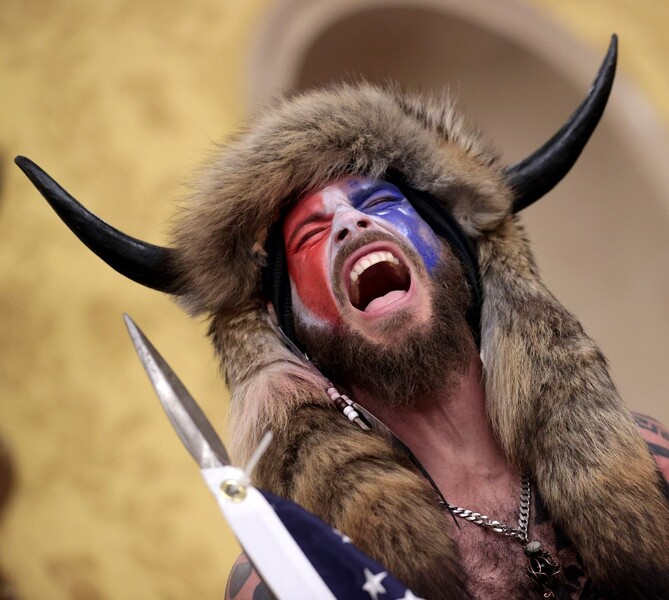
\includegraphics[max height = 0.3\textheight]{Images/qshaman.jpeg}

        \vspace*{.5em}

        (Here's some trivia: This particular devil actually lives with his mother.)
    }{}

    \vspace*{.9em}
    Please mute yourselves!
    \end{center}


    \vfill
  \end{frame}
}

\AtBeginSubsection[]{
  \begin{frame}
    \vfill
    \centering
    \begin{beamercolorbox}[sep=8pt,center,shadow=true,rounded=true]{title}
    \usebeamerfont{title}\insertsectionhead\par%
    \usebeamerfont{subtitle}\insertsubsectionhead\par%
    \end{beamercolorbox}
    \ifthenelse{\equal{\subsecname}{Answers}} {
        \begin{center}
        Unmute yourselves!
        \end{center}
    }
    \vfill
  \end{frame}
}
\begin{document}

\title{Welcome to Quarantine Trivia XV!}
\date{}

\begin{frame}
\titlepage{}
\begin{center}
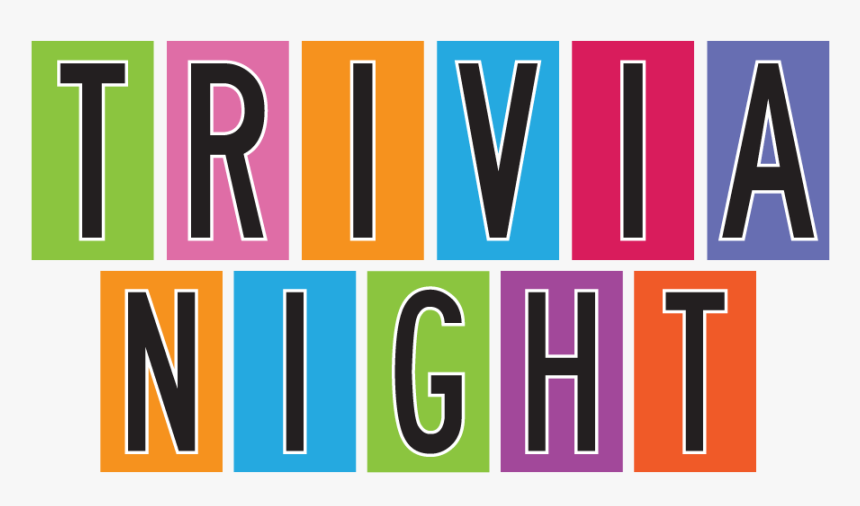
\includegraphics[max width=0.9\textwidth,
    max height=0.4\textheight]{Images/triviatitleframelogo.png}
\end{center}
\end{frame}

\begin{frame}[t]{Question 1}
\vspace{-0.5em}
\begin{block}{Question}
Which player's birthday is today?
\end{block}

\visible<2->{
    \begin{block}{Answer}
    Kathleen O'Keefe. Happy birthday, Kathleen!
    \end{block}
}
\end{frame}

\begin{frame}
This week, we couldn't resist putting a trivia spin on the prevailing meme.
\pause{}
\begin{center}
% 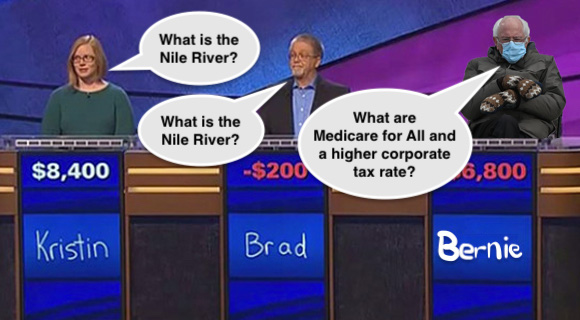
\includegraphics[max width=.95\textwidth,
% max height=0.55\textheight]{Images/bernie.jpg}
\end{center}
\end{frame}

\begin{frame}
And one last thing before we begin: By the end of this game, you will have answered
over 1,500 trivia questions.
\pause{}
\\
\bigskip
(And by our estimation, almost 100 of them were not \mbox{challenged}.)
\end{frame}

\begingroup{}
\begingroup{}
\begin{frame}[t]{Categories}
This week, you'll be answering questions in the following categories:
\begin{enumerate}
\item Black History
\item Famous Movie Lines
\item Mark Twain
\item World Currencies
\item Transportation
\item Swindlers, Frauds, and Cheats
\item Architects and Architecture
\item Paris
\item Religions and Religion
\item Museums of the World
\item Bonus Round
\end{enumerate}
\end{frame}
\endgroup{}

\begingroup{}
\begin{frame}
\vfill{}
\begin{beamercolorbox}[sep=8pt,center,shadow=true,rounded=true]{title}
\usebeamerfont{title}Good luck everyone! And have fun!
\end{beamercolorbox}
\vfill{}
\end{frame}
\endgroup{}
\def\thisSectionName{Black History}
\section{Round 1}
\subsection*{Q1}
\begin{frame}[t]{Round 1 --- Black History --- \mbox{Question 1}}
\vspace{-0.5em}
\begin{block}{Question}
Which African American is widely regarded as the first person killed in the Boston Massacre, making him the first person to die for the American Revolution?
\end{block}
\end{frame}
\subsection*{Q2}
\begin{frame}[t]{Round 1 --- Black History --- \mbox{Question 2}}
\vspace{-0.5em}
\begin{columns}[T,totalwidth=\linewidth]
\begin{column}{0.32\linewidth}
\begin{block}{Question}
Who is the girl depicted in this Normal Rockwell painting, \emph{The Problem We All Live With}, who had to be escorted to school by U.S. marshals?
\end{block}
\end{column}
\begin{column}{0.65\linewidth}
\begin{center}
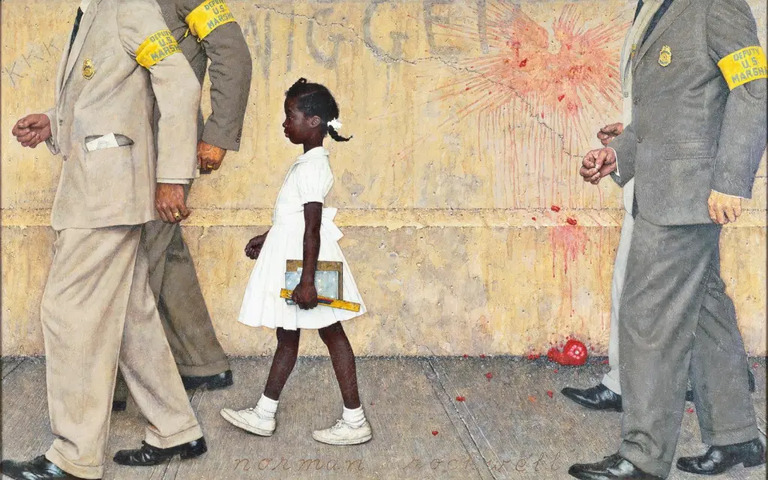
\includegraphics[max width=0.95\textwidth,max height=0.7\textheight]{{Images/rubybridges}.jpg}
\end{center}
\end{column}
\end{columns}
\end{frame}
\subsection*{Q3}
\begin{frame}[t]{Round 1 --- Black History --- \mbox{Question 3}}
\vspace{-0.5em}
\begin{block}{Question}
To within five years, in what year was the NAACP founded?
\end{block}
\end{frame}
\subsection*{Q4}
\begin{frame}[t]{Round 1 --- Black History --- \mbox{Question 4}}
\vspace{-0.5em}
\begin{block}{Question}
Which famous Black orator and abolitionist --- himself an escaped slave --- wrote an autobiography titled \emph{Narrative of the Life of [his name], an American Slave}?
\end{block}
\end{frame}
\subsection*{Q5}
\begin{frame}[t]{Round 1 --- Black History --- \mbox{Question 5}}
\vspace{-0.5em}
\begin{block}{Question}
Which African-American basketball player broke the color barrier in the NBA\@?
\end{block}
\end{frame}
\subsection*{Q6}
\begin{frame}[t]{Round 1 --- Black History --- \mbox{Question 6}}
\vspace{-0.5em}
\begin{block}{Question}
In 1957, President Eisenhower issued Executive Order 10730, which federalized which state's national guard in order to ensure the safe integration of a high school?
\end{block}
\end{frame}
\subsection*{Q7}
\begin{frame}[t]{Round 1 --- Black History --- \mbox{Question 7}}
\vspace{-0.5em}
\begin{block}{Question}
In 1921, using arms and aircraft provided by city officials, Whites attacked the people and destroyed the businesses of one of the wealthiest Black neighborhoods in the country, called ``Black Wall Street''. In which city did this disgraceful event take place?
\end{block}
\end{frame}
\subsection*{Q8}
\begin{frame}[t]{Round 1 --- Black History --- \mbox{Question 8}}
\vspace{-0.5em}
\begin{block}{Question}
Sworn into the Senate in 1870, who was the first African American to become a U.S. senator?
\end{block}
\end{frame}
\subsection*{Q9}
\begin{frame}[t]{Round 1 --- Black History --- \mbox{Question 9}}
\vspace{-0.5em}
\begin{block}{Question}
Which U.S. president first recognized Black History Month?
\end{block}
\end{frame}
\subsection*{Q10}
\begin{frame}[t]{Round 1 --- Black History --- \mbox{Question 10}}
\vspace{-0.5em}
\begin{block}{Question}
What was the name of the 20\textsuperscript{th} century African-American physician who did important research work in the area of blood transfusion and who was also among the first to promote the use of bloodmobiles?
\end{block}
\end{frame}
\subsection{Answers}
\begin{frame}[t]{Round 1 --- Black History --- \mbox{Answer 1}}
\vspace{-0.5em}
\begin{block}{Question}
Which African American is widely regarded as the first person killed in the Boston Massacre, making him the first person to die for the American Revolution?
\end{block}

\visible<2->{
    \begin{columns}[T,totalwidth=\linewidth]
    \begin{column}{0.32\linewidth}
    \begin{block}{Answer}
    Crispus Attucks
    \end{block}
    \end{column}
    \begin{column}{0.65\linewidth}
    \begin{center}
    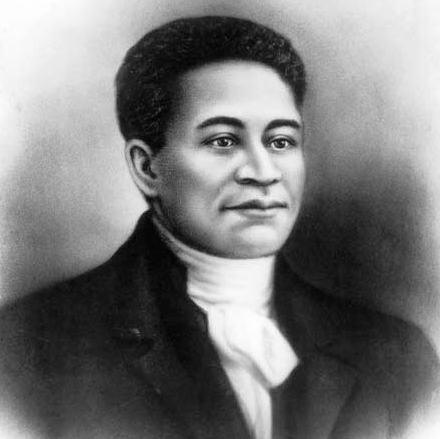
\includegraphics[max height=.45\textheight,
        max width=0.95\textwidth]{{Images/crispusattucks}.jpg}
    \end{center}
    \end{column}
    \end{columns}
}
\end{frame}
\begin{frame}[t]{Round 1 --- Black History --- \mbox{Answer 2}}
\vspace{-0.5em}
\begin{columns}[T,totalwidth=\linewidth]
\begin{column}{0.32\linewidth}
\begin{block}{Question}
Who is the girl depicted in this Normal Rockwell painting, \emph{The Problem We All Live With}, who had to be escorted to school by U.S. marshals?
\end{block}
\visible<2->{
    \begin{block}{Answer}
    Ruby Bridges
    \end{block}
}
\end{column}
\begin{column}{0.65\linewidth}
\begin{center}
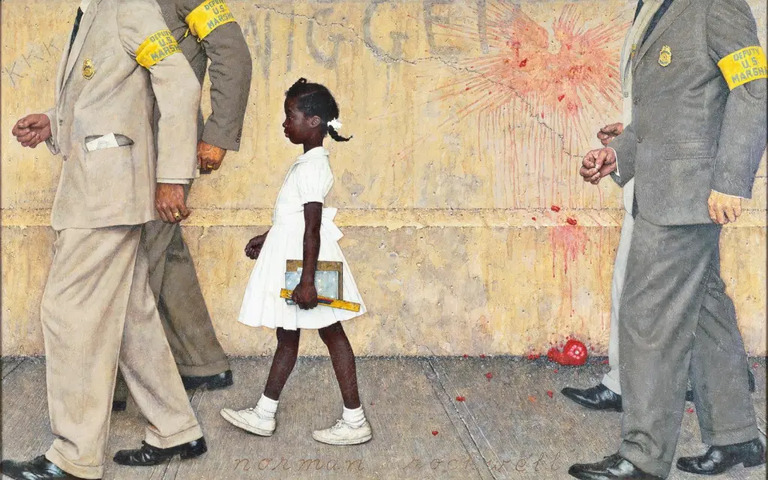
\includegraphics[max width=0.95\textwidth,max height=0.7\textheight]{{Images/rubybridges}.jpg}
\end{center}
\end{column}
\end{columns}
\end{frame}
\begin{frame}[t]{Round 1 --- Black History --- \mbox{Answer 3}}
\vspace{-0.5em}
\begin{block}{Question}
To within five years, in what year was the NAACP founded?
\end{block}

\visible<2->{
    \begin{columns}[T,totalwidth=\linewidth]
    \begin{column}{0.32\linewidth}
    \begin{block}{Answer}
    1909 (1904--1914 will be accepted)
    \end{block}
    \end{column}
    \begin{column}{0.65\linewidth}
    \begin{center}
    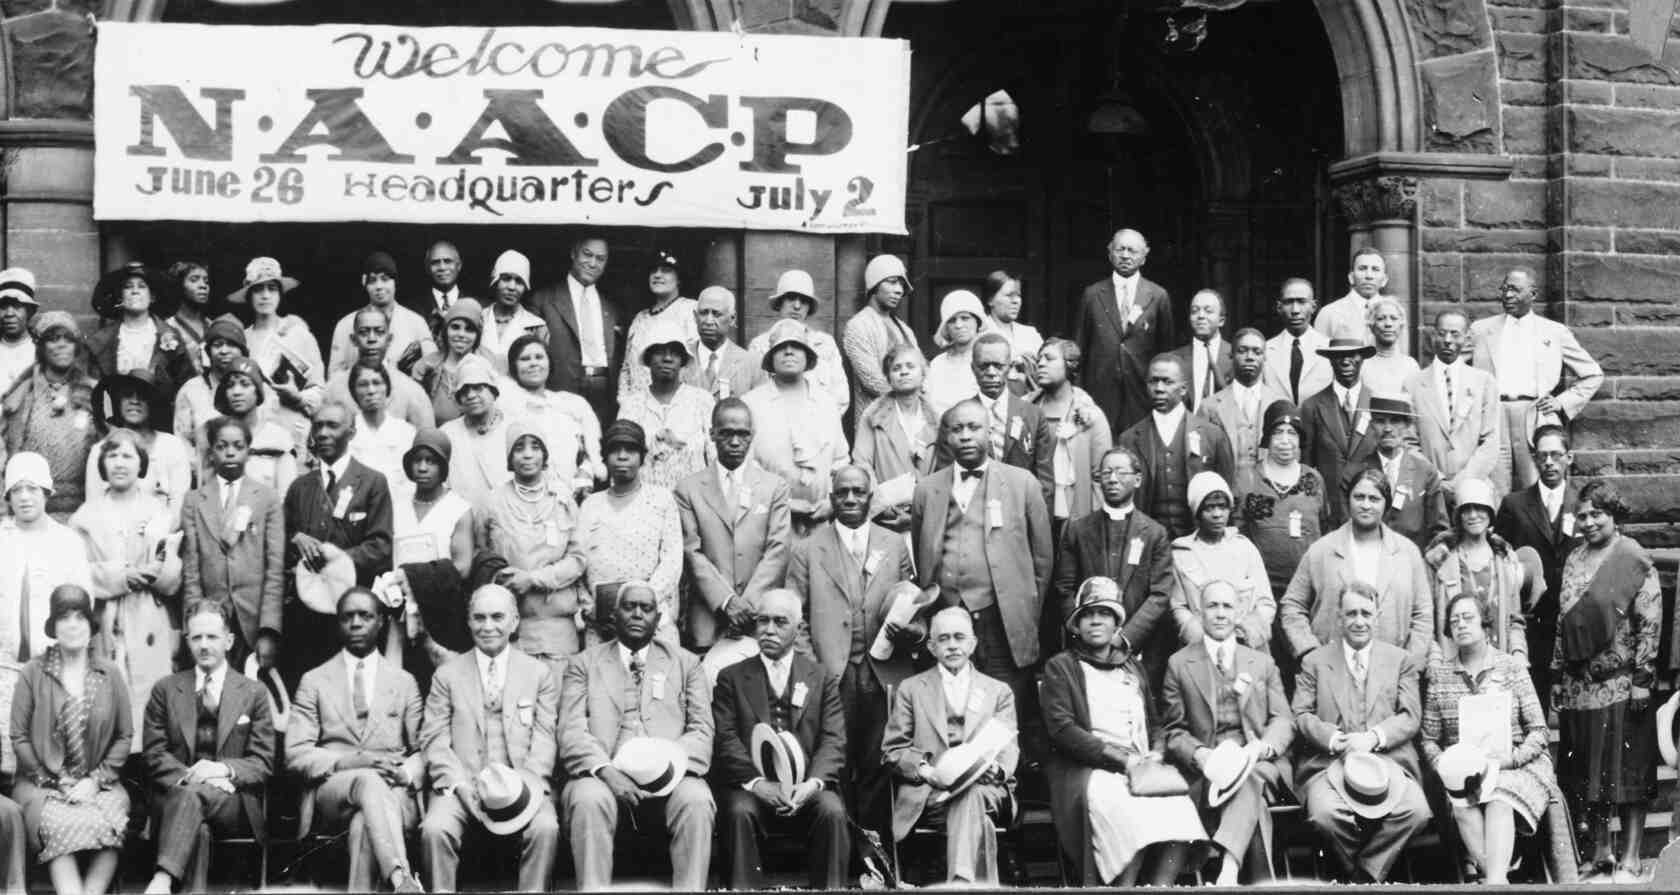
\includegraphics[max height=.45\textheight,
        max width=0.95\textwidth]{{Images/naacp}.jpg}
    \end{center}
    \end{column}
    \end{columns}
}
\end{frame}
\begin{frame}[t]{Round 1 --- Black History --- \mbox{Answer 4}}
\vspace{-0.5em}
\begin{block}{Question}
Which famous Black orator and abolitionist --- himself an escaped slave --- wrote an autobiography titled \emph{Narrative of the Life of [his name], an American Slave}?
\end{block}

\visible<2->{
    \begin{columns}[T,totalwidth=\linewidth]
    \begin{column}{0.32\linewidth}
    \begin{block}{Answer}
    Frederick Douglass
    \end{block}
    \end{column}
    \begin{column}{0.65\linewidth}
    \begin{center}
    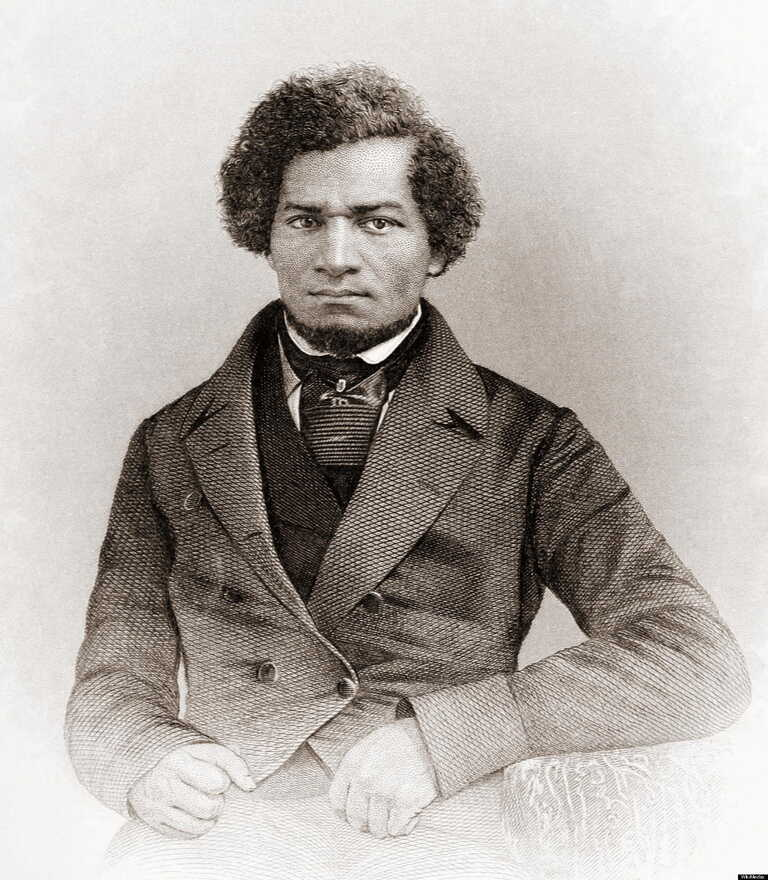
\includegraphics[max height=.45\textheight,
        max width=0.95\textwidth]{{Images/douglass}.jpg}
    \end{center}
    \end{column}
    \end{columns}
}
\end{frame}
\begin{frame}[t]{Round 1 --- Black History --- \mbox{Answer 5}}
\vspace{-0.5em}
\begin{block}{Question}
Which African-American basketball player broke the color barrier in the NBA\@?
\end{block}

\visible<2->{
    \begin{columns}[T,totalwidth=\linewidth]
    \begin{column}{0.32\linewidth}
    \begin{block}{Answer}
    Earl Lloyd
    \end{block}
    \end{column}
    \begin{column}{0.65\linewidth}
    \begin{center}
    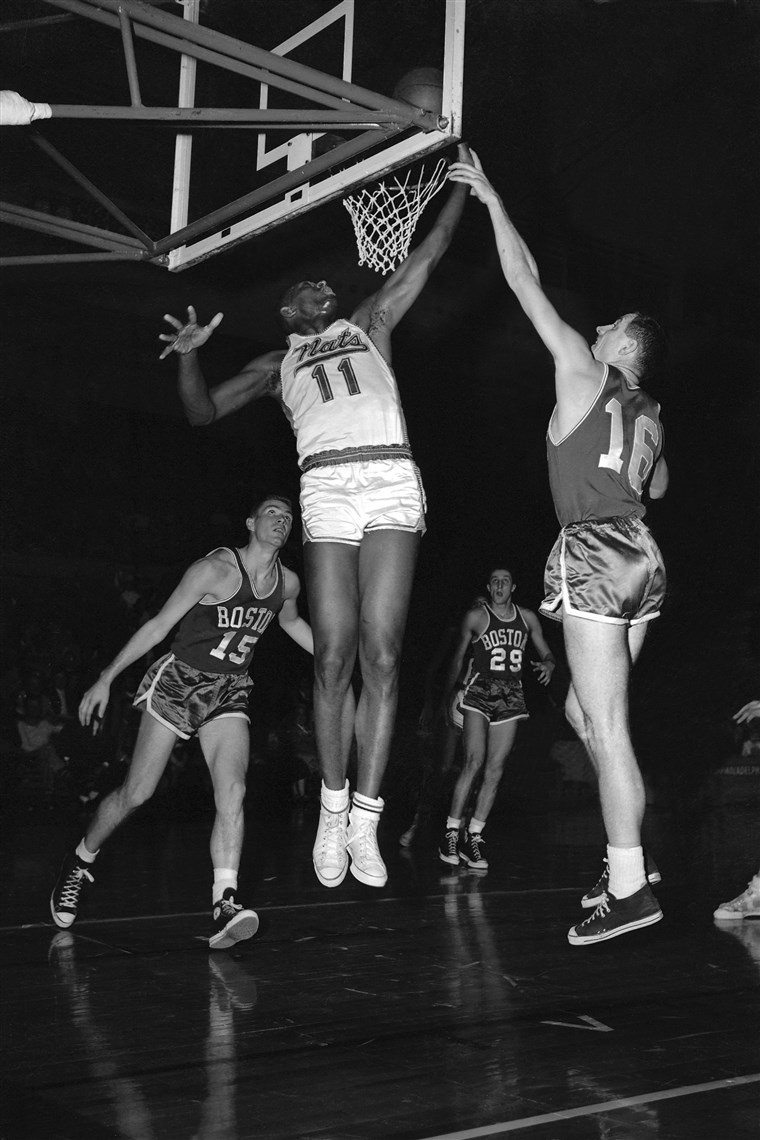
\includegraphics[max height=.45\textheight,
        max width=0.95\textwidth]{{Images/lloyd}.jpg}
    \end{center}
    \end{column}
    \end{columns}
}
\end{frame}
\begin{frame}[t]{Round 1 --- Black History --- \mbox{Answer 6}}
\vspace{-0.5em}
\begin{block}{Question}
In 1957, President Eisenhower issued Executive Order 10730, which federalized which state's national guard in order to ensure the safe integration of a high school?
\end{block}

\visible<2->{
    \begin{columns}[T,totalwidth=\linewidth]
    \begin{column}{0.32\linewidth}
    \begin{block}{Answer}
    Arkansas (in order to ensure that the Little Rock Nine could safely enter the high school in which they were enrolled)
    \end{block}
    \end{column}
    \begin{column}{0.65\linewidth}
    \begin{center}
    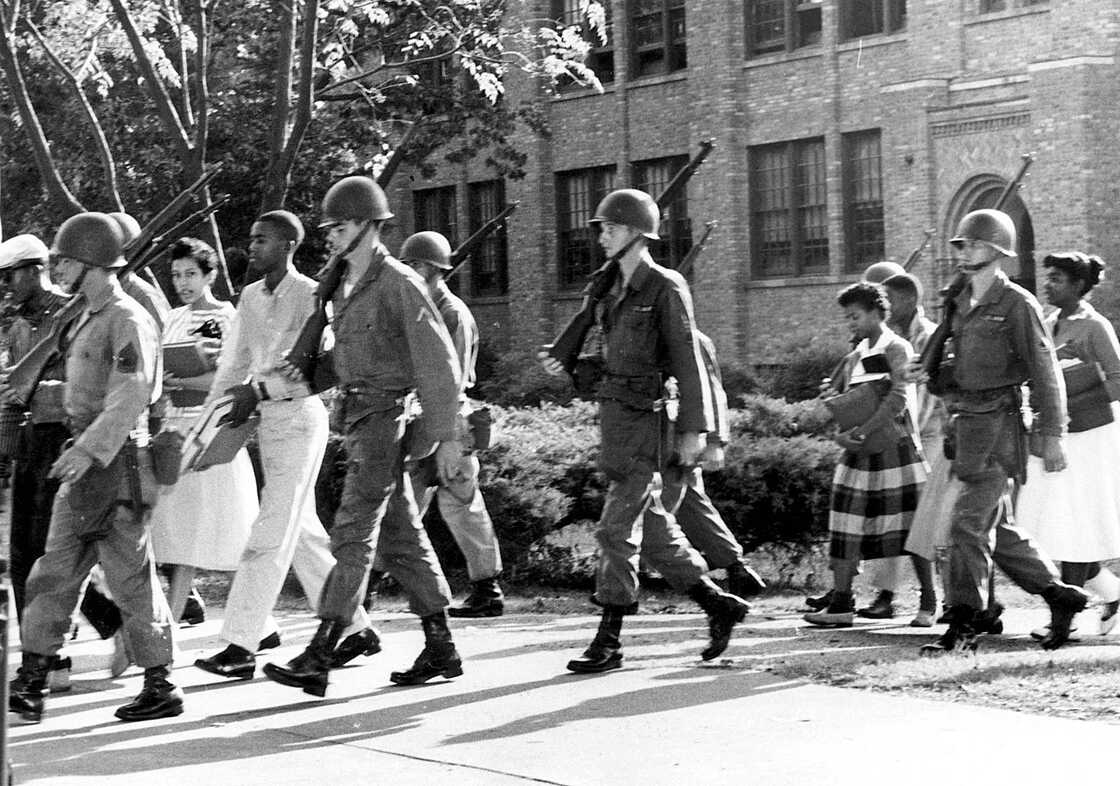
\includegraphics[max height=.45\textheight,
        max width=0.95\textwidth]{{Images/lr9}.jpg}
    \end{center}
    \end{column}
    \end{columns}
}
\end{frame}
\begin{frame}[t]{Round 1 --- Black History --- \mbox{Answer 7}}
\vspace{-0.5em}
\begin{block}{Question}
In 1921, using arms and aircraft provided by city officials, Whites attacked the people and destroyed the businesses of one of the wealthiest Black neighborhoods in the country, called ``Black Wall Street''. In which city did this disgraceful event take place?
\end{block}

\visible<2->{
    \begin{columns}[T,totalwidth=\linewidth]
    \begin{column}{0.32\linewidth}
    \begin{block}{Answer}
    Tulsa, OK
    \end{block}
    \end{column}
    \begin{column}{0.65\linewidth}
    \begin{center}
    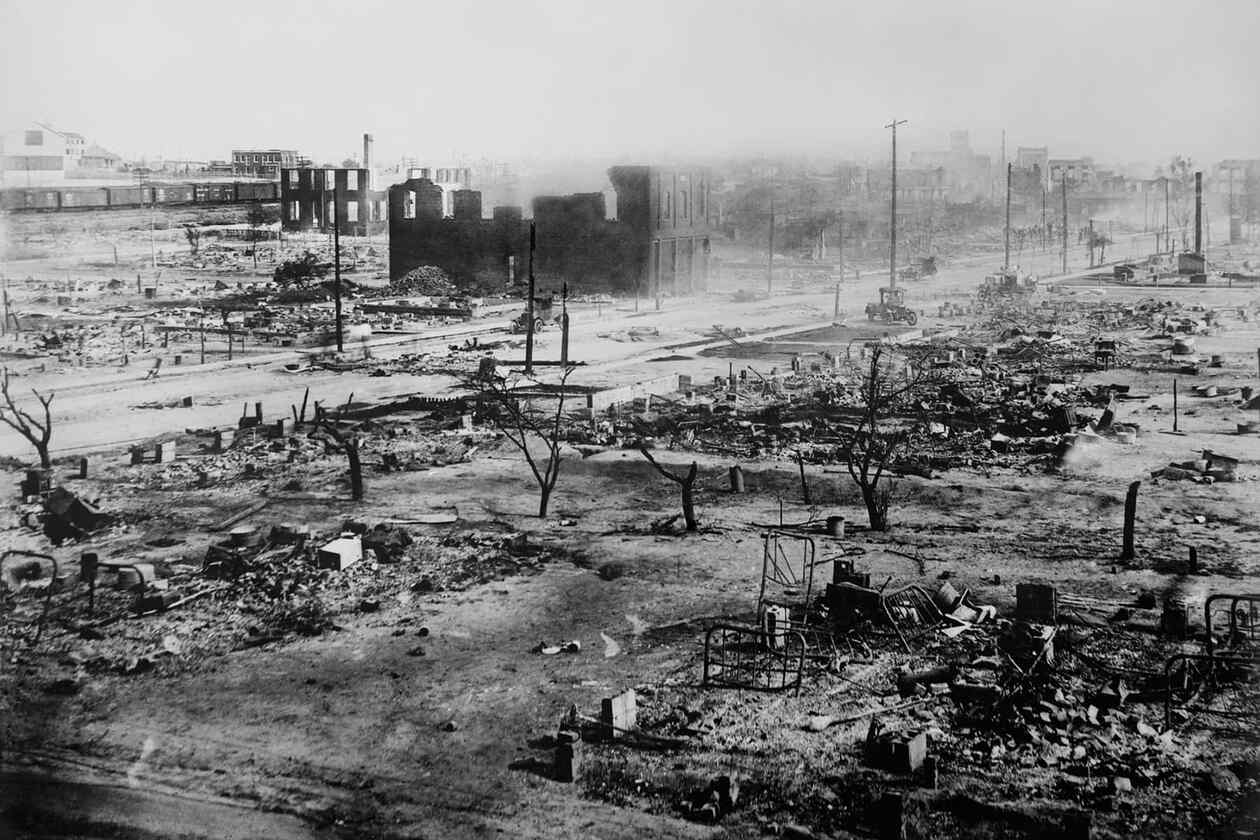
\includegraphics[max height=.45\textheight,
        max width=0.95\textwidth]{{Images/tulsa}.jpg}
    \end{center}
    \end{column}
    \end{columns}
}
\end{frame}
\begin{frame}[t]{Round 1 --- Black History --- \mbox{Answer 8}}
\vspace{-0.5em}
\begin{block}{Question}
Sworn into the Senate in 1870, who was the first African American to become a U.S. senator?
\end{block}

\visible<2->{
    \begin{columns}[T,totalwidth=\linewidth]
    \begin{column}{0.32\linewidth}
    \begin{block}{Answer}
    Hiram Revels
    \end{block}
    \end{column}
    \begin{column}{0.65\linewidth}
    \begin{center}
    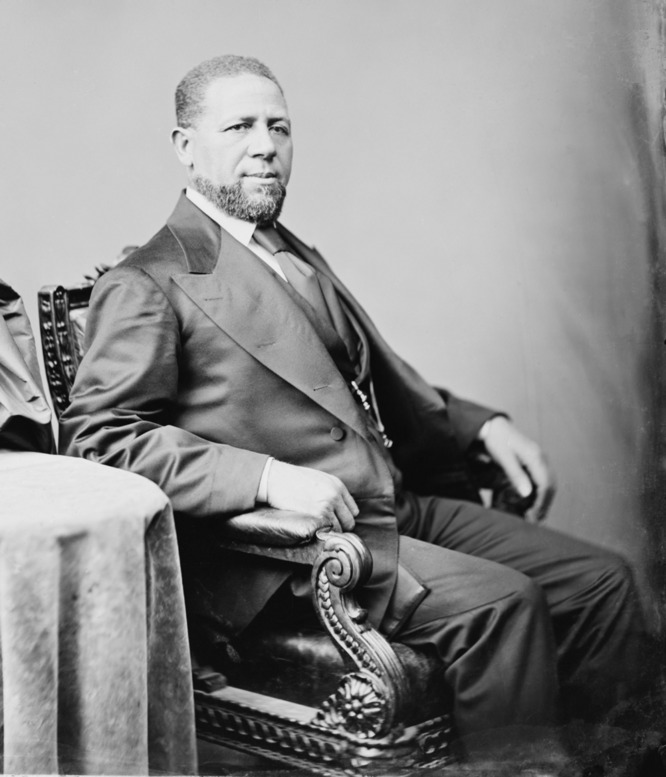
\includegraphics[max height=.45\textheight,
        max width=0.95\textwidth]{{Images/hiram}.jpg}
    \end{center}
    \end{column}
    \end{columns}
}
\end{frame}
\begin{frame}[t]{Round 1 --- Black History --- \mbox{Answer 9}}
\vspace{-0.5em}
\begin{block}{Question}
Which U.S. president first recognized Black History Month?
\end{block}

\visible<2->{
    \begin{columns}[T,totalwidth=\linewidth]
    \begin{column}{0.32\linewidth}
    \begin{block}{Answer}
    Gerald Ford (in 1976)
    \end{block}
    \end{column}
    \begin{column}{0.65\linewidth}
    \begin{center}
    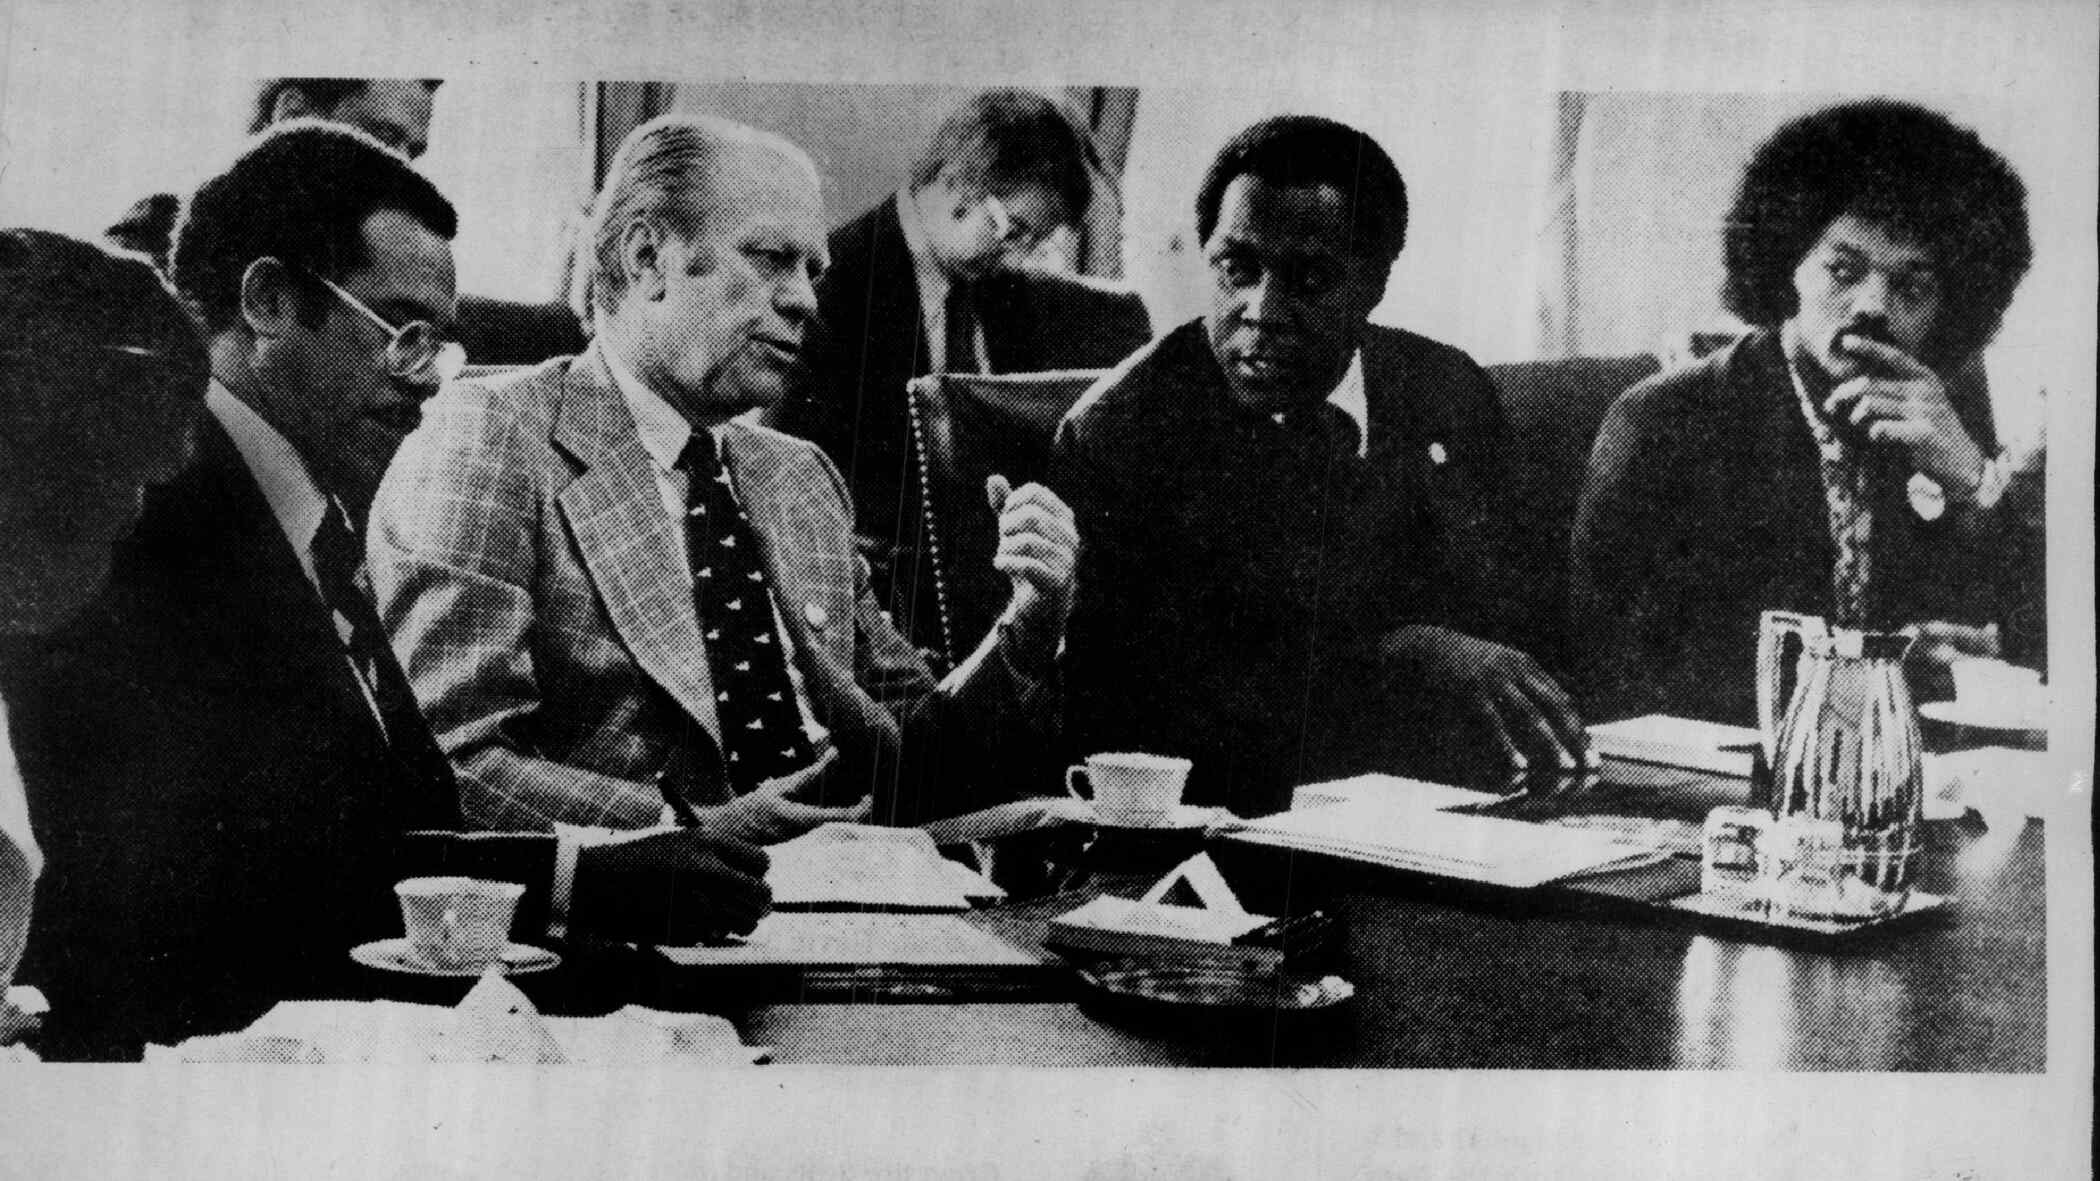
\includegraphics[max height=.45\textheight,
        max width=0.95\textwidth]{{Images/ford}.jpg}
    \end{center}
    \end{column}
    \end{columns}
}
\end{frame}
\begin{frame}[t]{Round 1 --- Black History --- \mbox{Answer 10}}
\vspace{-0.5em}
\begin{block}{Question}
What was the name of the 20\textsuperscript{th} century African-American physician who did important research work in the area of blood transfusion and who was also among the first to promote the use of bloodmobiles?
\end{block}

\visible<2->{
    \begin{columns}[T,totalwidth=\linewidth]
    \begin{column}{0.32\linewidth}
    \begin{block}{Answer}
    Dr.\ Charles Richard Drew
    \end{block}
    \end{column}
    \begin{column}{0.65\linewidth}
    \begin{center}
    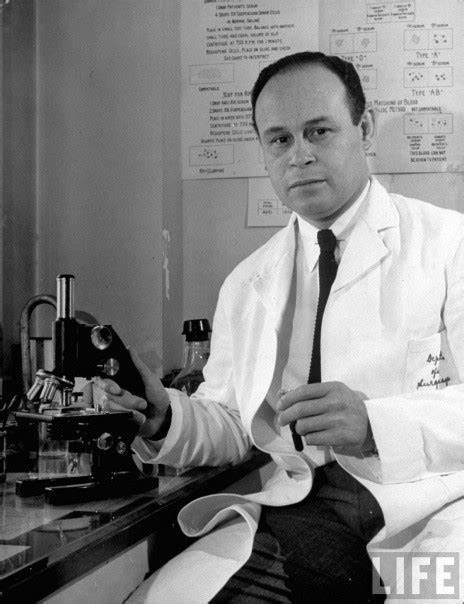
\includegraphics[max height=.45\textheight,
        max width=0.95\textwidth]{{Images/drew}.jpeg}
    \end{center}
    \end{column}
    \end{columns}
}
\end{frame}
\def\thisSectionName{Famous Movie Lines}
\section{Round 2}
\subsection*{Q1}
\begin{frame}[t]{Round 2 --- Famous Movie Lines --- \mbox{Question 1}}
\vspace{-0.5em}
\begin{block}{Question}
Which character sang the words ``\Acht{} Just keep swimming \AAcht{} Just keep swimming \Acht{}''?
\end{block}
\end{frame}
\subsection*{Q2}
\begin{frame}[t]{Round 2 --- Famous Movie Lines --- \mbox{Question 2}}
\vspace{-0.5em}
\begin{block}{Question}
In which Marx Brothers film does Groucho say, ``One morning I shot an elephant in my pajamas. How he got in my pajamas, I don't know''?
\end{block}
\end{frame}
\subsection*{Q3}
\begin{frame}[t]{Round 2 --- Famous Movie Lines --- \mbox{Question 3}}
\vspace{-0.5em}
\begin{block}{Question}
Which movie is this quote from:\par\begin{quote}And [the Dalai Lama] says, ``Oh, uh, there won't be any money, but when you die, on your deathbed, you will receive total consciousness.'' So I got that goin' for me, which is nice.\end{quote}
\end{block}
\end{frame}
\subsection*{Q4}
\begin{frame}[t]{Round 2 --- Famous Movie Lines --- \mbox{Question 4}}
\vspace{-0.5em}
\begin{block}{Question}
In which film does Clint Eastwood say the famous line, ``Go ahead, make my day.''?
\end{block}
\end{frame}
\subsection*{Q5}
\begin{frame}[t]{Round 2 --- Famous Movie Lines --- \mbox{Question 5}}
\vspace{-0.5em}
\begin{columns}[T,totalwidth=\linewidth]
\begin{column}{0.52\linewidth}
\begin{block}{Question}
What is actress Gloria Swanson about to utter at the moment of \emph{Sunset Boulevard} (1950) pictured here? (We're looking for a single sentence containing the phrases ``all right'' and ``close-up''. Punctuation won't matter.)
\end{block}
\end{column}
\begin{column}{0.45\linewidth}
\begin{center}
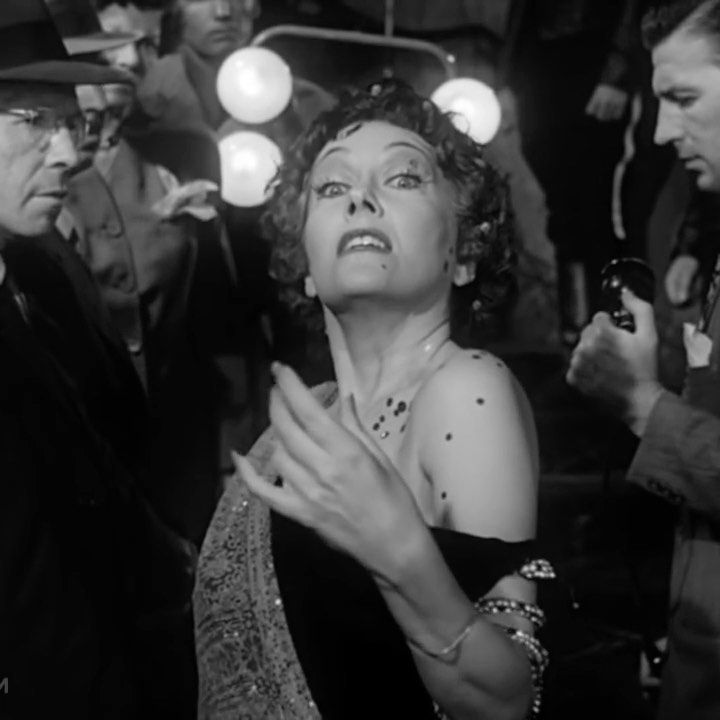
\includegraphics[max width=0.95\textwidth,max height=0.7\textheight]{{Images/demille}.jpg}
\end{center}
\end{column}
\end{columns}
\end{frame}
\subsection*{Q6}
\begin{frame}[t]{Round 2 --- Famous Movie Lines --- \mbox{Question 6}}
\vspace{-0.5em}
\begin{block}{Question}
Finish this quote from \emph{Dr.\ Strangelove} (1964): ``Gentlemen, you can't fight in here! This is the \textunderscore{}\textunderscore{}\textunderscore{}\textunderscore{}\textunderscore{} \textunderscore{}\textunderscore{}\textunderscore{}\textunderscore{}\textunderscore{}!'' (two words).
\end{block}
\end{frame}
\subsection*{Q7}
\begin{frame}[t]{Round 2 --- Famous Movie Lines --- \mbox{Question 7}}
\vspace{-0.5em}
\begin{block}{Question}
What sentence precedes Leslie Nielsen's famous line in \emph{Airplane} (1980), ``I am serious. And don't call me Shirley.''?
\end{block}
\end{frame}
\subsection*{Q8}
\begin{frame}[t]{Round 2 --- Famous Movie Lines --- \mbox{Question 8}}
\vspace{-0.5em}
\begin{block}{Question}
Which movie is this line from: ``Just one word \ldots{} Are you listening? \ldots{} Plastics.''?
\end{block}
\end{frame}
\subsection*{Q9}
\begin{frame}[t]{Round 2 --- Famous Movie Lines --- \mbox{Question 9}}
\vspace{-0.5em}
\begin{block}{Question}
Name the movie: ``Toga! Toga! Toga!''
\end{block}
\end{frame}
\subsection*{Q10}
\begin{frame}[t]{Round 2 --- Famous Movie Lines --- \mbox{Question 10}}
\vspace{-0.5em}
\begin{block}{Question}
There is one James Bond film in which Bond actually drinks his martini ``stirred, not shaken''. Which Bond film is it?
\end{block}
\end{frame}
\subsection{Answers}
\begin{frame}[t]{Round 2 --- Famous Movie Lines --- \mbox{Answer 1}}
\vspace{-0.5em}
\begin{block}{Question}
Which character sang the words ``\Acht{} Just keep swimming \AAcht{} Just keep swimming \Acht{}''?
\end{block}

\visible<2->{
    \begin{columns}[T,totalwidth=\linewidth]
    \begin{column}{0.32\linewidth}
    \begin{block}{Answer}
    Dory (in \emph{Finding nemo} (2003))
    \end{block}
    \end{column}
    \begin{column}{0.65\linewidth}
    \begin{center}
    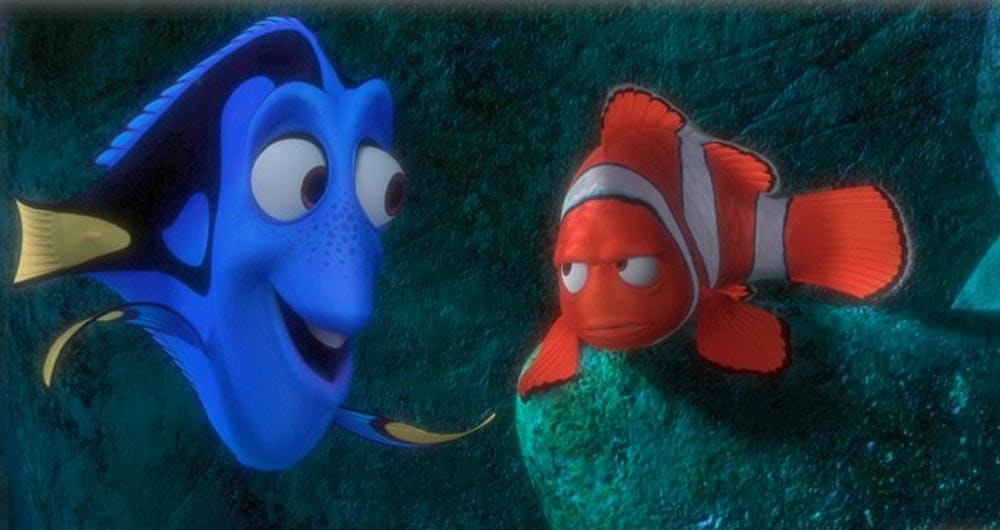
\includegraphics[max height=.45\textheight,
        max width=0.95\textwidth]{{Images/dory}.jpg}
    \end{center}
    \end{column}
    \end{columns}
}
\end{frame}
\begin{frame}[t]{Round 2 --- Famous Movie Lines --- \mbox{Answer 2}}
\vspace{-0.5em}
\begin{block}{Question}
In which Marx Brothers film does Groucho say, ``One morning I shot an elephant in my pajamas. How he got in my pajamas, I don't know''?
\end{block}

\visible<2->{
    \begin{columns}[T,totalwidth=\linewidth]
    \begin{column}{0.32\linewidth}
    \begin{block}{Answer}
    \emph{Animal Crackers} (1930)
    \end{block}
    \end{column}
    \begin{column}{0.65\linewidth}
    \begin{center}
    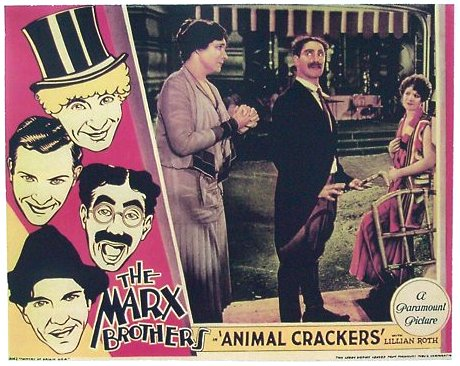
\includegraphics[max height=.45\textheight,
        max width=0.95\textwidth]{{Images/marx}.jpeg}
    \end{center}
    \end{column}
    \end{columns}
}
\end{frame}
\begin{frame}[t]{Round 2 --- Famous Movie Lines --- \mbox{Answer 3}}
\vspace{-0.5em}
\begin{block}{Question}
Which movie is this quote from:\par\begin{quote}And [the Dalai Lama] says, ``Oh, uh, there won't be any money, but when you die, on your deathbed, you will receive total consciousness.'' So I got that goin' for me, which is nice.\end{quote}
\end{block}

\visible<2->{
    \begin{columns}[T,totalwidth=\linewidth]
    \begin{column}{0.32\linewidth}
    \begin{block}{Answer}
    \emph{Caddyshack} (1980)
    \end{block}
    \end{column}
    \begin{column}{0.65\linewidth}
    \begin{center}
    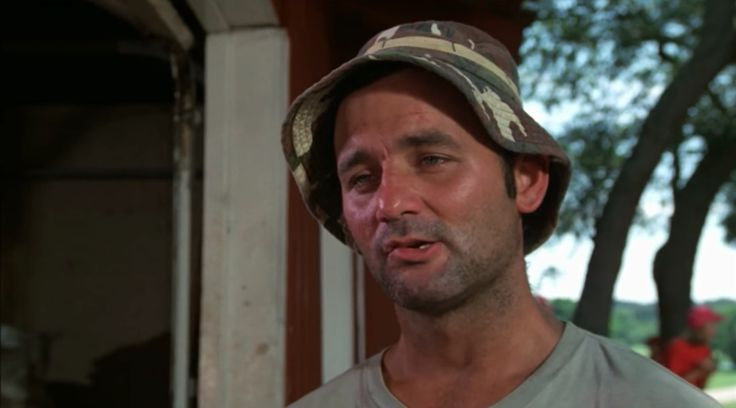
\includegraphics[max height=.45\textheight,
        max width=0.95\textwidth]{{Images/caddyshack}.jpeg}
    \end{center}
    \end{column}
    \end{columns}
}
\end{frame}
\begin{frame}[t]{Round 2 --- Famous Movie Lines --- \mbox{Answer 4}}
\vspace{-0.5em}
\begin{block}{Question}
In which film does Clint Eastwood say the famous line, ``Go ahead, make my day.''?
\end{block}

\visible<2->{
    \begin{columns}[T,totalwidth=\linewidth]
    \begin{column}{0.32\linewidth}
    \begin{block}{Answer}
    \emph{Sudden Impact} (1983)
    \end{block}
    \end{column}
    \begin{column}{0.65\linewidth}
    \begin{center}
    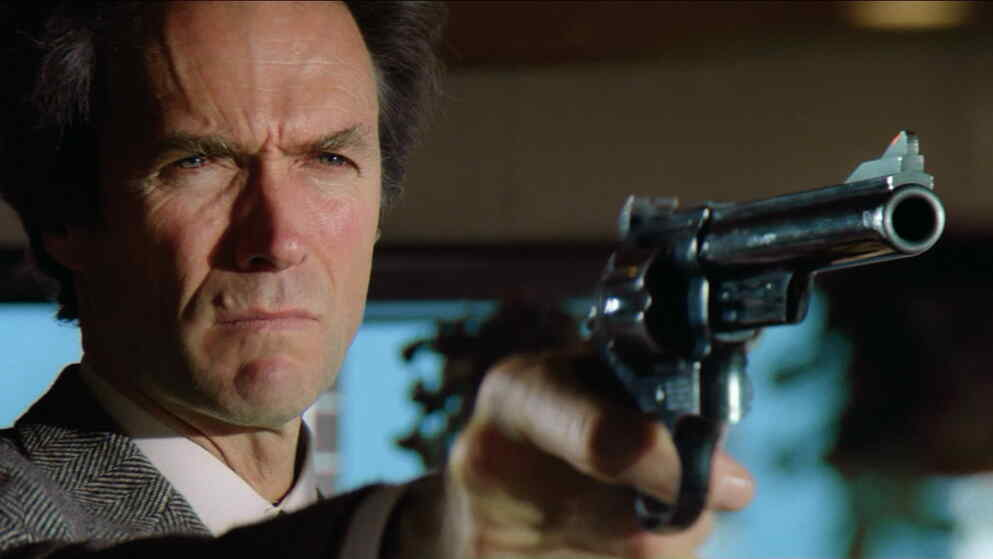
\includegraphics[max height=.45\textheight,
        max width=0.95\textwidth]{{Images/makemyday}.jpg}
    \end{center}
    \end{column}
    \end{columns}
}
\end{frame}
\begin{frame}[t]{Round 2 --- Famous Movie Lines --- \mbox{Answer 5}}
\vspace{-0.5em}
\begin{columns}[T,totalwidth=\linewidth]
\begin{column}{0.48\linewidth}
\begin{block}{Question}
What is actress Gloria Swanson about to utter at the moment of \emph{Sunset Boulevard} (1950) pictured here? (We're looking for a single sentence containing the phrases ``all right'' and ``close-up''. Punctuation won't matter.)
\end{block}
\visible<2->{
    \begin{block}{Answer}
    ``All right, Mr.\ DeMille, I'm ready for my close-up.''
    \end{block}
}
\end{column}
\begin{column}{0.5\linewidth}
\begin{center}
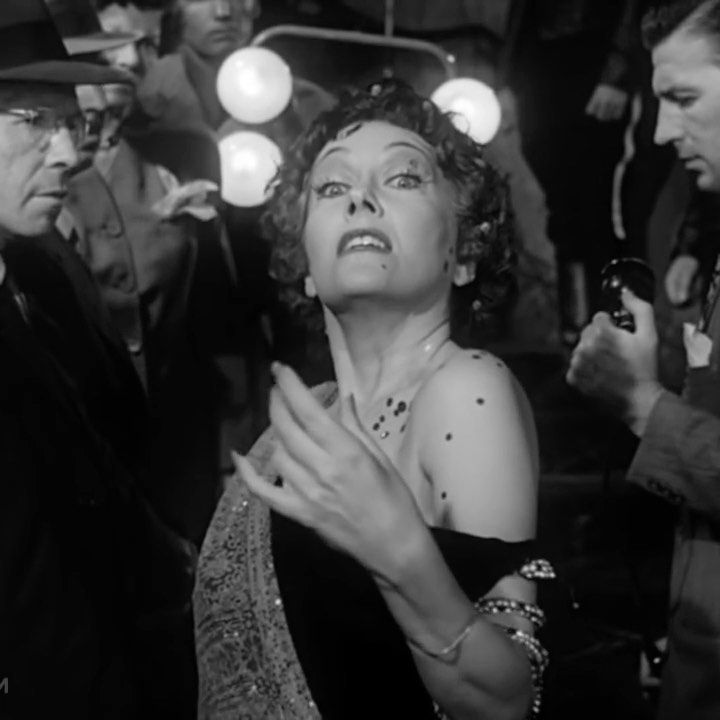
\includegraphics[max width=0.95\textwidth,max height=0.7\textheight]{{Images/demille}.jpg}
\end{center}
\end{column}
\end{columns}
\end{frame}
\begin{frame}[t]{Round 2 --- Famous Movie Lines --- \mbox{Answer 6}}
\vspace{-0.5em}
\begin{block}{Question}
Finish this quote from \emph{Dr.\ Strangelove} (1964): ``Gentlemen, you can't fight in here! This is the \textunderscore{}\textunderscore{}\textunderscore{}\textunderscore{}\textunderscore{} \textunderscore{}\textunderscore{}\textunderscore{}\textunderscore{}\textunderscore{}!'' (two words).
\end{block}

\visible<2->{
    \begin{columns}[T,totalwidth=\linewidth]
    \begin{column}{0.32\linewidth}
    \begin{block}{Answer}
    War Room
    \end{block}
    \end{column}
    \begin{column}{0.65\linewidth}
    \begin{center}
    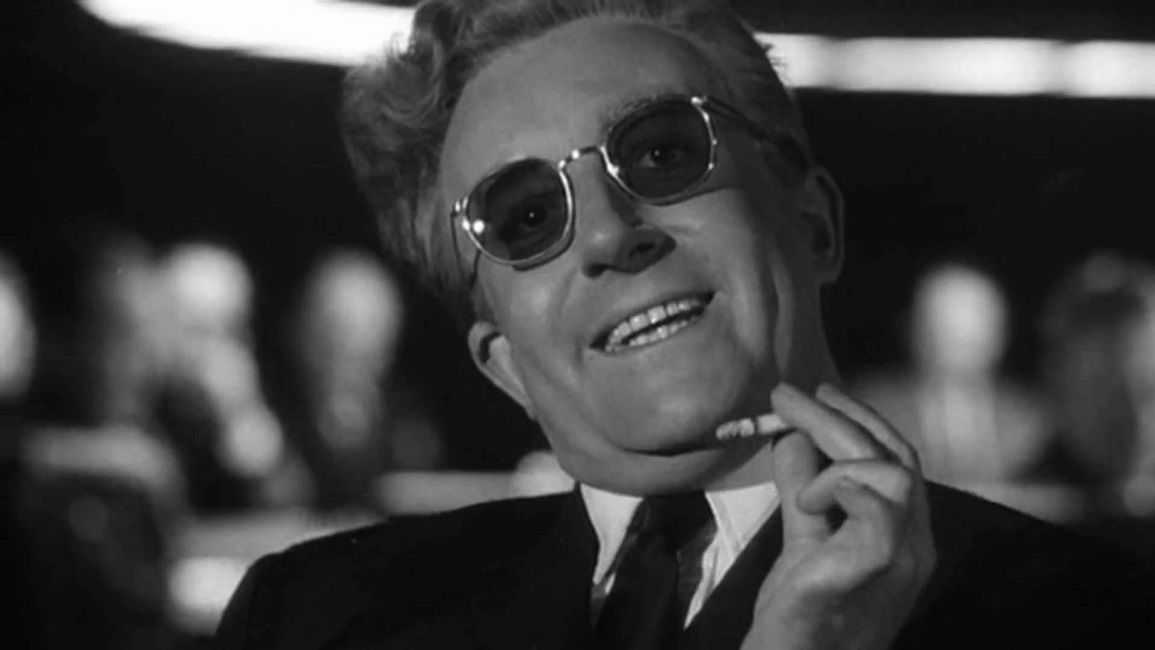
\includegraphics[max height=.45\textheight,
        max width=0.95\textwidth]{{Images/strangelove}.jpg}
    \end{center}
    \end{column}
    \end{columns}
}
\end{frame}
\begin{frame}[t]{Round 2 --- Famous Movie Lines --- \mbox{Answer 7}}
\vspace{-0.5em}
\begin{block}{Question}
What sentence precedes Leslie Nielsen's famous line in \emph{Airplane} (1980), ``I am serious. And don't call me Shirley.''?
\end{block}

\visible<2->{
    \begin{columns}[T,totalwidth=\linewidth]
    \begin{column}{0.32\linewidth}
    \begin{block}{Answer}
    ``Surely you can't be serious \textinterrobang{}''
    \end{block}
    \end{column}
    \begin{column}{0.65\linewidth}
    \begin{center}
    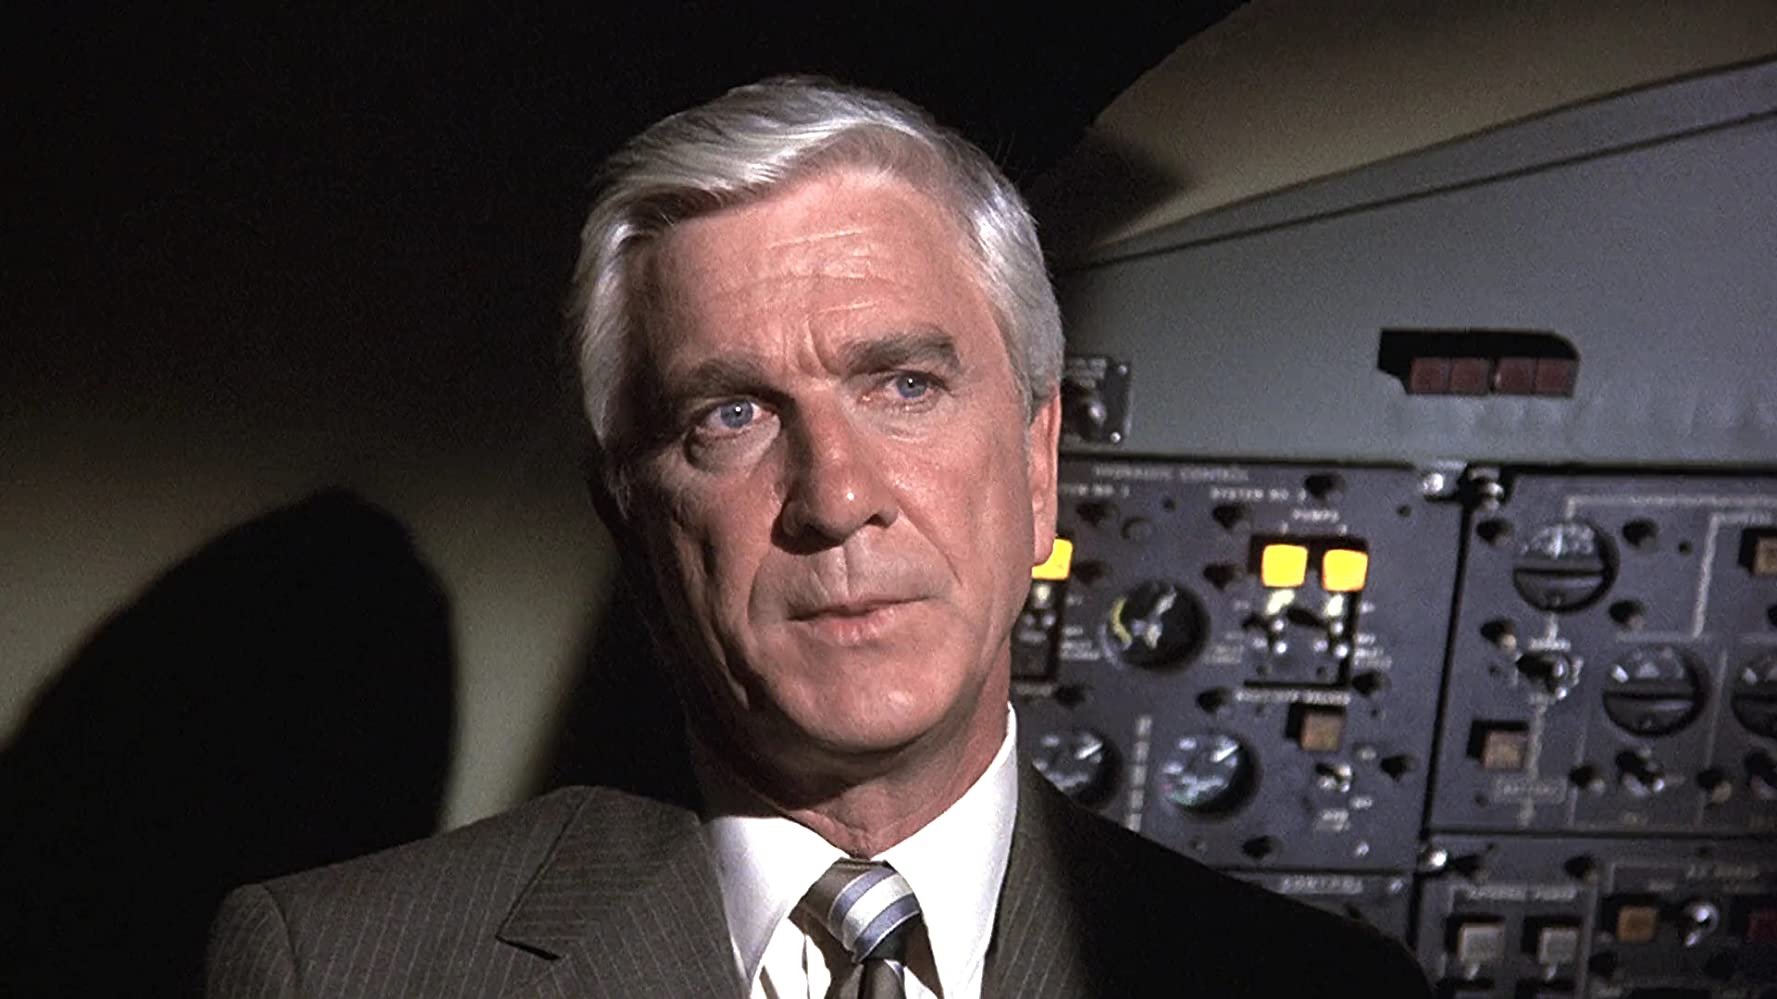
\includegraphics[max height=.45\textheight,
        max width=0.95\textwidth]{{Images/nielsen}.jpg}
    \end{center}
    \end{column}
    \end{columns}
}
\end{frame}
\begin{frame}[t]{Round 2 --- Famous Movie Lines --- \mbox{Answer 8}}
\vspace{-0.5em}
\begin{block}{Question}
Which movie is this line from: ``Just one word \ldots{} Are you listening? \ldots{} Plastics.''?
\end{block}

\visible<2->{
    \begin{columns}[T,totalwidth=\linewidth]
    \begin{column}{0.32\linewidth}
    \begin{block}{Answer}
    \emph{The Graduate} (1967)
    \end{block}
    \end{column}
    \begin{column}{0.65\linewidth}
    \begin{center}
    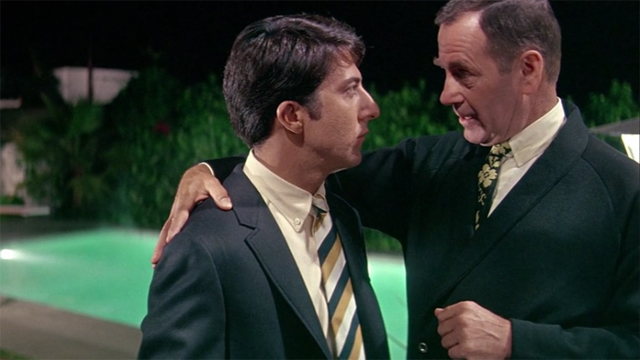
\includegraphics[max height=.45\textheight,
        max width=0.95\textwidth]{{Images/plastics}.jpg}
    \end{center}
    \end{column}
    \end{columns}
}
\end{frame}
\begin{frame}[t]{Round 2 --- Famous Movie Lines --- \mbox{Answer 9}}
\vspace{-0.5em}
\begin{block}{Question}
Name the movie: ``Toga! Toga! Toga!''
\end{block}

\visible<2->{
    \begin{columns}[T,totalwidth=\linewidth]
    \begin{column}{0.32\linewidth}
    \begin{block}{Answer}
    \emph{Animal House} (1978)
    \end{block}
    \end{column}
    \begin{column}{0.65\linewidth}
    \begin{center}
    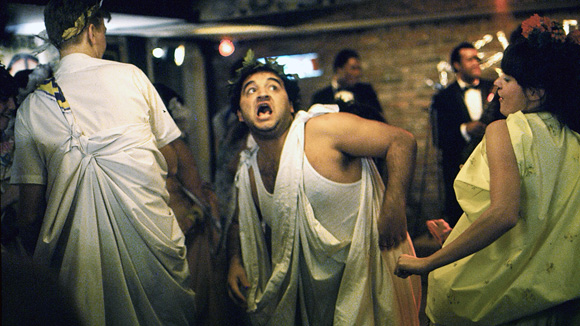
\includegraphics[max height=.45\textheight,
        max width=0.95\textwidth]{{Images/toga}.jpeg}
    \end{center}
    \end{column}
    \end{columns}
}
\end{frame}
\begin{frame}[t]{Round 2 --- Famous Movie Lines --- \mbox{Answer 10}}
\vspace{-0.5em}
\begin{block}{Question}
There is one James Bond film in which Bond actually drinks his martini ``stirred, not shaken''. Which Bond film is it?
\end{block}

\visible<2->{
    \begin{columns}[T,totalwidth=\linewidth]
    \begin{column}{0.32\linewidth}
    \begin{block}{Answer}
    \emph{You Only Live Twice} (1967)
    \end{block}
    \end{column}
    \begin{column}{0.65\linewidth}
    \begin{center}
    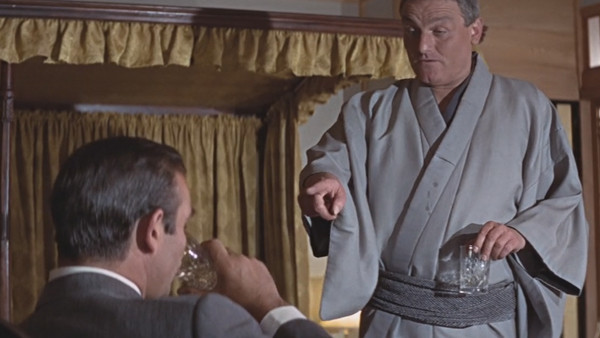
\includegraphics[max height=.45\textheight,
        max width=0.95\textwidth]{{Images/bond}.jpg}
    \end{center}
    \end{column}
    \end{columns}
}
\end{frame}
\def\thisSectionName{Mark Twain}
\section{Round 3}
\subsection*{Q1}
\begin{frame}[t]{Round 3 --- Mark Twain --- \mbox{Question 1}}
\vspace{-0.5em}
\begin{block}{Question}
In what state was Mark Twain born?
\end{block}
\end{frame}
\subsection*{Q2}
\begin{frame}[t]{Round 3 --- Mark Twain --- \mbox{Question 2}}
\vspace{-0.5em}
\begin{block}{Question}
What was Mark Twain's birth name? (We need his middle name too. Spelling won't count.)
\end{block}
\end{frame}
\subsection*{Q3}
\begin{frame}[t]{Round 3 --- Mark Twain --- \mbox{Question 3}}
\vspace{-0.5em}
\begin{block}{Question}
What Mark Twain novel featured a time-traveler?
\end{block}
\end{frame}
\subsection*{Q4}
\begin{frame}[t]{Round 3 --- Mark Twain --- \mbox{Question 4}}
\vspace{-0.5em}
\begin{block}{Question}
In later life, what color suit did Mark Twain famously wear?
\end{block}
\end{frame}
\subsection*{Q5}
\begin{frame}[t]{Round 3 --- Mark Twain --- \mbox{Question 5}}
\vspace{-0.5em}
\begin{block}{Question}
On December 17, 1877, Twain attended a Boston dinner in honor of the poet John Greenleaf Whittier. In attendance, among other notables, were Emerson, Holmes and Longfellow.  Twain did something that night that he regretted for the rest of his life. What did he do? 
\end{block}
\end{frame}
\subsection*{Q6}
\begin{frame}[t]{Round 3 --- Mark Twain --- \mbox{Question 6}}
\vspace{-0.5em}
\begin{block}{Question}
What was Mark Twain's best selling novel during his lifetime?
\end{block}
\end{frame}
\subsection*{Q7}
\begin{frame}[t]{Round 3 --- Mark Twain --- \mbox{Question 7}}
\vspace{-0.5em}
\begin{block}{Question}
Before he became a literary figure, Twain had another occupation in which he wrote a lot.  What was it?
\end{block}
\end{frame}
\subsection*{Q8}
\begin{frame}[t]{Round 3 --- Mark Twain --- \mbox{Question 8}}
\vspace{-0.5em}
\begin{block}{Question}
What deeply biting and sarcastic collection of Twain essays was not published until 1939, long after Twain's death?
\end{block}
\end{frame}
\subsection*{Q9}
\begin{frame}[t]{Round 3 --- Mark Twain --- \mbox{Question 9}}
\vspace{-0.5em}
\begin{block}{Question}
Within five years either way, when was Twain born and when did he die?
\end{block}
\end{frame}
\subsection*{Q10}
\begin{frame}[t]{Round 3 --- Mark Twain --- \mbox{Question 10}}
\vspace{-0.5em}
\begin{block}{Question}
Twain had a friendship with another famous figure who said of Twain, ``He treated me like a competent human being, That's why I loved him.'' Twain said of this friend, ``I am filled with the wonder of [my friend's] knowledge, acquired because shut out from all distractions.''
\end{block}
\end{frame}
\subsection{Answers}
\begin{frame}[t]{Round 3 --- Mark Twain --- \mbox{Answer 1}}
\vspace{-0.5em}
\begin{block}{Question}
In what state was Mark Twain born?
\end{block}

\visible<2->{
    \begin{columns}[T,totalwidth=\linewidth]
    \begin{column}{0.32\linewidth}
    \begin{block}{Answer}
    Missouri 
    \end{block}
    \end{column}
    \begin{column}{0.65\linewidth}
    \begin{center}
    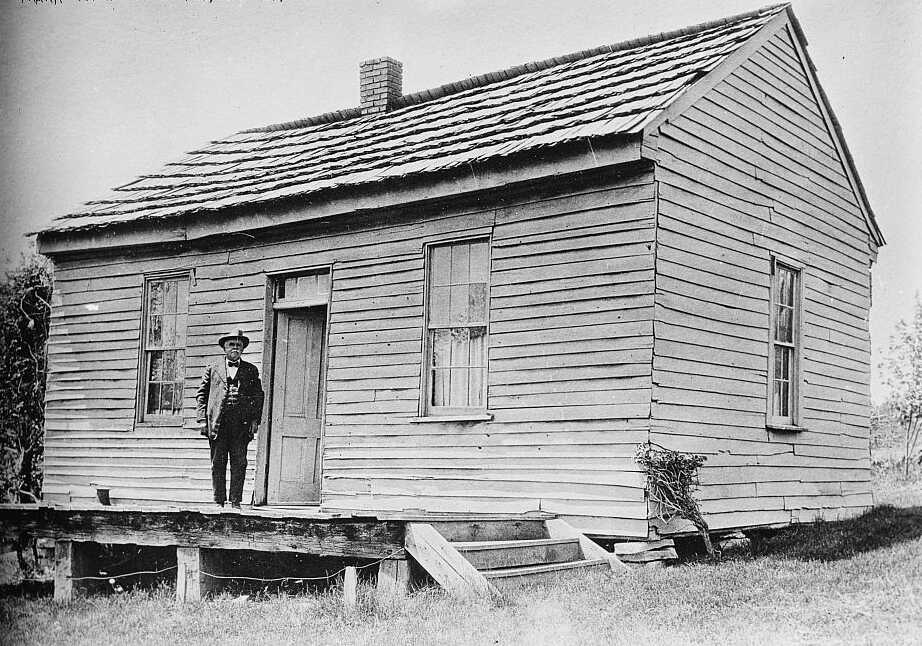
\includegraphics[max height=.45\textheight,
        max width=0.95\textwidth]{{Images/floridamo}.jpg}
    \end{center}
    \end{column}
    \end{columns}
}
\end{frame}
\begin{frame}[t]{Round 3 --- Mark Twain --- \mbox{Answer 2}}
\vspace{-0.5em}
\begin{block}{Question}
What was Mark Twain's birth name? (We need his middle name too. Spelling won't count.)
\end{block}
\visible<2->{
    \begin{block}{Answer}
    Samuel Langhorne Clemens
    \end{block}
}
\end{frame}
\begin{frame}[t]{Round 3 --- Mark Twain --- \mbox{Answer 3}}
\vspace{-0.5em}
\begin{block}{Question}
What Mark Twain novel featured a time-traveler?
\end{block}

\visible<2->{
    \begin{columns}[T,totalwidth=\linewidth]
    \begin{column}{0.32\linewidth}
    \begin{block}{Answer}
    A Connecticut Yankee in King Arthur's Court 
    \end{block}
    \end{column}
    \begin{column}{0.65\linewidth}
    \begin{center}
    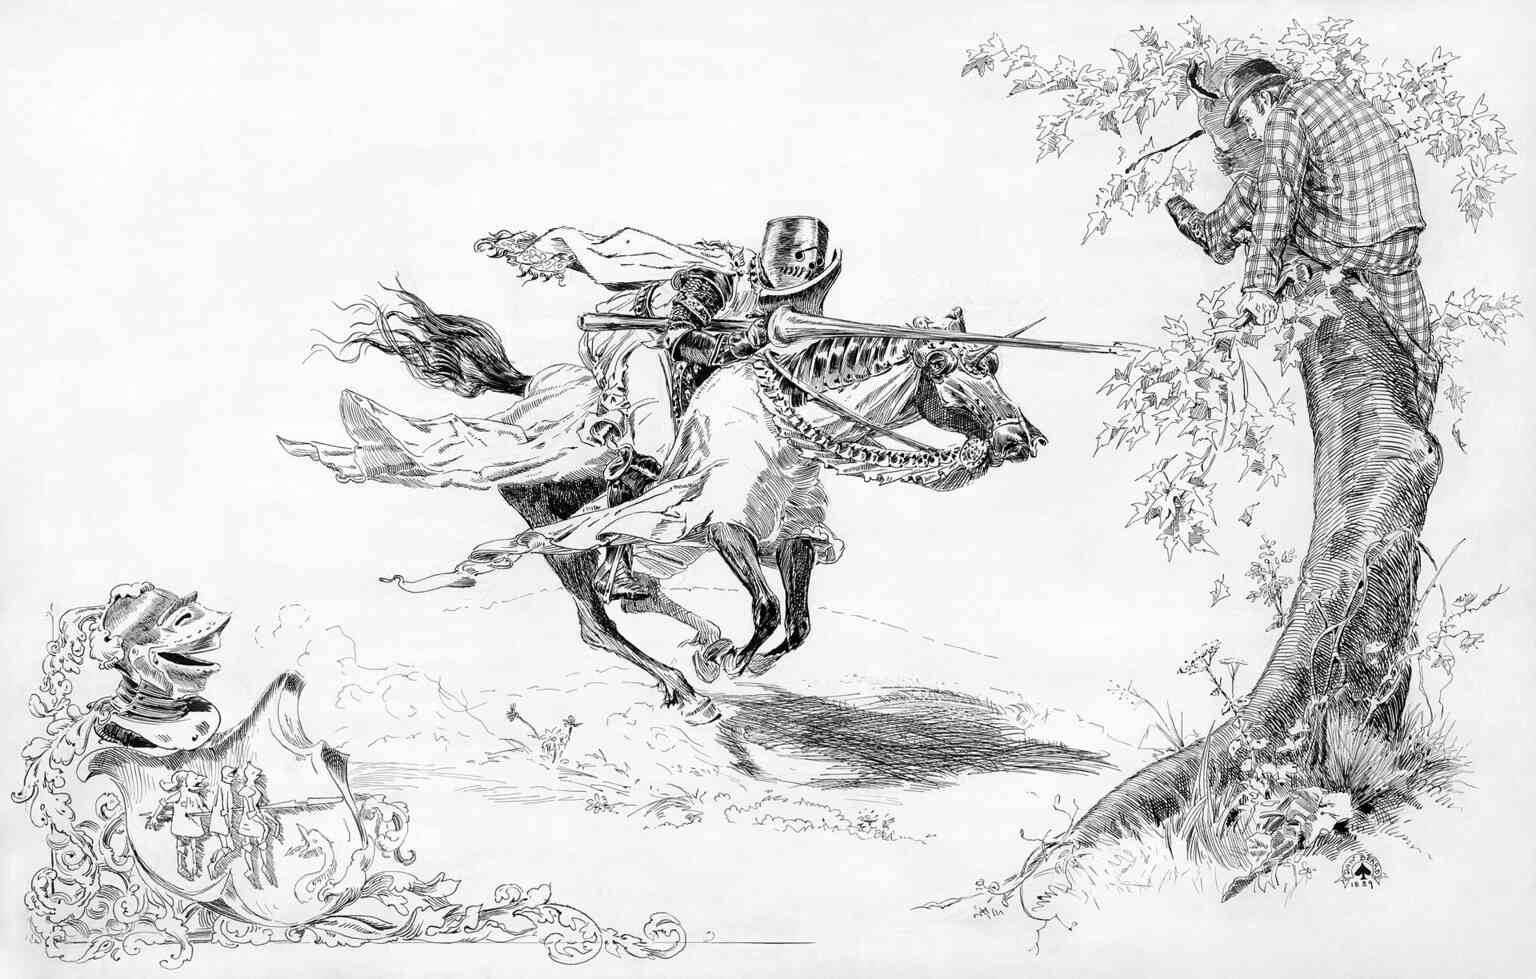
\includegraphics[max height=.45\textheight,
        max width=0.95\textwidth]{{Images/connyank}.jpg}
    \end{center}
    \end{column}
    \end{columns}
}
\end{frame}
\begin{frame}[t]{Round 3 --- Mark Twain --- \mbox{Answer 4}}
\vspace{-0.5em}
\begin{block}{Question}
In later life, what color suit did Mark Twain famously wear?
\end{block}

\visible<2->{
    \begin{columns}[T,totalwidth=\linewidth]
    \begin{column}{0.32\linewidth}
    \begin{block}{Answer}
    White
    \end{block}
    \end{column}
    \begin{column}{0.65\linewidth}
    \begin{center}
    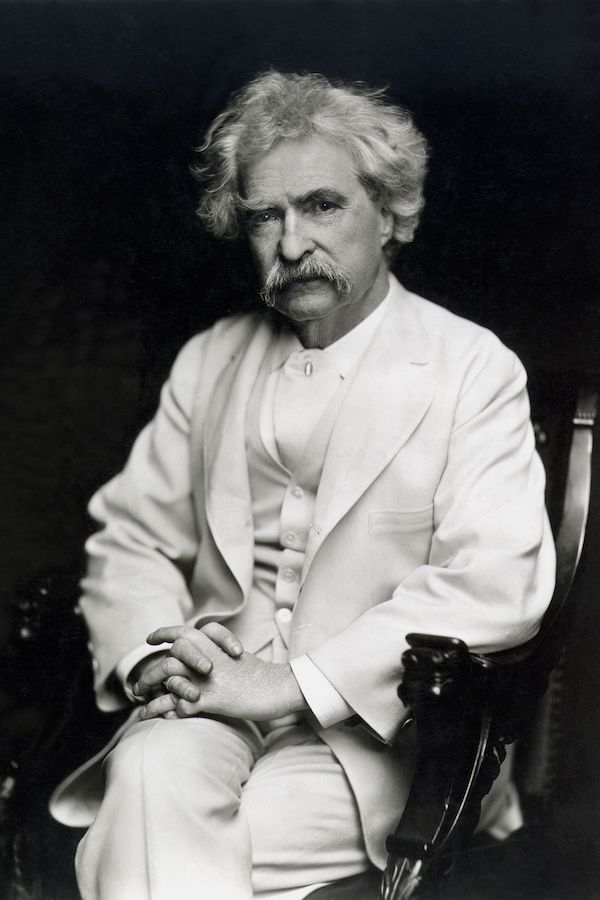
\includegraphics[max height=.45\textheight,
        max width=0.95\textwidth]{{Images/twainwhite}.jpg}
    \end{center}
    \end{column}
    \end{columns}
}
\end{frame}
\begin{frame}[t]{Round 3 --- Mark Twain --- \mbox{Answer 5}}
\vspace{-0.5em}
\begin{block}{Question}
On December 17, 1877, Twain attended a Boston dinner in honor of the poet John Greenleaf Whittier. In attendance, among other notables, were Emerson, Holmes and Longfellow.  Twain did something that night that he regretted for the rest of his life. What did he do? 
\end{block}

\visible<2->{
    \begin{columns}[T,totalwidth=\linewidth]
    \begin{column}{0.32\linewidth}
    \begin{block}{Answer}
    He made a speech in which he ``roasted'' Emerson, Holmes and Longfellow. The speech was universally criticized and Twain felt compelled to write an abject apology to the three men. 
    \end{block}
    \end{column}
    \begin{column}{0.65\linewidth}
    \begin{center}
    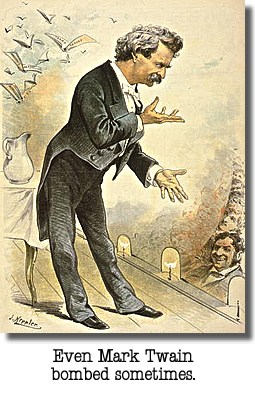
\includegraphics[max height=.45\textheight,
        max width=0.95\textwidth]{{Images/twainroast}.jpg}
    \end{center}
    \end{column}
    \end{columns}
}
\end{frame}
\begin{frame}[t]{Round 3 --- Mark Twain --- \mbox{Answer 6}}
\vspace{-0.5em}
\begin{block}{Question}
What was Mark Twain's best selling novel during his lifetime?
\end{block}

\visible<2->{
    \begin{columns}[T,totalwidth=\linewidth]
    \begin{column}{0.32\linewidth}
    \begin{block}{Answer}
    \emph{The Innocents Abroad} / \emph{The New Pilgrims' Progress}
    \end{block}
    \end{column}
    \begin{column}{0.65\linewidth}
    \begin{center}
    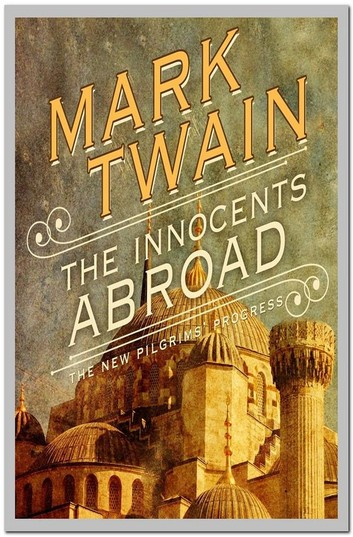
\includegraphics[max height=.45\textheight,
        max width=0.95\textwidth]{{Images/innocentsabroad}.jpg}
    \end{center}
    \end{column}
    \end{columns}
}
\end{frame}
\begin{frame}[t]{Round 3 --- Mark Twain --- \mbox{Answer 7}}
\vspace{-0.5em}
\begin{block}{Question}
Before he became a literary figure, Twain had another occupation in which he wrote a lot.  What was it?
\end{block}

\visible<2->{
    \begin{columns}[T,totalwidth=\linewidth]
    \begin{column}{0.32\linewidth}
    \begin{block}{Answer}
    Reporter
    \end{block}
    \end{column}
    \begin{column}{0.65\linewidth}
    \begin{center}
    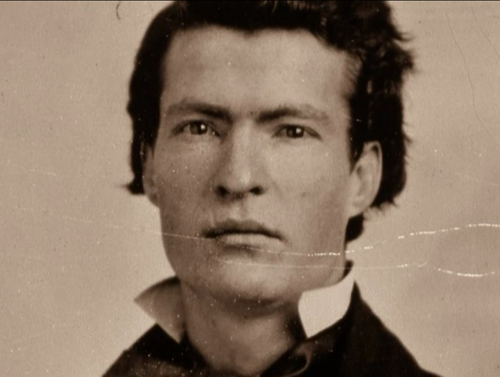
\includegraphics[max height=.45\textheight,
        max width=0.95\textwidth]{{Images/twainyoung}.png}
    \end{center}
    \end{column}
    \end{columns}
}
\end{frame}
\begin{frame}[t]{Round 3 --- Mark Twain --- \mbox{Answer 8}}
\vspace{-0.5em}
\begin{block}{Question}
What deeply biting and sarcastic collection of Twain essays was not published until 1939, long after Twain's death?
\end{block}

\visible<2->{
    \begin{columns}[T,totalwidth=\linewidth]
    \begin{column}{0.32\linewidth}
    \begin{block}{Answer}
    Letters from the Earth
    \end{block}
    \end{column}
    \begin{column}{0.65\linewidth}
    \begin{center}
    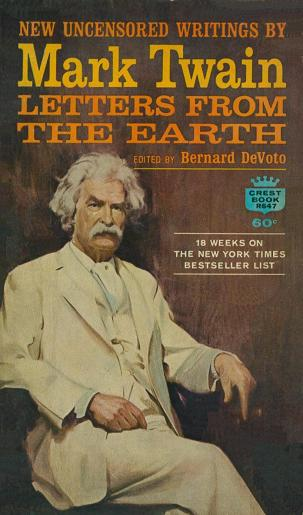
\includegraphics[max height=.45\textheight,
        max width=0.95\textwidth]{{Images/twainletters}.jpeg}
    \end{center}
    \end{column}
    \end{columns}
}
\end{frame}
\begin{frame}[t]{Round 3 --- Mark Twain --- \mbox{Answer 9}}
\vspace{-0.5em}
\begin{block}{Question}
Within five years either way, when was Twain born and when did he die?
\end{block}

\visible<2->{
    \begin{columns}[T,totalwidth=\linewidth]
    \begin{column}{0.32\linewidth}
    \begin{block}{Answer}
    Born 1835 (we'll accept 1830--1940); died 1910 (we'll accept 1905--1915).
    \end{block}
    \end{column}
    \begin{column}{0.65\linewidth}
    \begin{center}
    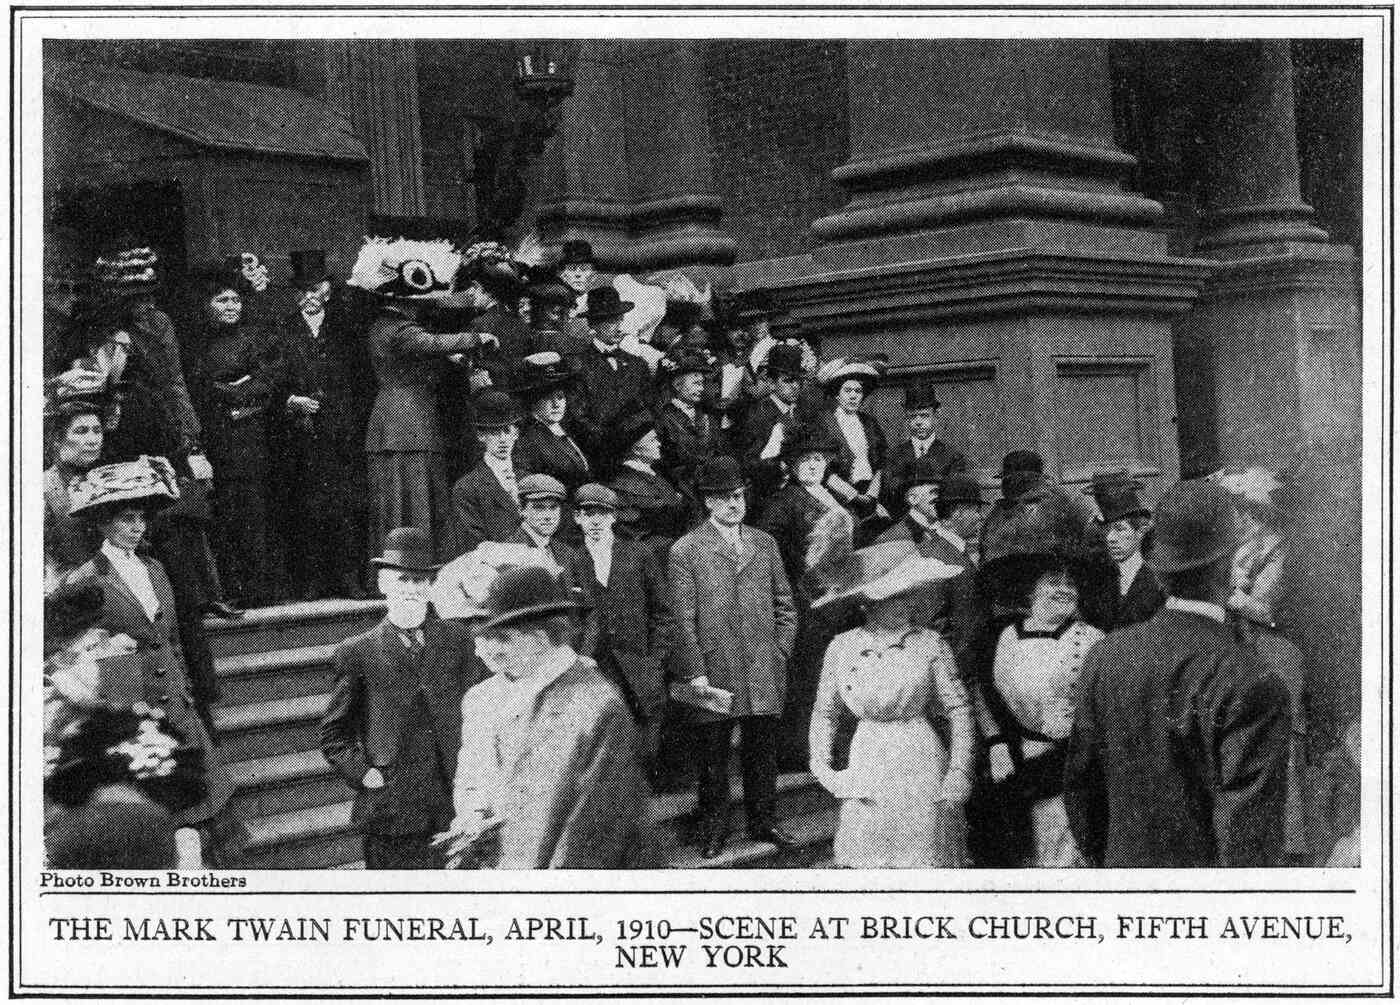
\includegraphics[max height=.45\textheight,
        max width=0.95\textwidth]{{Images/twainfuneral}.jpg}
    \end{center}
    \end{column}
    \end{columns}
}
\end{frame}
\begin{frame}[t]{Round 3 --- Mark Twain --- \mbox{Answer 10}}
\vspace{-0.5em}
\begin{block}{Question}
Twain had a friendship with another famous figure who said of Twain, ``He treated me like a competent human being, That's why I loved him.'' Twain said of this friend, ``I am filled with the wonder of [my friend's] knowledge, acquired because shut out from all distractions.''
\end{block}

\visible<2->{
    \begin{columns}[T,totalwidth=\linewidth]
    \begin{column}{0.32\linewidth}
    \begin{block}{Answer}
    Helen Keller
    \end{block}
    \end{column}
    \begin{column}{0.65\linewidth}
    \begin{center}
    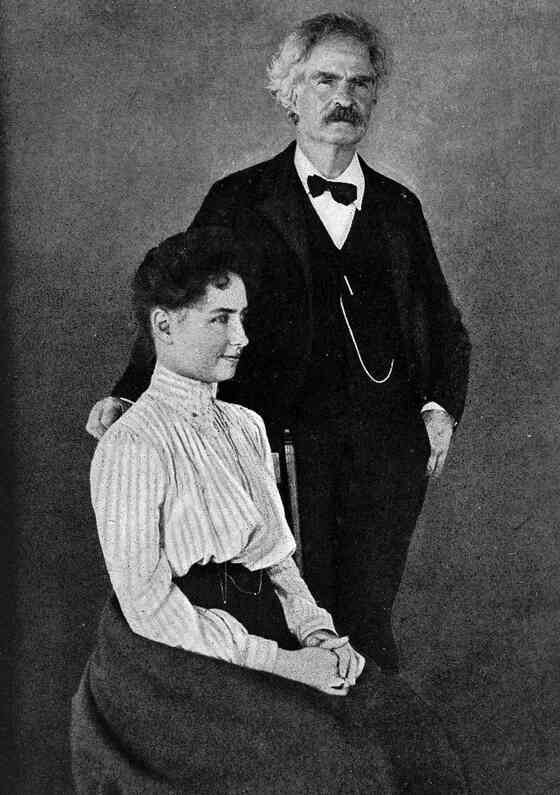
\includegraphics[max height=.45\textheight,
        max width=0.95\textwidth]{{Images/keller}.jpg}
    \end{center}
    \end{column}
    \end{columns}
}
\end{frame}
\def\thisSectionName{World Currencies}
\section{Round 4}
\subsection*{Q1}
\begin{frame}[t]{Round 4 --- World Currencies --- \mbox{Question 1}}
\vspace{-0.5em}
\begin{block}{Question}
Who is currently slated to replace Andrew Jackson on the U.S. \$20 bill?
\end{block}
\end{frame}
\subsection*{Q2}
\begin{frame}[t]{Round 4 --- World Currencies --- \mbox{Question 2}}
\vspace{-0.5em}
\begin{block}{Question}
One one-hundredth of which currency is called a \emph{Rappen} in German, a \emph{centime} in French, a \emph{centesimo} in Italian, and a \emph{rap} in Romansch?
\end{block}
\end{frame}
\subsection*{Q3}
\begin{frame}[t]{Round 4 --- World Currencies --- \mbox{Question 3}}
\vspace{-0.5em}
\begin{block}{Question}
Which country calls their currency's one- and two-dollar coins the ``Loonie'' and the ``Toonie'', respectively?
\end{block}
\end{frame}
\subsection*{Q4}
\begin{frame}[t]{Round 4 --- World Currencies --- \mbox{Question 4}}
\vspace{-0.5em}
\begin{block}{Question}
Which currency's three-letter code is MXN\@? (We need the country and the name of the currency.)
\end{block}
\end{frame}
\subsection*{Q5}
\begin{frame}[t]{Round 4 --- World Currencies --- \mbox{Question 5}}
\vspace{-0.5em}
\begin{block}{Question}
What is the name of the currency that became widespread in early Islamic nations and is still used in several countries, including Algeria, Iraq, and Tunisia?
\end{block}
\end{frame}
\subsection*{Q6}
\begin{frame}[t]{Round 4 --- World Currencies --- \mbox{Question 6}}
\vspace{-0.5em}
\begin{block}{Question}
What is the world's oldest currency still in use?
\end{block}
\end{frame}
\subsection*{Q7}
\begin{frame}[t]{Round 4 --- World Currencies --- \mbox{Question 7}}
\vspace{-0.5em}
\begin{block}{Question}
Which country's currency was unpegged from the U.S. dollar in 2005, prior to which it had been fixed to trade at a ratio of 8.27:\$1?
\end{block}
\end{frame}
\subsection*{Q8}
\begin{frame}[t]{Round 4 --- World Currencies --- \mbox{Question 8}}
\vspace{-0.5em}
\begin{columns}[T,totalwidth=\linewidth]
\begin{column}{0.32\linewidth}
\begin{block}{Question}
Which currency's symbol is pictured here? (We need the country and the name of the currency.)
\end{block}
\end{column}
\begin{column}{0.65\linewidth}
\begin{center}

\includegraphics[max width=0.95\textwidth,max height=0.7\textheight]{{Images/rupee}.png}
\end{center}
\end{column}
\end{columns}
\end{frame}
\subsection*{Q9}
\begin{frame}[t]{Round 4 --- World Currencies --- \mbox{Question 9}}
\vspace{-0.5em}
\begin{block}{Question}
What is the name of the smallest unit of Bitcoin, which is worth one 100-millionth of a bitcoin?
\end{block}
\end{frame}
\subsection*{Q10}
\begin{frame}[t]{Round 4 --- World Currencies --- \mbox{Question 10}}
\vspace{-0.5em}
\begin{block}{Question}
What is the official currency of both Ecuador and El Salvador?
\end{block}
\end{frame}
\subsection{Answers}
\begin{frame}[t]{Round 4 --- World Currencies --- \mbox{Answer 1}}
\vspace{-0.5em}
\begin{block}{Question}
Who is currently slated to replace Andrew Jackson on the U.S. \$20 bill?
\end{block}

\visible<2->{
    \begin{columns}[T,totalwidth=\linewidth]
    \begin{column}{0.32\linewidth}
    \begin{block}{Answer}
    Harriet Tubman
    \end{block}
    \end{column}
    \begin{column}{0.65\linewidth}
    \begin{center}
    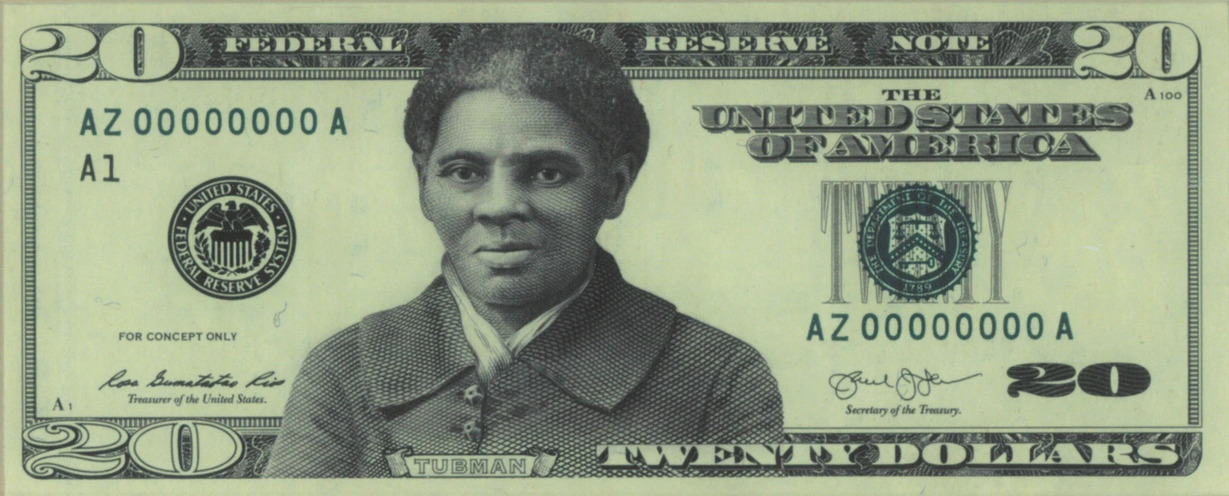
\includegraphics[max height=.45\textheight,
        max width=0.95\textwidth]{{Images/tubman}.jpg}
    \end{center}
    \end{column}
    \end{columns}
}
\end{frame}
\begin{frame}[t]{Round 4 --- World Currencies --- \mbox{Answer 2}}
\vspace{-0.5em}
\begin{block}{Question}
One one-hundredth of which currency is called a \emph{Rappen} in German, a \emph{centime} in French, a \emph{centesimo} in Italian, and a \emph{rap} in Romansch?
\end{block}

\visible<2->{
    \begin{columns}[T,totalwidth=\linewidth]
    \begin{column}{0.32\linewidth}
    \begin{block}{Answer}
    The (Swiss) franc
    \end{block}
    \end{column}
    \begin{column}{0.65\linewidth}
    \begin{center}
    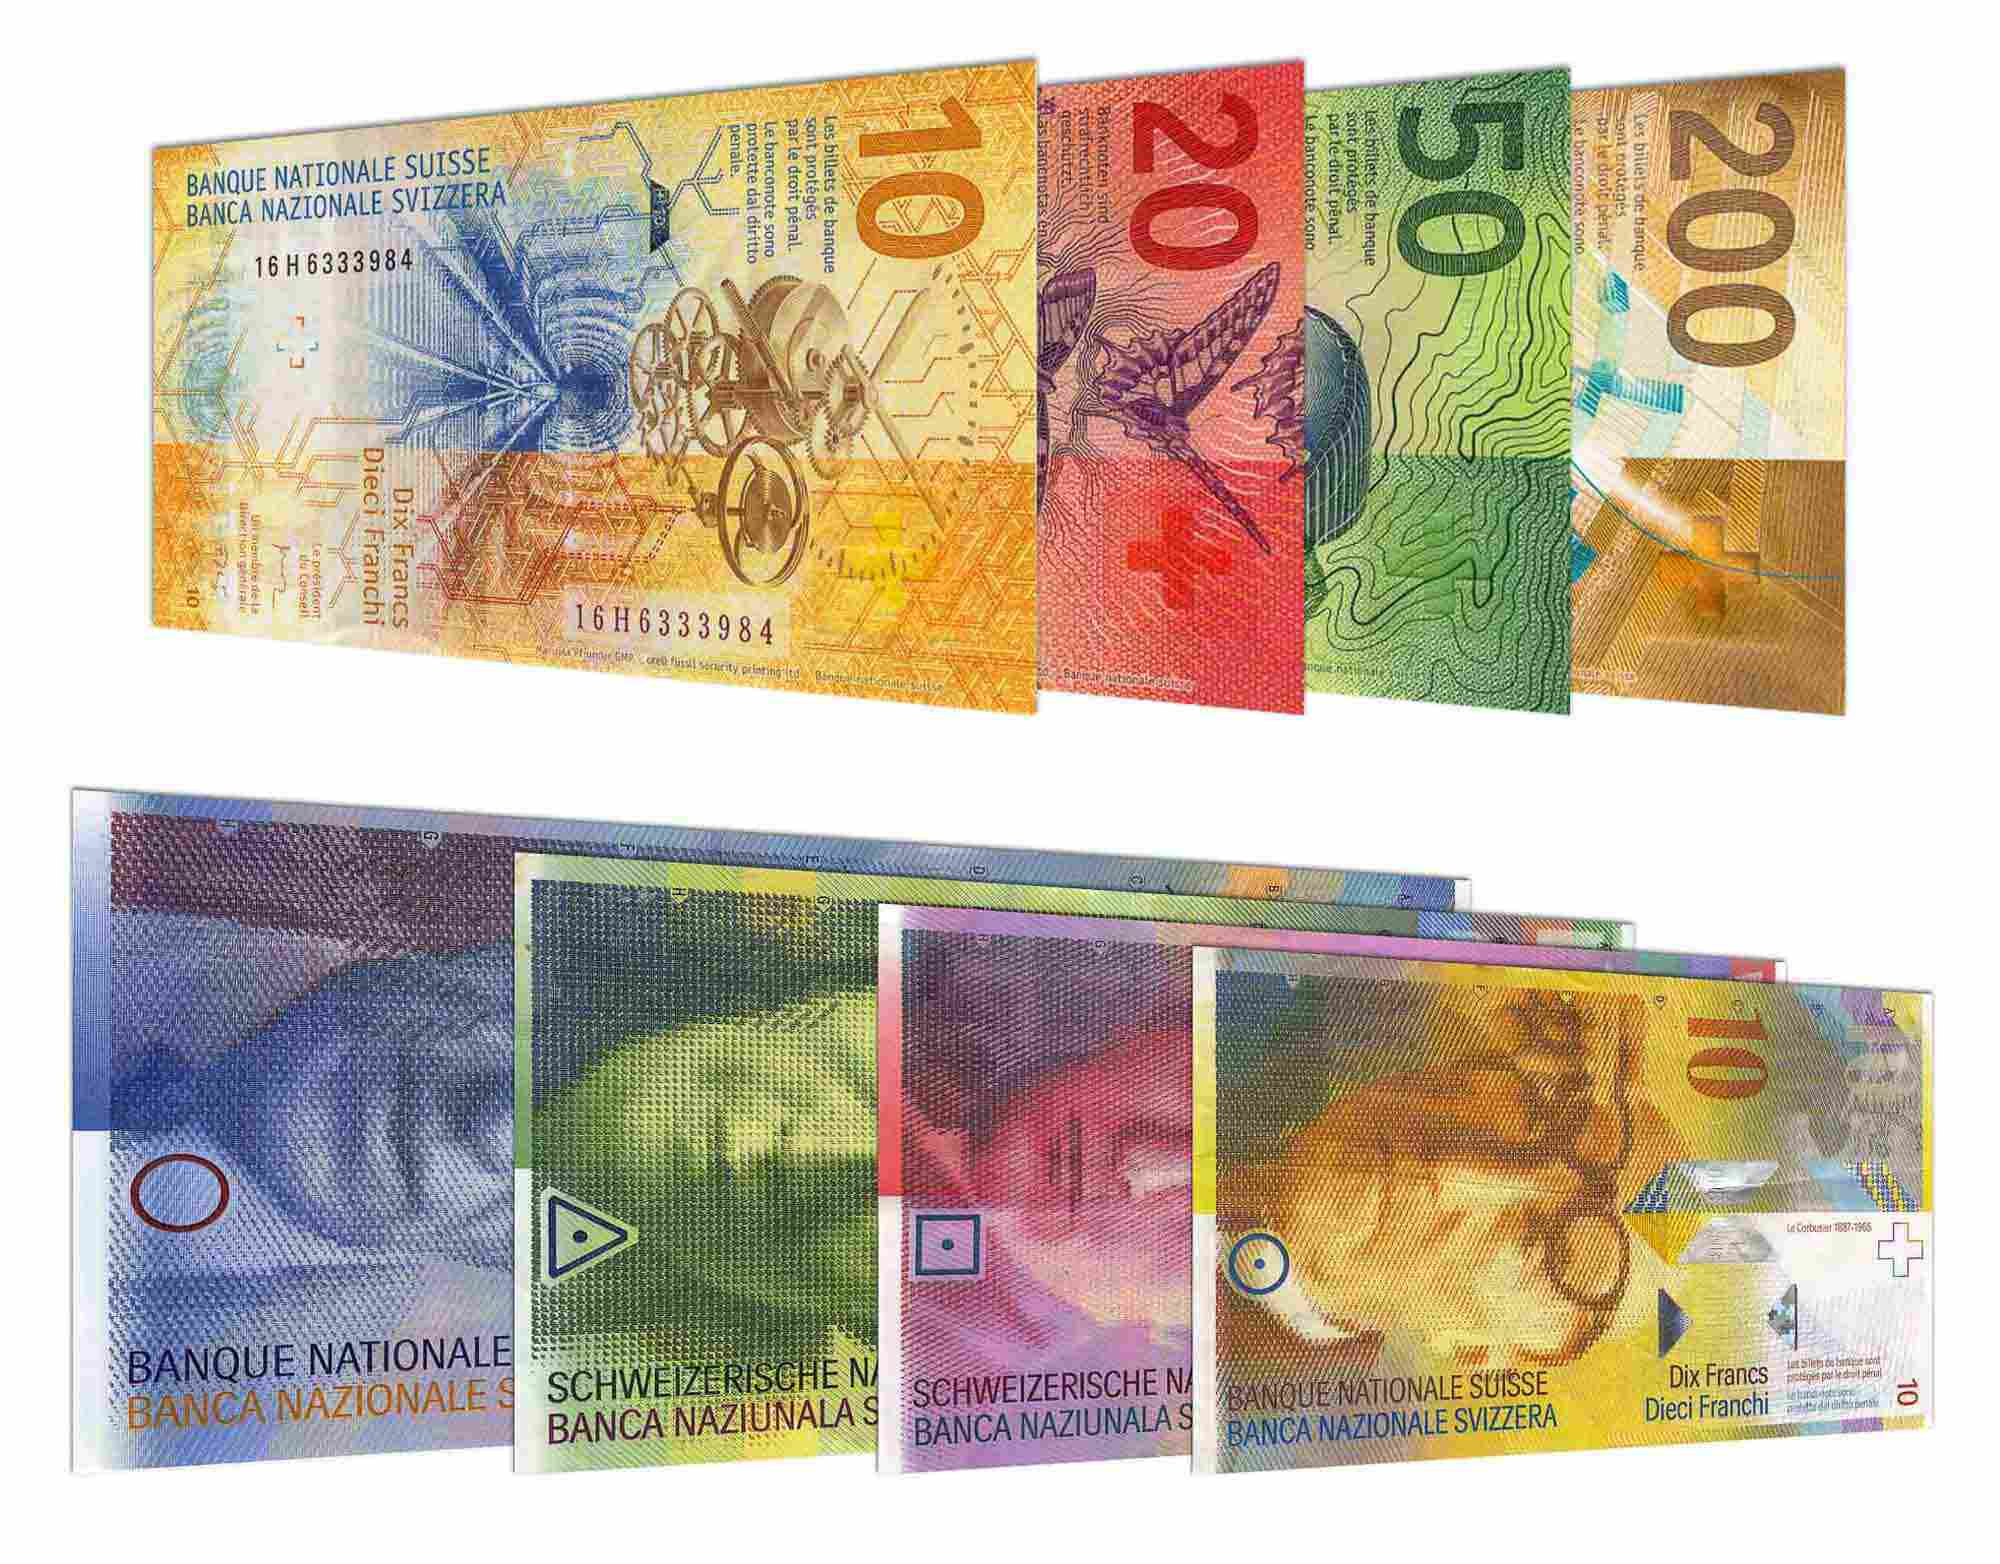
\includegraphics[max height=.45\textheight,
        max width=0.95\textwidth]{{Images/franc}.jpg}
    \end{center}
    \end{column}
    \end{columns}
}
\end{frame}
\begin{frame}[t]{Round 4 --- World Currencies --- \mbox{Answer 3}}
\vspace{-0.5em}
\begin{block}{Question}
Which country calls their currency's one- and two-dollar coins the ``Loonie'' and the ``Toonie'', respectively?
\end{block}

\visible<2->{
    \begin{columns}[T,totalwidth=\linewidth]
    \begin{column}{0.32\linewidth}
    \begin{block}{Answer}
    Canada
    \end{block}
    \end{column}
    \begin{column}{0.65\linewidth}
    \begin{center}
    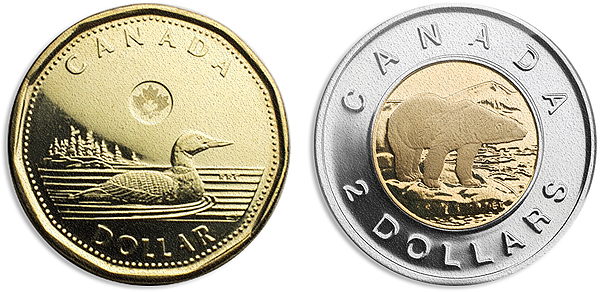
\includegraphics[max height=.45\textheight,
        max width=0.95\textwidth]{{Images/loonietoonie}.jpeg}
    \end{center}
    \end{column}
    \end{columns}
}
\end{frame}
\begin{frame}[t]{Round 4 --- World Currencies --- \mbox{Answer 4}}
\vspace{-0.5em}
\begin{block}{Question}
Which currency's three-letter code is MXN\@? (We need the country and the name of the currency.)
\end{block}

\visible<2->{
    \begin{columns}[T,totalwidth=\linewidth]
    \begin{column}{0.32\linewidth}
    \begin{block}{Answer}
    The Mexican peso
    \end{block}
    \end{column}
    \begin{column}{0.65\linewidth}
    \begin{center}
    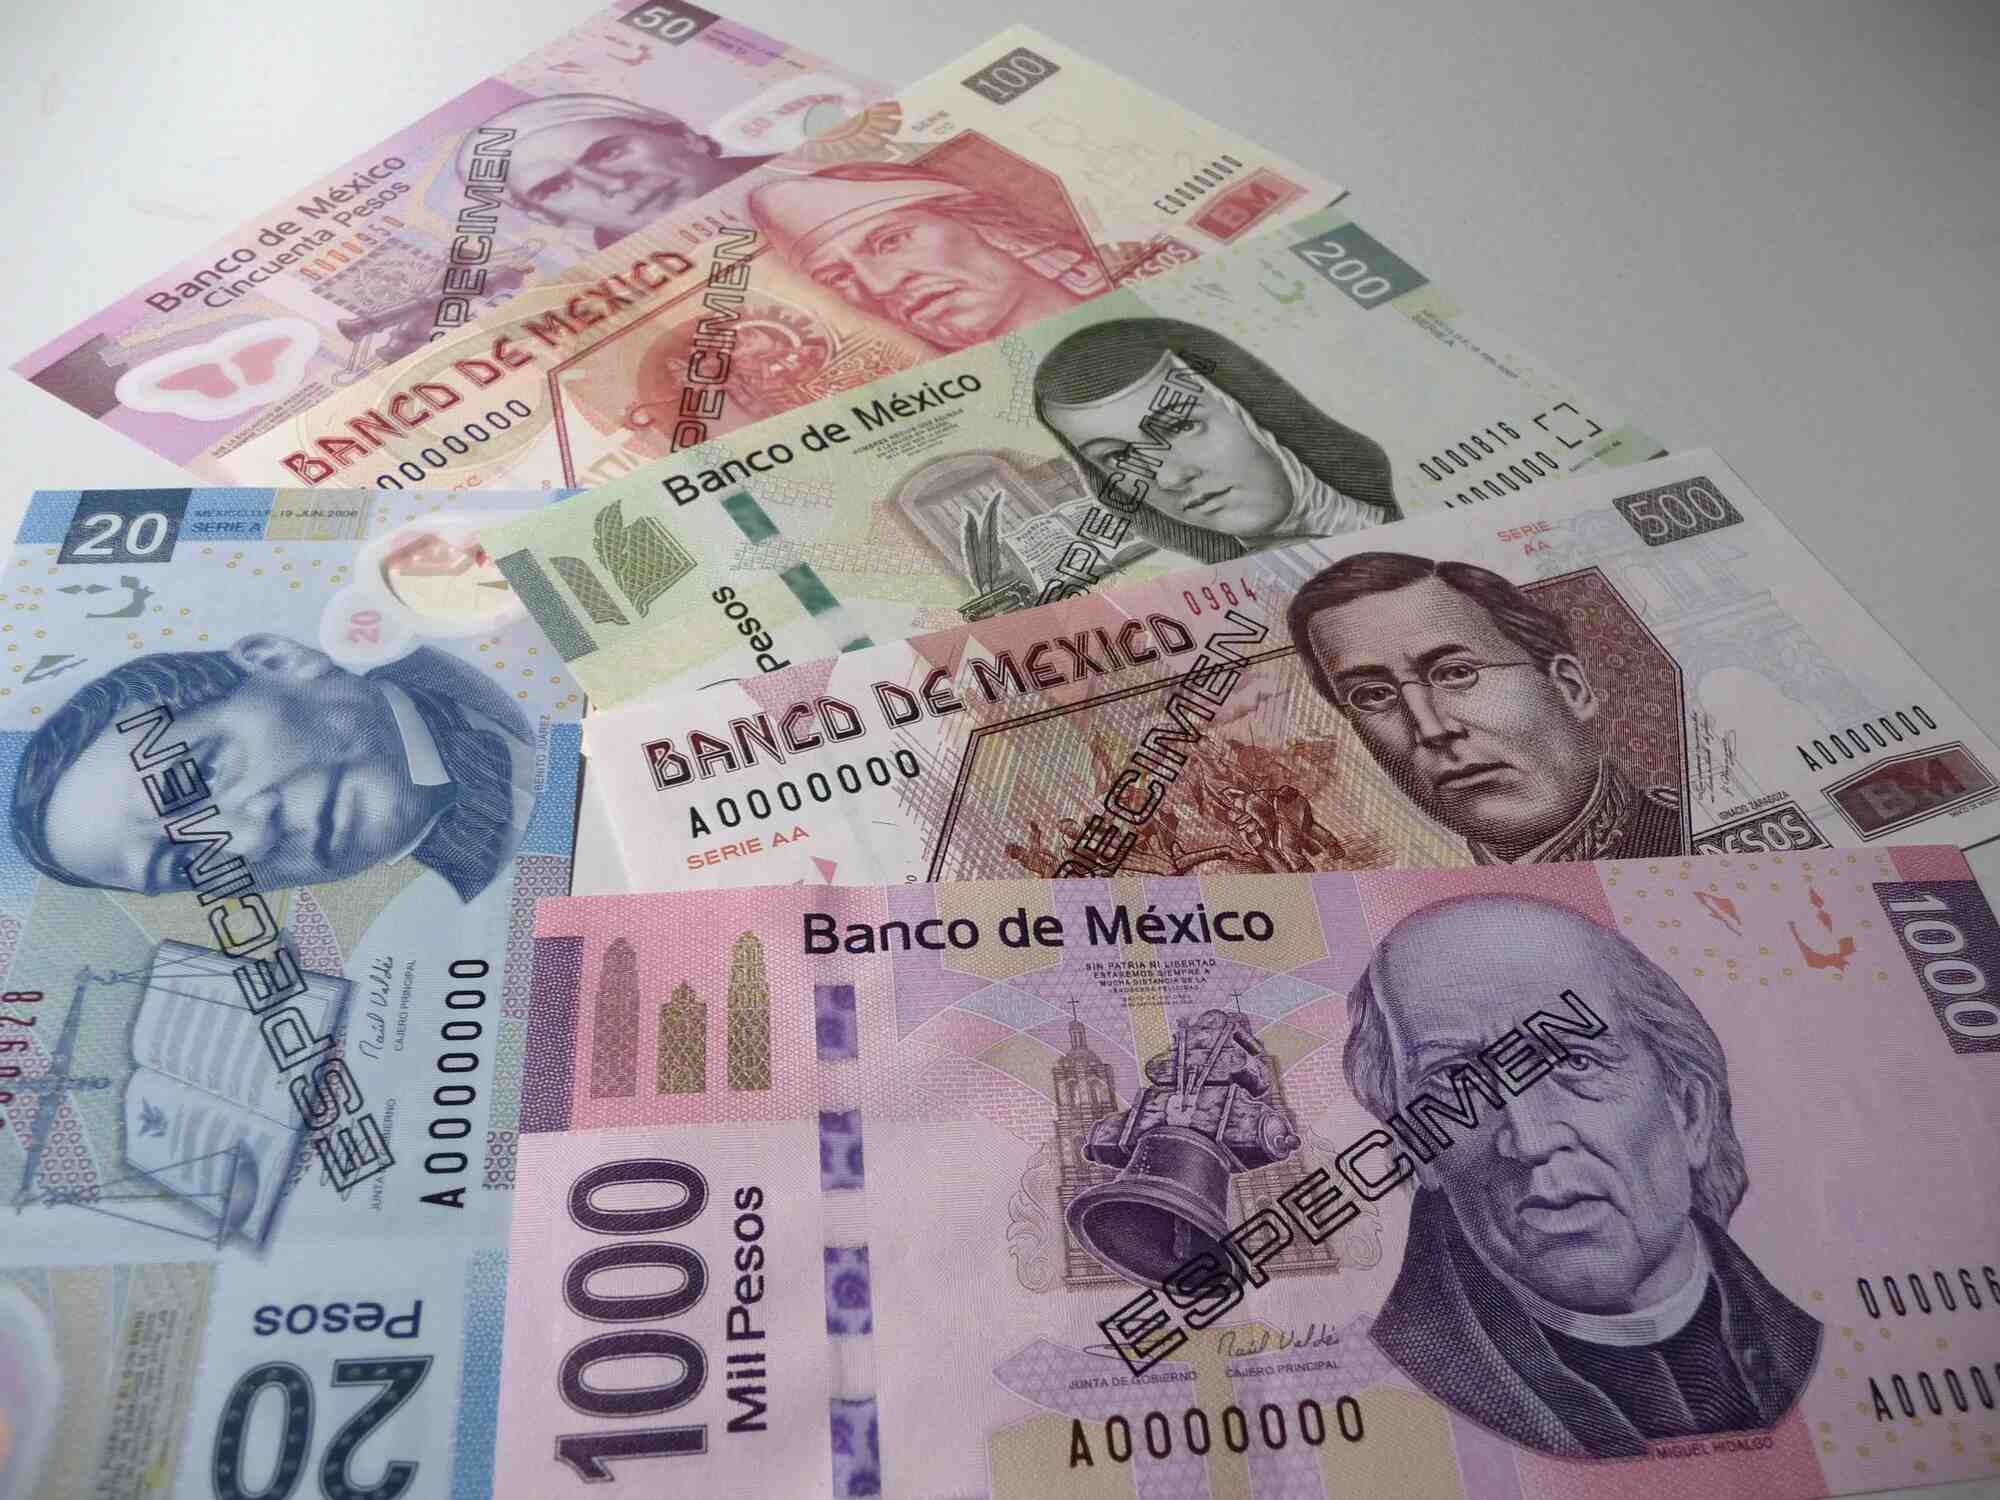
\includegraphics[max height=.45\textheight,
        max width=0.95\textwidth]{{Images/peso}.jpg}
    \end{center}
    \end{column}
    \end{columns}
}
\end{frame}
\begin{frame}[t]{Round 4 --- World Currencies --- \mbox{Answer 5}}
\vspace{-0.5em}
\begin{block}{Question}
What is the name of the currency that became widespread in early Islamic nations and is still used in several countries, including Algeria, Iraq, and Tunisia?
\end{block}

\visible<2->{
    \begin{columns}[T,totalwidth=\linewidth]
    \begin{column}{0.32\linewidth}
    \begin{block}{Answer}
    The dinar
    \end{block}
    \end{column}
    \begin{column}{0.65\linewidth}
    \begin{center}
    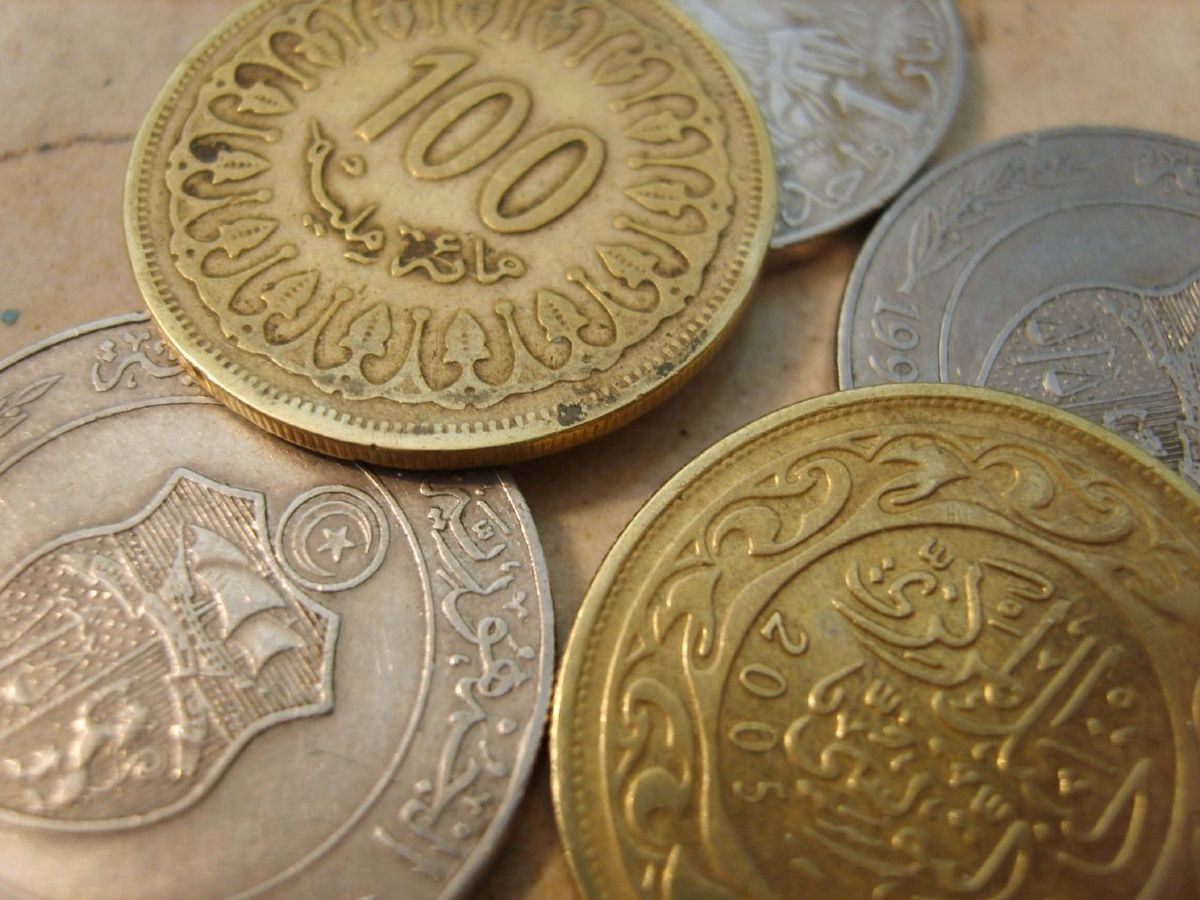
\includegraphics[max height=.45\textheight,
        max width=0.95\textwidth]{{Images/dinar}.jpg}
    \end{center}
    \end{column}
    \end{columns}
}
\end{frame}
\begin{frame}[t]{Round 4 --- World Currencies --- \mbox{Answer 6}}
\vspace{-0.5em}
\begin{block}{Question}
What is the world's oldest currency still in use?
\end{block}

\visible<2->{
    \begin{columns}[T,totalwidth=\linewidth]
    \begin{column}{0.32\linewidth}
    \begin{block}{Answer}
    The British pound / pound sterling / GBP
    \end{block}
    \end{column}
    \begin{column}{0.65\linewidth}
    \begin{center}
    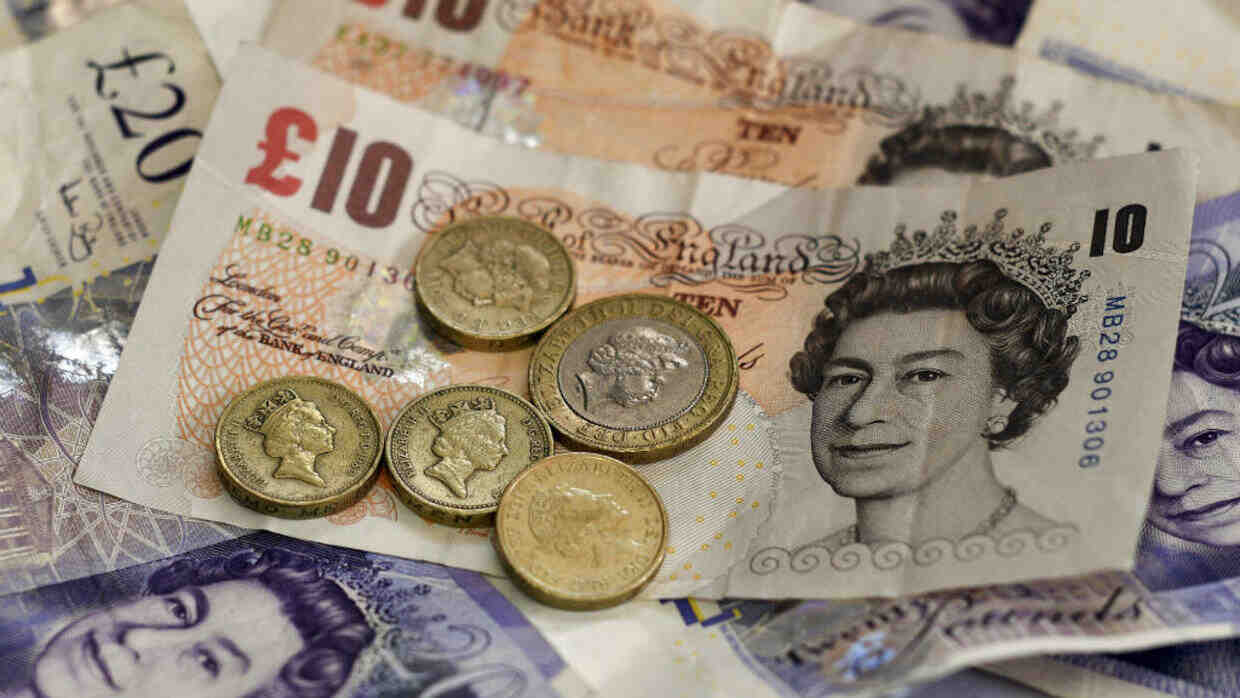
\includegraphics[max height=.45\textheight,
        max width=0.95\textwidth]{{Images/pound}.jpg}
    \end{center}
    \end{column}
    \end{columns}
}
\end{frame}
\begin{frame}[t]{Round 4 --- World Currencies --- \mbox{Answer 7}}
\vspace{-0.5em}
\begin{block}{Question}
Which country's currency was unpegged from the U.S. dollar in 2005, prior to which it had been fixed to trade at a ratio of 8.27:\$1?
\end{block}

\visible<2->{
    \begin{columns}[T,totalwidth=\linewidth]
    \begin{column}{0.32\linewidth}
    \begin{block}{Answer}
    China
    \end{block}
    \end{column}
    \begin{column}{0.65\linewidth}
    \begin{center}
    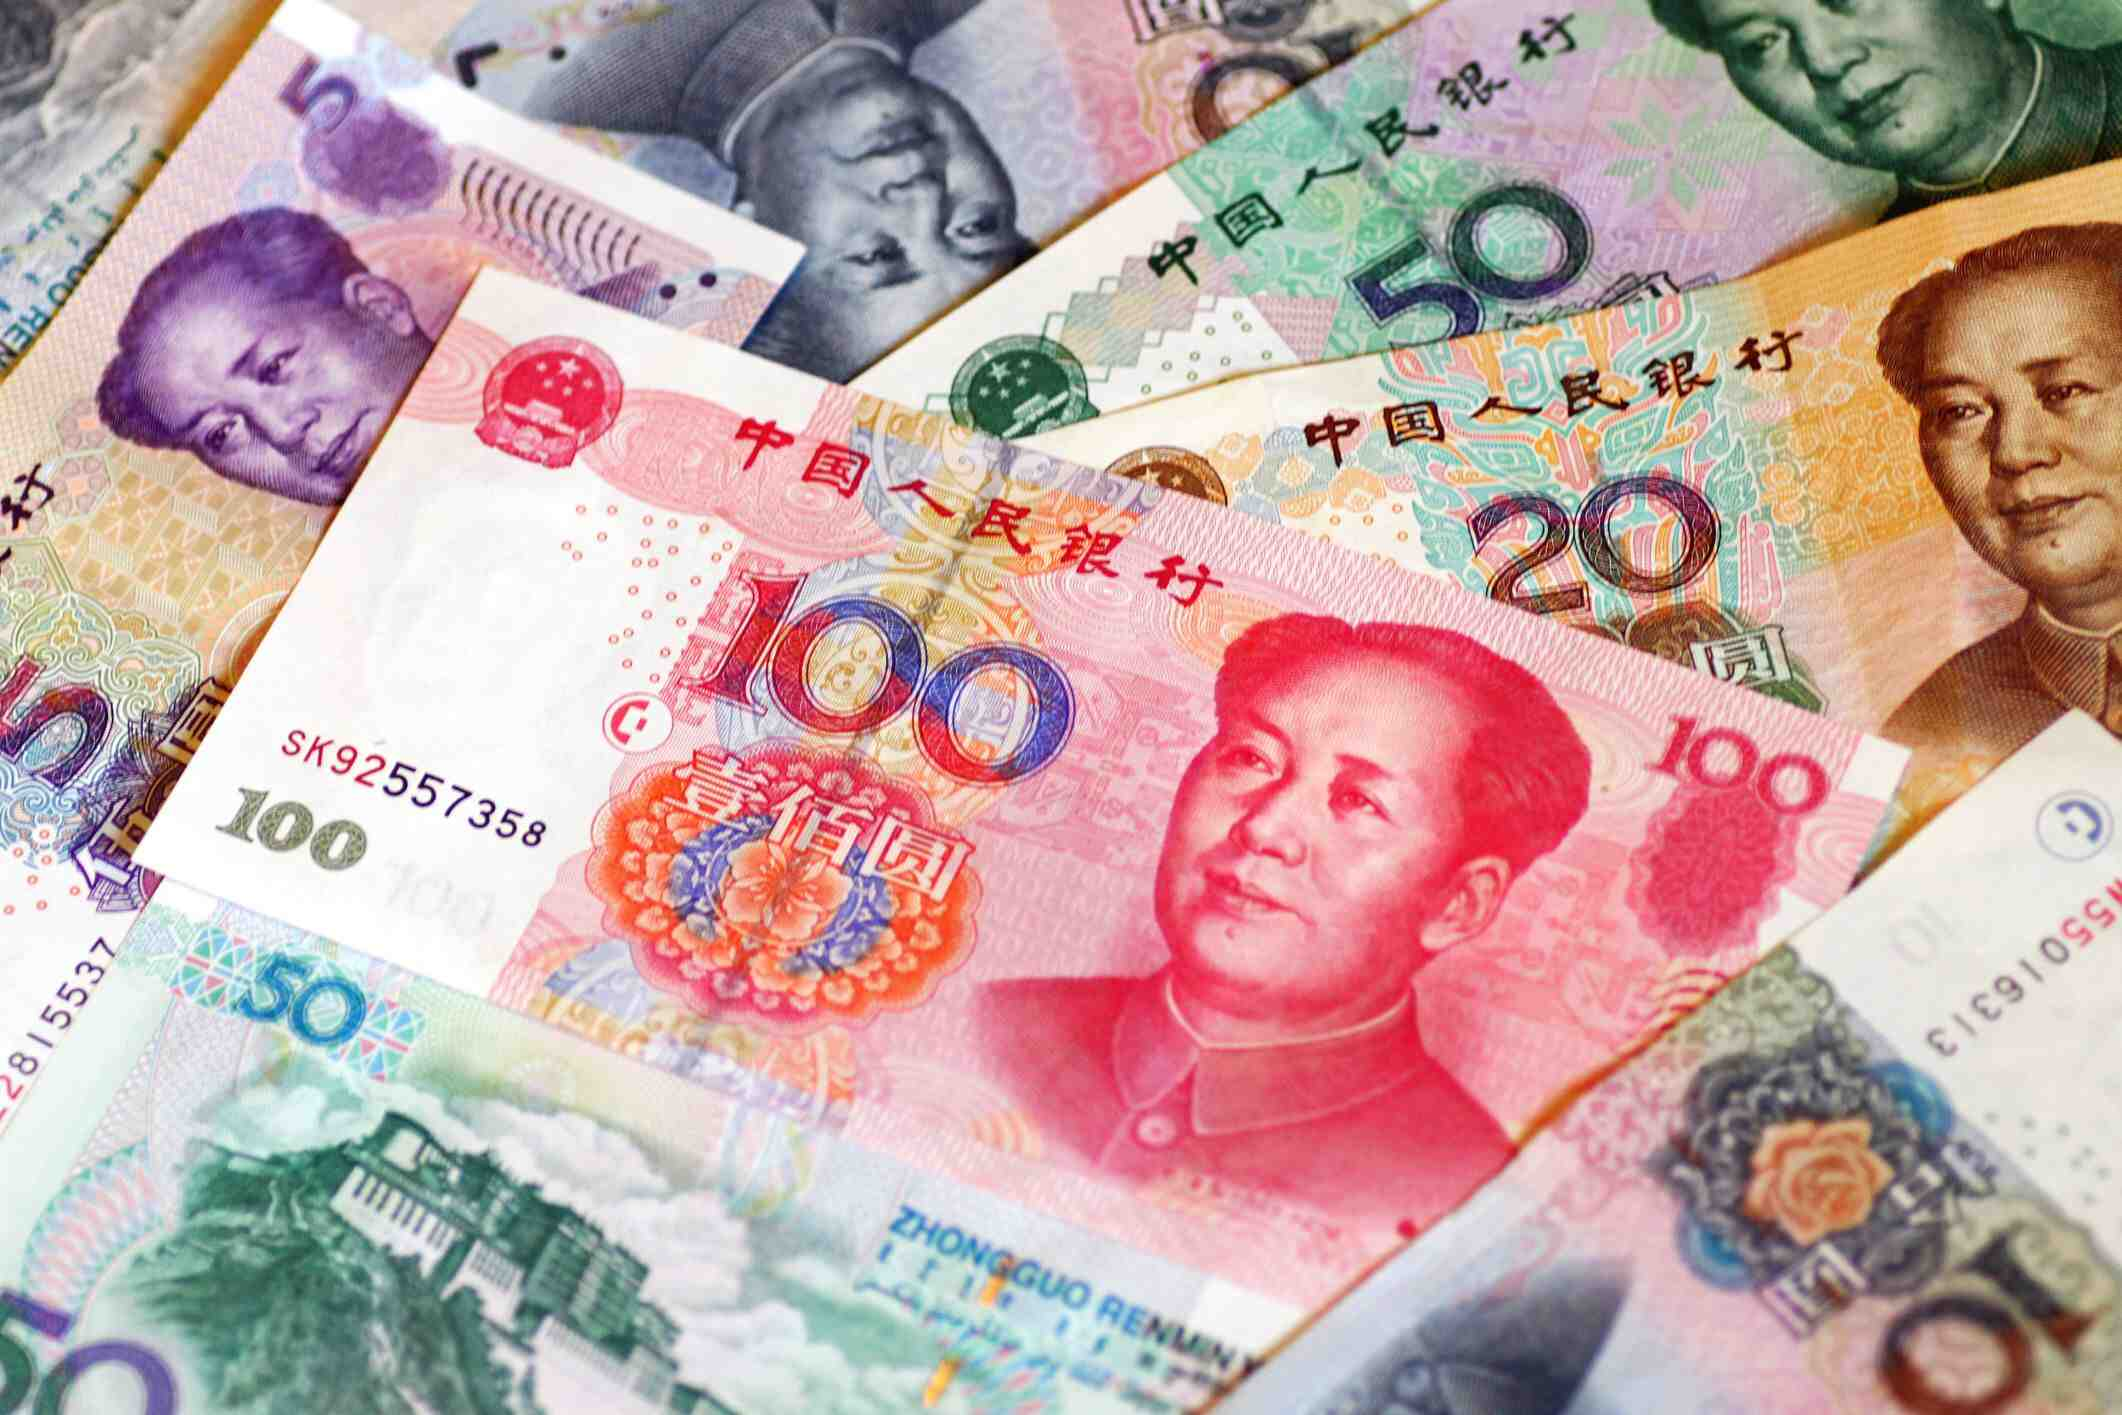
\includegraphics[max height=.45\textheight,
        max width=0.95\textwidth]{{Images/rmb}.jpg}
    \end{center}
    \end{column}
    \end{columns}
}
\end{frame}
\begin{frame}[t]{Round 4 --- World Currencies --- \mbox{Answer 8}}
\vspace{-0.5em}
\begin{columns}[T,totalwidth=\linewidth]
\begin{column}{0.32\linewidth}
\begin{block}{Question}
Which currency's symbol is pictured here? (We need the country and the name of the currency.)
\end{block}
\visible<2->{
    \begin{block}{Answer}
    The Indian rupee
    \end{block}
}
\end{column}
\begin{column}{0.65\linewidth}
\begin{center}

\includegraphics[max width=0.95\textwidth,max height=0.7\textheight]{{Images/rupee}.png}
\end{center}
\end{column}
\end{columns}
\end{frame}
\begin{frame}[t]{Round 4 --- World Currencies --- \mbox{Answer 9}}
\vspace{-0.5em}
\begin{block}{Question}
What is the name of the smallest unit of Bitcoin, which is worth one 100-millionth of a bitcoin?
\end{block}

\visible<2->{
    \begin{columns}[T,totalwidth=\linewidth]
    \begin{column}{0.32\linewidth}
    \begin{block}{Answer}
    A Satoshi
    \end{block}
    \end{column}
    \begin{column}{0.65\linewidth}
    \begin{center}
    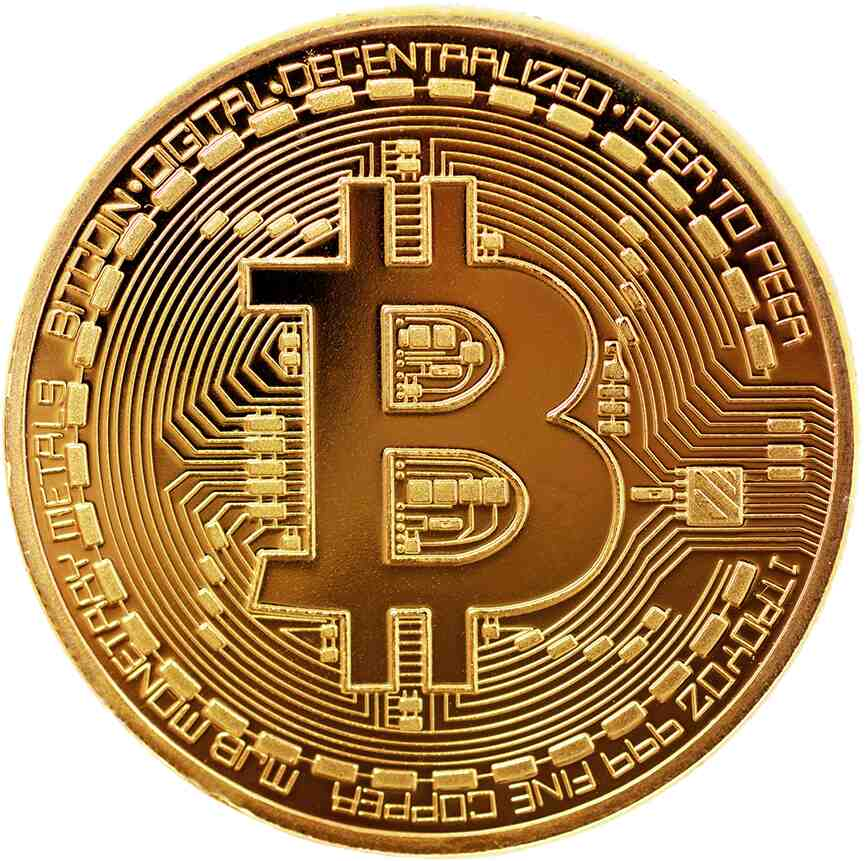
\includegraphics[max height=.45\textheight,
        max width=0.95\textwidth]{{Images/btc}.jpg}
    \end{center}
    \end{column}
    \end{columns}
}
\end{frame}
\begin{frame}[t]{Round 4 --- World Currencies --- \mbox{Answer 10}}
\vspace{-0.5em}
\begin{block}{Question}
What is the official currency of both Ecuador and El Salvador?
\end{block}

\visible<2->{
    \begin{columns}[T,totalwidth=\linewidth]
    \begin{column}{0.32\linewidth}
    \begin{block}{Answer}
    The U.S. dollar
    \end{block}
    \end{column}
    \begin{column}{0.65\linewidth}
    \begin{center}
    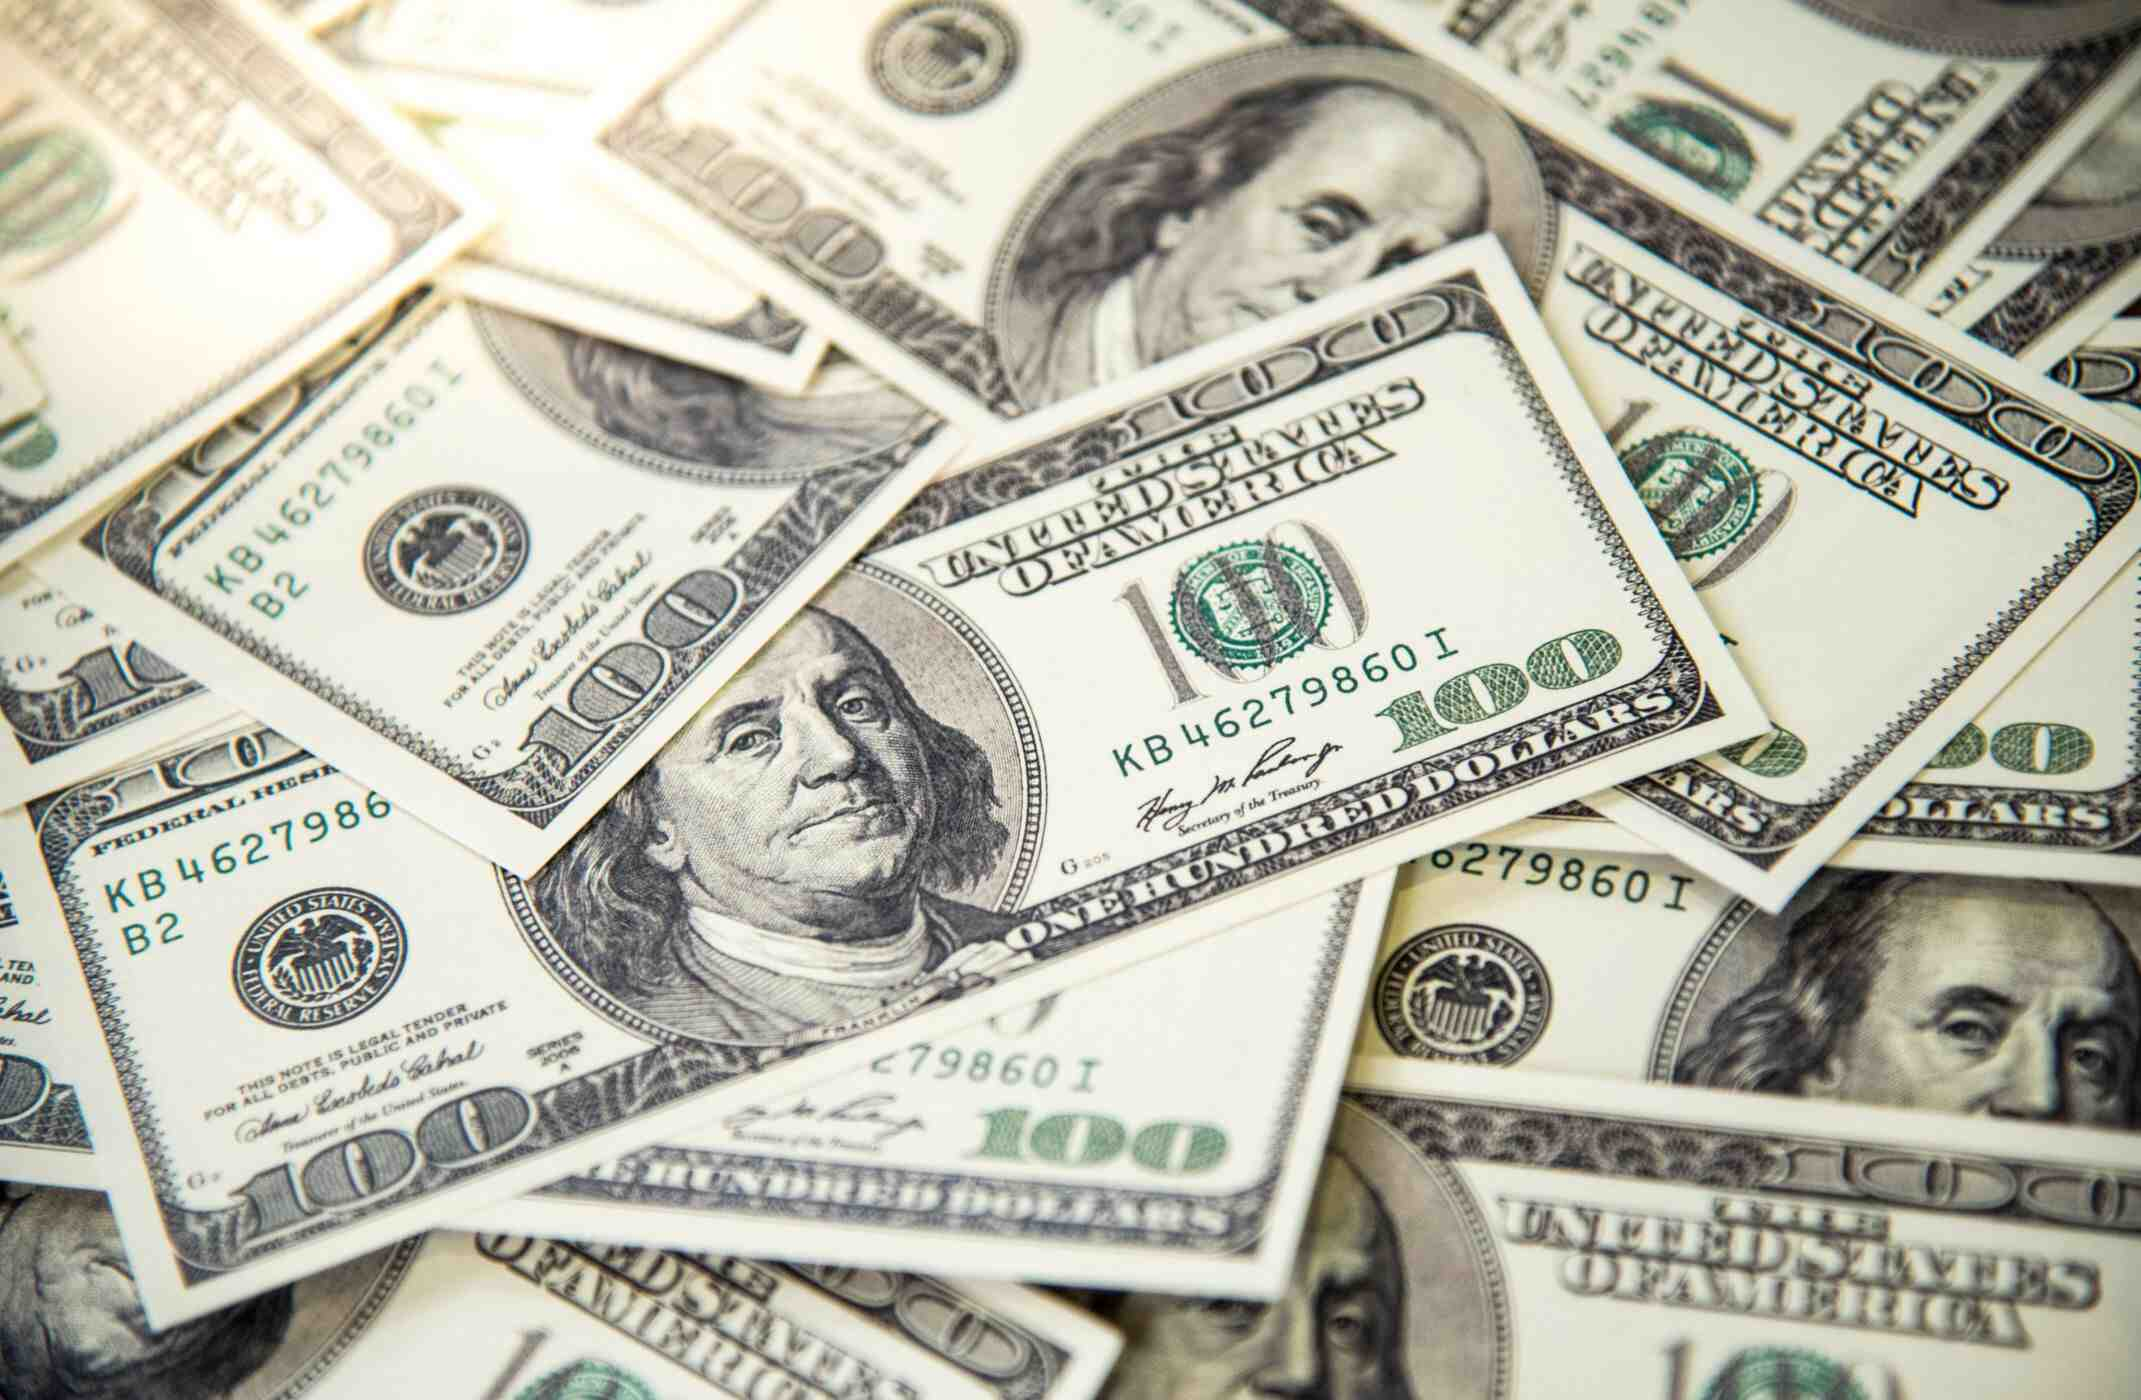
\includegraphics[max height=.45\textheight,
        max width=0.95\textwidth]{{Images/usd}.jpg}
    \end{center}
    \end{column}
    \end{columns}
}
\end{frame}
\def\thisSectionName{Transportation}
\section{Round 5}
\subsection*{Q1}
\begin{frame}[t]{Round 5 --- Transportation --- \mbox{Question 1}}
\vspace{-0.5em}
\begin{block}{Question}
What city had the world's first subway?  
\end{block}
\end{frame}
\subsection*{Q2}
\begin{frame}[t]{Round 5 --- Transportation --- \mbox{Question 2}}
\vspace{-0.5em}
\begin{block}{Question}
What were the names of the three ships sailed by Christopher Columbus and his crew on their 1492 voyage to the New World? (We need all three.)
\end{block}
\end{frame}
\subsection*{Q3}
\begin{frame}[t]{Round 5 --- Transportation --- \mbox{Question 3}}
\vspace{-0.5em}
\begin{block}{Question}
First flown in 1783, what kind of vehicle was the first to achieve sustained flight while carrying a person?
\end{block}
\end{frame}
\subsection*{Q4}
\begin{frame}[t]{Round 5 --- Transportation --- \mbox{Question 4}}
\vspace{-0.5em}
\begin{block}{Question}
The English name of what kind of boat comes from the Tamil word for ``logs bound together''?
\end{block}
\end{frame}
\subsection*{Q5}
\begin{frame}[t]{Round 5 --- Transportation --- \mbox{Question 5}}
\vspace{-0.5em}
\begin{block}{Question}
Which aircraft did Congress temporarily ban from landing in the U.S. due to concerns over the sonic booms it produced?
\end{block}
\end{frame}
\subsection*{Q6}
\begin{frame}[t]{Round 5 --- Transportation --- \mbox{Question 6}}
\vspace{-0.5em}
\begin{columns}[T,totalwidth=\linewidth]
\begin{column}{0.32\linewidth}
\begin{block}{Question}
What is the name for the specific type of early bicycle pictured here, with one large wheel in the front and one much smaller wheel in the back?
\end{block}
\end{column}
\begin{column}{0.65\linewidth}
\begin{center}
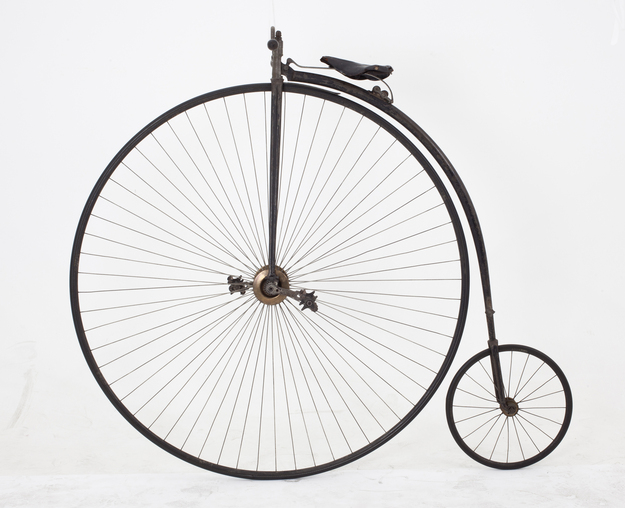
\includegraphics[max width=0.95\textwidth,max height=0.7\textheight]{{Images/pennyfarthing}.jpg}
\end{center}
\end{column}
\end{columns}
\end{frame}
\subsection*{Q7}
\begin{frame}[t]{Round 5 --- Transportation --- \mbox{Question 7}}
\vspace{-0.5em}
\begin{block}{Question}
What is the term for the distance between the rails of a railroad track?
\end{block}
\end{frame}
\subsection*{Q8}
\begin{frame}[t]{Round 5 --- Transportation --- \mbox{Question 8}}
\vspace{-0.5em}
\begin{block}{Question}
What is the name of the rocket that delivered the astronauts of the Apollo 11 program into outer space and which to this day remains the only launch vehicle to have carried humans beyond low Earth orbit?
\end{block}
\end{frame}
\subsection*{Q9}
\begin{frame}[t]{Round 5 --- Transportation --- \mbox{Question 9}}
\vspace{-0.5em}
\begin{block}{Question}
Who is the U.S. secretary of transportation under President Biden?
\end{block}
\end{frame}
\subsection*{Q10}
\begin{frame}[t]{Round 5 --- Transportation --- \mbox{Question 10}}
\vspace{-0.5em}
\begin{block}{Question}
The word ``cab'', as in taxi-cab and hansom cab, is short for the name of what type of horse-drawn vehicle?
\end{block}
\end{frame}
\subsection{Answers}
\begin{frame}[t]{Round 5 --- Transportation --- \mbox{Answer 1}}
\vspace{-0.5em}
\begin{block}{Question}
What city had the world's first subway?  
\end{block}

\visible<2->{
    \begin{columns}[T,totalwidth=\linewidth]
    \begin{column}{0.32\linewidth}
    \begin{block}{Answer}
    London (its Metropolitan Railway, founded in 1863, was the precursor to the Underground)
    \end{block}
    \end{column}
    \begin{column}{0.65\linewidth}
    \begin{center}
    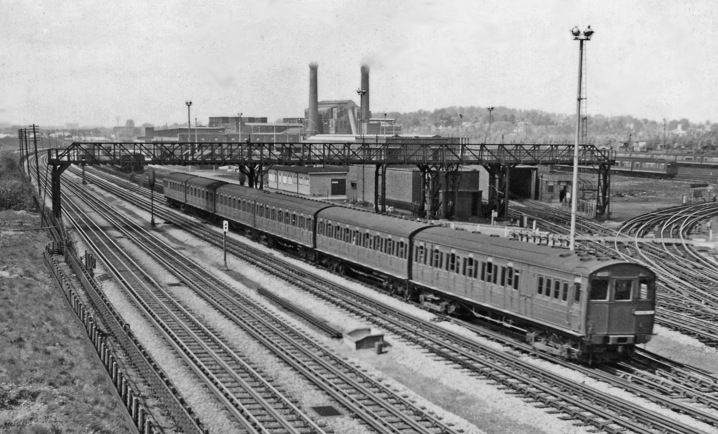
\includegraphics[max height=.45\textheight,
        max width=0.95\textwidth]{{Images/metrorailway}.jpg}
    \end{center}
    \end{column}
    \end{columns}
}
\end{frame}
\begin{frame}[t]{Round 5 --- Transportation --- \mbox{Answer 2}}
\vspace{-0.5em}
\begin{block}{Question}
What were the names of the three ships sailed by Christopher Columbus and his crew on their 1492 voyage to the New World? (We need all three.)
\end{block}

\visible<2->{
    \begin{columns}[T,totalwidth=\linewidth]
    \begin{column}{0.32\linewidth}
    \begin{block}{Answer}
    The \emph{Ni{\~n}a} (whose official name was \emph{Santa Clara}), the \emph{Pinta}, and the \emph{Santa Maria}
    \end{block}
    \end{column}
    \begin{column}{0.65\linewidth}
    \begin{center}
    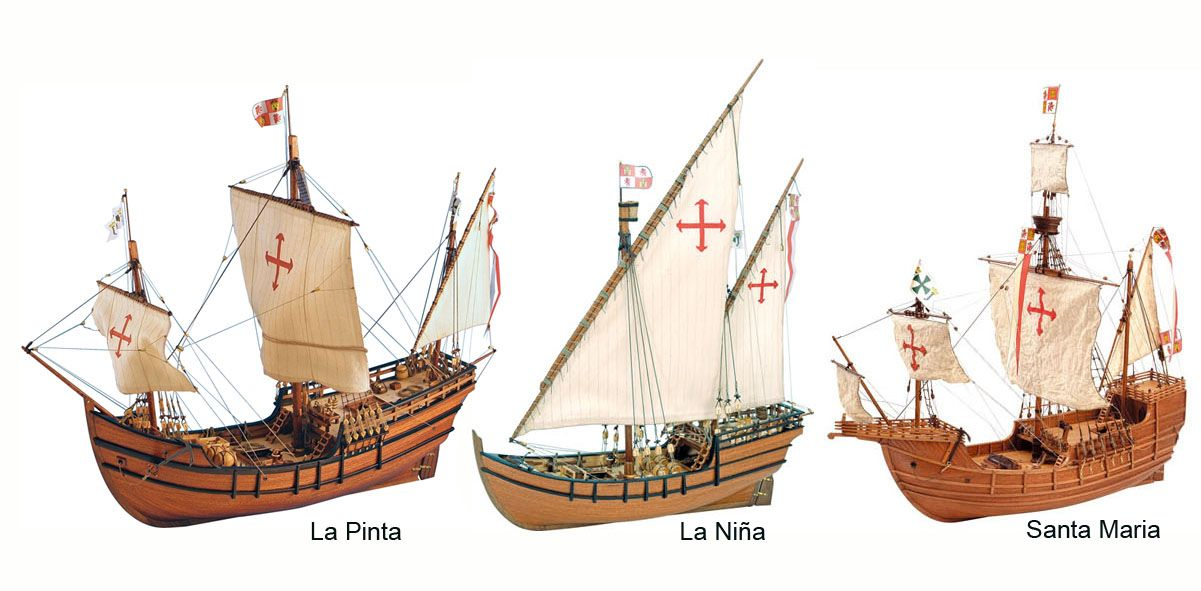
\includegraphics[max height=.45\textheight,
        max width=0.95\textwidth]{{Images/colombus}.jpg}
    \end{center}
    \end{column}
    \end{columns}
}
\end{frame}
\begin{frame}[t]{Round 5 --- Transportation --- \mbox{Answer 3}}
\vspace{-0.5em}
\begin{block}{Question}
First flown in 1783, what kind of vehicle was the first to achieve sustained flight while carrying a person?
\end{block}

\visible<2->{
    \begin{columns}[T,totalwidth=\linewidth]
    \begin{column}{0.32\linewidth}
    \begin{block}{Answer}
    A hot air balloon
    \end{block}
    \end{column}
    \begin{column}{0.65\linewidth}
    \begin{center}
    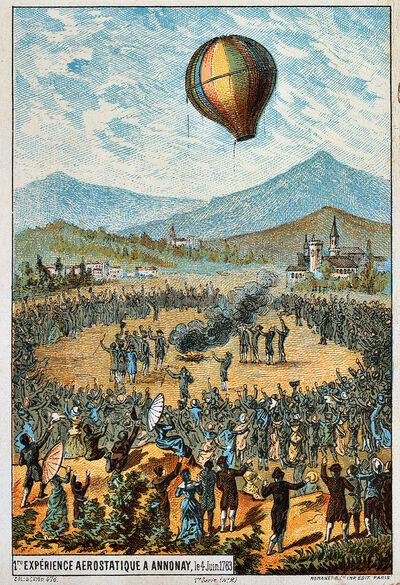
\includegraphics[max height=.45\textheight,
        max width=0.95\textwidth]{{Images/hotair}.jpg}
    \end{center}
    \end{column}
    \end{columns}
}
\end{frame}
\begin{frame}[t]{Round 5 --- Transportation --- \mbox{Answer 4}}
\vspace{-0.5em}
\begin{block}{Question}
The English name of what kind of boat comes from the Tamil word for ``logs bound together''?
\end{block}

\visible<2->{
    \begin{columns}[T,totalwidth=\linewidth]
    \begin{column}{0.32\linewidth}
    \begin{block}{Answer}
    Catamaran
    \end{block}
    \end{column}
    \begin{column}{0.65\linewidth}
    \begin{center}
    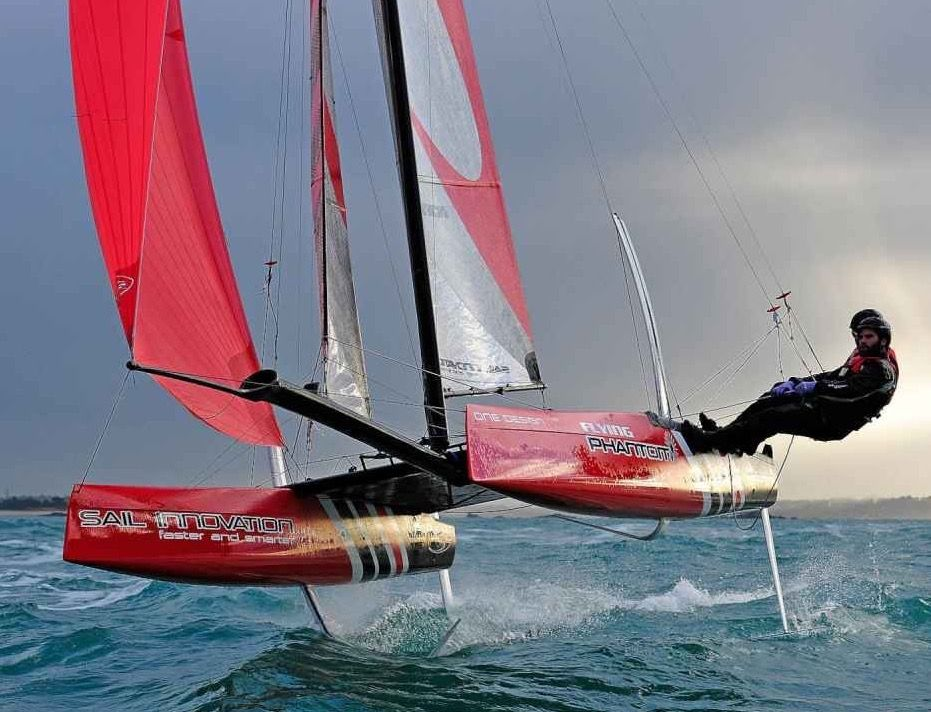
\includegraphics[max height=.45\textheight,
        max width=0.95\textwidth]{{Images/catamaran}.jpg}
    \end{center}
    \end{column}
    \end{columns}
}
\end{frame}
\begin{frame}[t]{Round 5 --- Transportation --- \mbox{Answer 5}}
\vspace{-0.5em}
\begin{block}{Question}
Which aircraft did Congress temporarily ban from landing in the U.S. due to concerns over the sonic booms it produced?
\end{block}

\visible<2->{
    \begin{columns}[T,totalwidth=\linewidth]
    \begin{column}{0.32\linewidth}
    \begin{block}{Answer}
    The Concorde
    \end{block}
    \end{column}
    \begin{column}{0.65\linewidth}
    \begin{center}
    \includegraphics[max height=.45\textheight,
        max width=0.95\textwidth]{{Images/concorde}.jpeg}
    \end{center}
    \end{column}
    \end{columns}
}
\end{frame}
\begin{frame}[t]{Round 5 --- Transportation --- \mbox{Answer 6}}
\vspace{-0.5em}
\begin{columns}[T,totalwidth=\linewidth]
\begin{column}{0.32\linewidth}
\begin{block}{Question}
What is the name for the specific type of early bicycle pictured here, with one large wheel in the front and one much smaller wheel in the back?
\end{block}
\visible<2->{
    \begin{block}{Answer}
    Penny-farthing, high-wheeler, or ``ordinary''
    \end{block}
}
\end{column}
\begin{column}{0.65\linewidth}
\begin{center}
\includegraphics[max width=0.95\textwidth,max height=0.7\textheight]{{Images/pennyfarthing}.jpg}
\end{center}
\end{column}
\end{columns}
\end{frame}
\begin{frame}[t]{Round 5 --- Transportation --- \mbox{Answer 7}}
\vspace{-0.5em}
\begin{block}{Question}
What is the term for the distance between the rails of a railroad track?
\end{block}

\visible<2->{
    \begin{columns}[T,totalwidth=\linewidth]
    \begin{column}{0.32\linewidth}
    \begin{block}{Answer}
    Gauge / gage
    \end{block}
    \end{column}
    \begin{column}{0.65\linewidth}
    \begin{center}
    \includegraphics[max height=.45\textheight,
        max width=0.95\textwidth]{{Images/gauge}.png}
    \end{center}
    \end{column}
    \end{columns}
}
\end{frame}
\begin{frame}[t]{Round 5 --- Transportation --- \mbox{Answer 8}}
\vspace{-0.5em}
\begin{block}{Question}
What is the name of the rocket that delivered the astronauts of the Apollo 11 program into outer space and which to this day remains the only launch vehicle to have carried humans beyond low Earth orbit?
\end{block}

\visible<2->{
    \begin{columns}[T,totalwidth=\linewidth]
    \begin{column}{0.32\linewidth}
    \begin{block}{Answer}
    Saturn V
    \end{block}
    \end{column}
    \begin{column}{0.65\linewidth}
    \begin{center}
    \includegraphics[max height=.45\textheight,
        max width=0.95\textwidth]{{Images/saturnV}.jpg}
    \end{center}
    \end{column}
    \end{columns}
}
\end{frame}
\begin{frame}[t]{Round 5 --- Transportation --- \mbox{Answer 9}}
\vspace{-0.5em}
\begin{block}{Question}
Who is the U.S. secretary of transportation under President Biden?
\end{block}

\visible<2->{
    \begin{columns}[T,totalwidth=\linewidth]
    \begin{column}{0.32\linewidth}
    \begin{block}{Answer}
    Pete Buttigieg
    \end{block}
    \end{column}
    \begin{column}{0.65\linewidth}
    \begin{center}
    \includegraphics[max height=.45\textheight,
        max width=0.95\textwidth]{{Images/pete}.jpg}
    \end{center}
    \end{column}
    \end{columns}
}
\end{frame}
\begin{frame}[t]{Round 5 --- Transportation --- \mbox{Answer 10}}
\vspace{-0.5em}
\begin{block}{Question}
The word ``cab'', as in taxi-cab and hansom cab, is short for the name of what type of horse-drawn vehicle?
\end{block}

\visible<2->{
    \begin{columns}[T,totalwidth=\linewidth]
    \begin{column}{0.32\linewidth}
    \begin{block}{Answer}
    A cabriolet (a two-wheeled horse-drawn carriage with a folding roof)
    \end{block}
    \end{column}
    \begin{column}{0.65\linewidth}
    \begin{center}
    \includegraphics[max height=.45\textheight,
        max width=0.95\textwidth]{{Images/cab}.jpg}
    \end{center}
    \end{column}
    \end{columns}
}
\end{frame}
\def\thisSectionName{Swindlers, Frauds, and Cheats}
\section{Round 6}
\subsection*{Q1}
\begin{frame}[t]{Round 6 --- Swindlers, Frauds, and Cheats --- \mbox{Question 1}}
\vspace{-0.5em}
\begin{block}{Question}
The 2002 biographical film \emph{Catch Me If You Can} was about which real-life conman who committed check fraud and impersonated a pilot, a doctor, and a lawyer before being arrested at the age of 21?
\end{block}
\end{frame}
\subsection*{Q2}
\begin{frame}[t]{Round 6 --- Swindlers, Frauds, and Cheats --- \mbox{Question 2}}
\vspace{-0.5em}
\begin{columns}[T,totalwidth=\linewidth]
\begin{column}{0.32\linewidth}
\begin{block}{Question}
The professional baseball player pictured here was the mastermind of what game-fixing scandal in Major League Baseball?
\end{block}
\end{column}
\begin{column}{0.65\linewidth}
\begin{center}
\includegraphics[max width=0.95\textwidth,max height=0.7\textheight]{{Images/whitesox}.jpg}
\end{center}
\end{column}
\end{columns}
\end{frame}
\subsection*{Q3}
\begin{frame}[t]{Round 6 --- Swindlers, Frauds, and Cheats --- \mbox{Question 3}}
\vspace{-0.5em}
\begin{block}{Question}
Which alleged fraudster, whose trial on charges of wire fraud and conspiracy to commit wire fraud is set to begin in July of this year, is the subject of the book \emph{Bad Blood}?
\end{block}
\end{frame}
\subsection*{Q4}
\begin{frame}[t]{Round 6 --- Swindlers, Frauds, and Cheats --- \mbox{Question 4}}
\vspace{-0.5em}
\begin{block}{Question}
George C. Parker became known for the phrase ``I have a bridge to sell you'' thanks to his repeated success in fraudulently selling which New York City landmark to unwitting buyers?
\end{block}
\end{frame}
\subsection*{Q5}
\begin{frame}[t]{Round 6 --- Swindlers, Frauds, and Cheats --- \mbox{Question 5}}
\vspace{-0.5em}
\begin{block}{Question}
In 1973, which illusionist and self-proclaimed psychic appeared on \emph{The Tonight Show}, but was unable to reproduce his effects because Johnny Carson had replaced his magic props with fakes?
\end{block}
\end{frame}
\subsection*{Q6}
\begin{frame}[t]{Round 6 --- Swindlers, Frauds, and Cheats --- \mbox{Question 6}}
\vspace{-0.5em}
\begin{block}{Question}
From start to finish, Charles Ponzi's eponymous scheme only lasted about seven months. To within five years, in what year did it take place?
\end{block}
\end{frame}
\subsection*{Q7}
\begin{frame}[t]{Round 6 --- Swindlers, Frauds, and Cheats --- \mbox{Question 7}}
\vspace{-0.5em}
\begin{block}{Question}
Which NFL player orchestrated the ``Deflategate'' incident, in which he had his team's footballs deflated below regulation pressure?
\end{block}
\end{frame}
\subsection*{Q8}
\begin{frame}[t]{Round 6 --- Swindlers, Frauds, and Cheats --- \mbox{Question 8}}
\vspace{-0.5em}
\begin{block}{Question}
Which televangelist built Heritage USA, a Christian-themed amusement park, and was subsequently convicted of financial fraud for selling more memberships to the amusement park than there was capacity for?
\end{block}
\end{frame}
\subsection*{Q9}
\begin{frame}[t]{Round 6 --- Swindlers, Frauds, and Cheats --- \mbox{Question 9}}
\vspace{-0.5em}
\begin{block}{Question}
The Houston Astros cheated during the 2017 and 2018 baseball seasons by performing what illegal action with the help of cameras and other technology?
\end{block}
\end{frame}
\subsection*{Q10}
\begin{frame}[t]{Round 6 --- Swindlers, Frauds, and Cheats --- \mbox{Question 10}}
\vspace{-0.5em}
\begin{block}{Question}
What was the title of the fictional musical in Mel Brooks's \emph{The Producers} that was designed to flop so that its producers could pocket all of the money invested into it?
\end{block}
\end{frame}
\subsection{Answers}
\begin{frame}[t]{Round 6 --- Swindlers, Frauds, and Cheats --- \mbox{Answer 1}}
\vspace{-0.5em}
\begin{block}{Question}
The 2002 biographical film \emph{Catch Me If You Can} was about which real-life conman who committed check fraud and impersonated a pilot, a doctor, and a lawyer before being arrested at the age of 21?
\end{block}

\visible<2->{
    \begin{columns}[T,totalwidth=\linewidth]
    \begin{column}{0.32\linewidth}
    \begin{block}{Answer}
    Frank Abagnale Jr.\ (without the ``Jr.'' is fine)
    \end{block}
    \end{column}
    \begin{column}{0.65\linewidth}
    \begin{center}
    \includegraphics[max height=.45\textheight,
        max width=0.95\textwidth]{{Images/abagnale}.jpeg}
    \end{center}
    \end{column}
    \end{columns}
}
\end{frame}
\begin{frame}[t]{Round 6 --- Swindlers, Frauds, and Cheats --- \mbox{Answer 2}}
\vspace{-0.5em}
\begin{columns}[T,totalwidth=\linewidth]
\begin{column}{0.32\linewidth}
\begin{block}{Question}
The professional baseball player pictured here was the mastermind of what game-fixing scandal in Major League Baseball?
\end{block}
\visible<2->{
    \begin{block}{Answer}
    The Black Sox Scandal
    \end{block}
}
\end{column}
\begin{column}{0.65\linewidth}
\begin{center}
\includegraphics[max width=0.95\textwidth,max height=0.7\textheight]{{Images/whitesox}.jpg}
\end{center}
\end{column}
\end{columns}
\end{frame}
\begin{frame}[t]{Round 6 --- Swindlers, Frauds, and Cheats --- \mbox{Answer 3}}
\vspace{-0.5em}
\begin{block}{Question}
Which alleged fraudster, whose trial on charges of wire fraud and conspiracy to commit wire fraud is set to begin in July of this year, is the subject of the book \emph{Bad Blood}?
\end{block}

\visible<2->{
    \begin{columns}[T,totalwidth=\linewidth]
    \begin{column}{0.32\linewidth}
    \begin{block}{Answer}
    Elizabeth Holmes
    \end{block}
    \end{column}
    \begin{column}{0.65\linewidth}
    \begin{center}
    \includegraphics[max height=.45\textheight,
        max width=0.95\textwidth]{{Images/holmes}.jpg}
    \end{center}
    \end{column}
    \end{columns}
}
\end{frame}
\begin{frame}[t]{Round 6 --- Swindlers, Frauds, and Cheats --- \mbox{Answer 4}}
\vspace{-0.5em}
\begin{block}{Question}
George C. Parker became known for the phrase ``I have a bridge to sell you'' thanks to his repeated success in fraudulently selling which New York City landmark to unwitting buyers?
\end{block}

\visible<2->{
    \begin{columns}[T,totalwidth=\linewidth]
    \begin{column}{0.32\linewidth}
    \begin{block}{Answer}
    The Brooklyn Bridge
    \end{block}
    \end{column}
    \begin{column}{0.65\linewidth}
    \begin{center}
    \includegraphics[max height=.45\textheight,
        max width=0.95\textwidth]{{Images/bridge}.jpg}
    \end{center}
    \end{column}
    \end{columns}
}
\end{frame}
\begin{frame}[t]{Round 6 --- Swindlers, Frauds, and Cheats --- \mbox{Answer 5}}
\vspace{-0.5em}
\begin{block}{Question}
In 1973, which illusionist and self-proclaimed psychic appeared on \emph{The Tonight Show}, but was unable to reproduce his effects because Johnny Carson had replaced his magic props with fakes?
\end{block}

\visible<2->{
    \begin{columns}[T,totalwidth=\linewidth]
    \begin{column}{0.32\linewidth}
    \begin{block}{Answer}
    Uri Geller
    \end{block}
    \end{column}
    \begin{column}{0.65\linewidth}
    \begin{center}
    \includegraphics[max height=.45\textheight,
        max width=0.95\textwidth]{{Images/geller}.jpg}
    \end{center}
    \end{column}
    \end{columns}
}
\end{frame}
\begin{frame}[t]{Round 6 --- Swindlers, Frauds, and Cheats --- \mbox{Answer 6}}
\vspace{-0.5em}
\begin{block}{Question}
From start to finish, Charles Ponzi's eponymous scheme only lasted about seven months. To within five years, in what year did it take place?
\end{block}

\visible<2->{
    \begin{columns}[T,totalwidth=\linewidth]
    \begin{column}{0.32\linewidth}
    \begin{block}{Answer}
    1920 (1915--1925 will be accepted)
    \end{block}
    \end{column}
    \begin{column}{0.65\linewidth}
    \begin{center}
    \includegraphics[max height=.45\textheight,
        max width=0.95\textwidth]{{Images/ponzi}.jpg}
    \end{center}
    \end{column}
    \end{columns}
}
\end{frame}
\begin{frame}[t]{Round 6 --- Swindlers, Frauds, and Cheats --- \mbox{Answer 7}}
\vspace{-0.5em}
\begin{block}{Question}
Which NFL player orchestrated the ``Deflategate'' incident, in which he had his team's footballs deflated below regulation pressure?
\end{block}

\visible<2->{
    \begin{columns}[T,totalwidth=\linewidth]
    \begin{column}{0.32\linewidth}
    \begin{block}{Answer}
    Tom Brady
    \end{block}
    \end{column}
    \begin{column}{0.65\linewidth}
    \begin{center}
    \includegraphics[max height=.45\textheight,
        max width=0.95\textwidth]{{Images/brady}.jpg}
    \end{center}
    \end{column}
    \end{columns}
}
\end{frame}
\begin{frame}[t]{Round 6 --- Swindlers, Frauds, and Cheats --- \mbox{Answer 8}}
\vspace{-0.5em}
\begin{block}{Question}
Which televangelist built Heritage USA, a Christian-themed amusement park, and was subsequently convicted of financial fraud for selling more memberships to the amusement park than there was capacity for?
\end{block}

\visible<2->{
    \begin{columns}[T,totalwidth=\linewidth]
    \begin{column}{0.32\linewidth}
    \begin{block}{Answer}
    Jim Bakker
    \end{block}
    \end{column}
    \begin{column}{0.65\linewidth}
    \begin{center}
    \includegraphics[max height=.45\textheight,
        max width=0.95\textwidth]{{Images/bakker}.jpg}
    \end{center}
    \end{column}
    \end{columns}
}
\end{frame}
\begin{frame}[t]{Round 6 --- Swindlers, Frauds, and Cheats --- \mbox{Answer 9}}
\vspace{-0.5em}
\begin{block}{Question}
The Houston Astros cheated during the 2017 and 2018 baseball seasons by performing what illegal action with the help of cameras and other technology?
\end{block}

\visible<2->{
    \begin{columns}[T,totalwidth=\linewidth]
    \begin{column}{0.32\linewidth}
    \begin{block}{Answer}
    Stealing signs / sign stealing (which is allowed in the MLB as long as you do not use technology to do it)
    \end{block}
    \end{column}
    \begin{column}{0.65\linewidth}
    \begin{center}
    \includegraphics[max height=.45\textheight,
        max width=0.95\textwidth]{{Images/astros}.jpg}
    \end{center}
    \end{column}
    \end{columns}
}
\end{frame}
\begin{frame}[t]{Round 6 --- Swindlers, Frauds, and Cheats --- \mbox{Answer 10}}
\vspace{-0.5em}
\begin{block}{Question}
What was the title of the fictional musical in Mel Brooks's \emph{The Producers} that was designed to flop so that its producers could pocket all of the money invested into it?
\end{block}

\visible<2->{
    \begin{columns}[T,totalwidth=\linewidth]
    \begin{column}{0.32\linewidth}
    \begin{block}{Answer}
    \emph{Springtime for Hitler: A Gay Romp With Adolf and Eva at Berchtesgaden}, or \emph{Springtime for Hitler} for short
    \end{block}
    \end{column}
    \begin{column}{0.65\linewidth}
    \begin{center}
    \includegraphics[max height=.45\textheight,
        max width=0.95\textwidth]{{Images/producers}.jpg}
    \end{center}
    \end{column}
    \end{columns}
}
\end{frame}
\def\thisSectionName{Architects and Architecture}
\section{Round 7}
\subsection*{Q1}
\begin{frame}[t]{Round 7 --- Architects and Architecture --- \mbox{Question 1}}
\vspace{-0.5em}
\begin{block}{Question}
Who designed the Kennedy Center in Washington, DC, and was one of the designers of Radio City Music Hall?
\end{block}
\end{frame}
\subsection*{Q2}
\begin{frame}[t]{Round 7 --- Architects and Architecture --- \mbox{Question 2}}
\vspace{-0.5em}
\begin{block}{Question}
Which architectural firm designed the Empire State Building?
\end{block}
\end{frame}
\subsection*{Q3}
\begin{frame}[t]{Round 7 --- Architects and Architecture --- \mbox{Question 3}}
\vspace{-0.5em}
\begin{block}{Question}
What is the name of the futuristic, Jetsons-like architectural style that originated in Southern California and which was popular from around 1945 until the early 1970s?
\end{block}
\end{frame}
\subsection*{Q4}
\begin{frame}[t]{Round 7 --- Architects and Architecture --- \mbox{Question 4}}
\vspace{-0.5em}
\begin{block}{Question}
Who designed the glass house known as the Farnsworth House?
\end{block}
\end{frame}
\subsection*{Q5}
\begin{frame}[t]{Round 7 --- Architects and Architecture --- \mbox{Question 5}}
\vspace{-0.5em}
\begin{block}{Question}
Who designed the house portrayed on the tails side of the nickel?
\end{block}
\end{frame}
\subsection*{Q6}
\begin{frame}[t]{Round 7 --- Architects and Architecture --- \mbox{Question 6}}
\vspace{-0.5em}
\begin{block}{Question}
Who designed St.\ Peter's Square, including its famous colonnades?
\end{block}
\end{frame}
\subsection*{Q7}
\begin{frame}[t]{Round 7 --- Architects and Architecture --- \mbox{Question 7}}
\vspace{-0.5em}
\begin{block}{Question}
What architectural duo designed Central Park in Manhattan and Prospect Park in Brooklyn (including both the landscaping and the buildings)? 
\end{block}
\end{frame}
\subsection*{Q8}
\begin{frame}[t]{Round 7 --- Architects and Architecture --- \mbox{Question 8}}
\vspace{-0.5em}
\begin{block}{Question}
Which famous architect was murdered by his mistress' husband at the original Madison Square Garden?
\end{block}
\end{frame}
\subsection*{Q9}
\begin{frame}[t]{Round 7 --- Architects and Architecture --- \mbox{Question 9}}
\vspace{-0.5em}
\begin{block}{Question}
Who designed the Guggenheim Museum in New York City?
\end{block}
\end{frame}
\subsection*{Q10}
\begin{frame}[t]{Round 7 --- Architects and Architecture --- \mbox{Question 10}}
\vspace{-0.5em}
\begin{block}{Question}
Who designed the Guggenheim Museum in Bilbao, Spain? 
\end{block}
\end{frame}
\subsection{Answers}
\begin{frame}[t]{Round 7 --- Architects and Architecture --- \mbox{Answer 1}}
\vspace{-0.5em}
\begin{block}{Question}
Who designed the Kennedy Center in Washington, DC, and was one of the designers of Radio City Music Hall?
\end{block}

\visible<2->{
    \begin{columns}[T,totalwidth=\linewidth]
    \begin{column}{0.32\linewidth}
    \begin{block}{Answer}
    Edward Durrell Stone
    \end{block}
    \end{column}
    \begin{column}{0.65\linewidth}
    \begin{center}
    \includegraphics[max height=.45\textheight,
        max width=0.95\textwidth]{{Images/kennedy}.jpg}
    \end{center}
    \end{column}
    \end{columns}
}
\end{frame}
\begin{frame}[t]{Round 7 --- Architects and Architecture --- \mbox{Answer 2}}
\vspace{-0.5em}
\begin{block}{Question}
Which architectural firm designed the Empire State Building?
\end{block}

\visible<2->{
    \begin{columns}[T,totalwidth=\linewidth]
    \begin{column}{0.32\linewidth}
    \begin{block}{Answer}
    Shreve, Lamb \& Harmon
    \end{block}
    \end{column}
    \begin{column}{0.65\linewidth}
    \begin{center}
    \includegraphics[max height=.45\textheight,
        max width=0.95\textwidth]{{Images/empirestatebuilding}.jpg}
    \end{center}
    \end{column}
    \end{columns}
}
\end{frame}
\begin{frame}[t]{Round 7 --- Architects and Architecture --- \mbox{Answer 3}}
\vspace{-0.5em}
\begin{block}{Question}
What is the name of the futuristic, Jetsons-like architectural style that originated in Southern California and which was popular from around 1945 until the early 1970s?
\end{block}

\visible<2->{
    \begin{columns}[T,totalwidth=\linewidth]
    \begin{column}{0.32\linewidth}
    \begin{block}{Answer}
    Googie
    \end{block}
    \end{column}
    \begin{column}{0.65\linewidth}
    \begin{center}
    \includegraphics[max height=.45\textheight,
        max width=0.95\textwidth]{{Images/norms}.jpg}
    \end{center}
    \end{column}
    \end{columns}
}
\end{frame}
\begin{frame}[t]{Round 7 --- Architects and Architecture --- \mbox{Answer 4}}
\vspace{-0.5em}
\begin{block}{Question}
Who designed the glass house known as the Farnsworth House?
\end{block}

\visible<2->{
    \begin{columns}[T,totalwidth=\linewidth]
    \begin{column}{0.32\linewidth}
    \begin{block}{Answer}
    Mies van der Rohe
    \end{block}
    \end{column}
    \begin{column}{0.65\linewidth}
    \begin{center}
    \includegraphics[max height=.45\textheight,
        max width=0.95\textwidth]{{Images/farnsworth}.jpg}
    \end{center}
    \end{column}
    \end{columns}
}
\end{frame}
\begin{frame}[t]{Round 7 --- Architects and Architecture --- \mbox{Answer 5}}
\vspace{-0.5em}
\begin{block}{Question}
Who designed the house portrayed on the tails side of the nickel?
\end{block}

\visible<2->{
    \begin{columns}[T,totalwidth=\linewidth]
    \begin{column}{0.32\linewidth}
    \begin{block}{Answer}
    Thomas Jefferson 
    \end{block}
    \end{column}
    \begin{column}{0.65\linewidth}
    \begin{center}
    \includegraphics[max height=.45\textheight,
        max width=0.95\textwidth]{{Images/penny}.jpg}
    \end{center}
    \end{column}
    \end{columns}
}
\end{frame}
\begin{frame}[t]{Round 7 --- Architects and Architecture --- \mbox{Answer 6}}
\vspace{-0.5em}
\begin{block}{Question}
Who designed St.\ Peter's Square, including its famous colonnades?
\end{block}

\visible<2->{
    \begin{columns}[T,totalwidth=\linewidth]
    \begin{column}{0.32\linewidth}
    \begin{block}{Answer}
    Gian Lorenzo Bernini
    \end{block}
    \end{column}
    \begin{column}{0.65\linewidth}
    \begin{center}
    \includegraphics[max height=.45\textheight,
        max width=0.95\textwidth]{{Images/stpeters}.jpg}
    \end{center}
    \end{column}
    \end{columns}
}
\end{frame}
\begin{frame}[t]{Round 7 --- Architects and Architecture --- \mbox{Answer 7}}
\vspace{-0.5em}
\begin{block}{Question}
What architectural duo designed Central Park in Manhattan and Prospect Park in Brooklyn (including both the landscaping and the buildings)? 
\end{block}

\visible<2->{
    \begin{columns}[T,totalwidth=\linewidth]
    \begin{column}{0.32\linewidth}
    \begin{block}{Answer}
    Frederick Law Olmsted and Calvert Vaux
    \end{block}
    \end{column}
    \begin{column}{0.65\linewidth}
    \begin{center}
    \includegraphics[max height=.45\textheight,
        max width=0.95\textwidth]{{Images/centralpark}.jpg}
    \end{center}
    \end{column}
    \end{columns}
}
\end{frame}
\begin{frame}[t]{Round 7 --- Architects and Architecture --- \mbox{Answer 8}}
\vspace{-0.5em}
\begin{block}{Question}
Which famous architect was murdered by his mistress' husband at the original Madison Square Garden?
\end{block}

\visible<2->{
    \begin{columns}[T,totalwidth=\linewidth]
    \begin{column}{0.32\linewidth}
    \begin{block}{Answer}
    Stanford White 
    \end{block}
    \end{column}
    \begin{column}{0.65\linewidth}
    \begin{center}
    \includegraphics[max height=.45\textheight,
        max width=0.95\textwidth]{{Images/stanfordwhite}.jpg}
    \end{center}
    \end{column}
    \end{columns}
}
\end{frame}
\begin{frame}[t]{Round 7 --- Architects and Architecture --- \mbox{Answer 9}}
\vspace{-0.5em}
\begin{block}{Question}
Who designed the Guggenheim Museum in New York City?
\end{block}

\visible<2->{
    \begin{columns}[T,totalwidth=\linewidth]
    \begin{column}{0.32\linewidth}
    \begin{block}{Answer}
    Frank Lloyd Wright
    \end{block}
    \end{column}
    \begin{column}{0.65\linewidth}
    \begin{center}
    \includegraphics[max height=.45\textheight,
        max width=0.95\textwidth]{{Images/guggenheim}.jpg}
    \end{center}
    \end{column}
    \end{columns}
}
\end{frame}
\begin{frame}[t]{Round 7 --- Architects and Architecture --- \mbox{Answer 10}}
\vspace{-0.5em}
\begin{block}{Question}
Who designed the Guggenheim Museum in Bilbao, Spain? 
\end{block}

\visible<2->{
    \begin{columns}[T,totalwidth=\linewidth]
    \begin{column}{0.32\linewidth}
    \begin{block}{Answer}
    Frank Gehry
    \end{block}
    \end{column}
    \begin{column}{0.65\linewidth}
    \begin{center}
    \includegraphics[max height=.45\textheight,
        max width=0.95\textwidth]{{Images/guggbilbao}.jpg}
    \end{center}
    \end{column}
    \end{columns}
}
\end{frame}
\def\thisSectionName{Paris}
\section{Round 8}
\subsection*{Q1}
\begin{frame}[t]{Round 8 --- Paris --- \mbox{Question 1}}
\vspace{-0.5em}
\begin{block}{Question}
The name of which Parisian boulevard translates as ``the Elysian Fields'' in English?
\end{block}
\end{frame}
\subsection*{Q2}
\begin{frame}[t]{Round 8 --- Paris --- \mbox{Question 2}}
\vspace{-0.5em}
\begin{block}{Question}
In what building in Paris are France's notables laid to rest?
\end{block}
\end{frame}
\subsection*{Q3}
\begin{frame}[t]{Round 8 --- Paris --- \mbox{Question 3}}
\vspace{-0.5em}
\begin{block}{Question}
Who is currently the mayor of Paris?
\end{block}
\end{frame}
\subsection*{Q4}
\begin{frame}[t]{Round 8 --- Paris --- \mbox{Question 4}}
\vspace{-0.5em}
\begin{block}{Question}
What is the name of the river that runs through Paris?
\end{block}
\end{frame}
\subsection*{Q5}
\begin{frame}[t]{Round 8 --- Paris --- \mbox{Question 5}}
\vspace{-0.5em}
\begin{block}{Question}
Legend says that St.\ Denis, one of the three patron saints of Paris, was martyred at the top of which Paris hill?
\end{block}
\end{frame}
\subsection*{Q6}
\begin{frame}[t]{Round 8 --- Paris --- \mbox{Question 6}}
\vspace{-0.5em}
\begin{block}{Question}
In addition to being the ``lungs'' of Paris, what two parks resemble ``ears'' on the face of Paris ?
\end{block}
\end{frame}
\subsection*{Q7}
\begin{frame}[t]{Round 8 --- Paris --- \mbox{Question 7}}
\vspace{-0.5em}
\begin{block}{Question}
Which famous American rock musician is buried in Paris' P{\`e}re Lachaise Cemetery?
\end{block}
\end{frame}
\subsection*{Q8}
\begin{frame}[t]{Round 8 --- Paris --- \mbox{Question 8}}
\vspace{-0.5em}
\begin{block}{Question}
Paris's tall buildings are gathered in what part of the city?
\end{block}
\end{frame}
\subsection*{Q9}
\begin{frame}[t]{Round 8 --- Paris --- \mbox{Question 9}}
\vspace{-0.5em}
\begin{block}{Question}
Who designed the Eiffel Tower (first and last name)?
\end{block}
\end{frame}
\subsection*{Q10}
\begin{frame}[t]{Round 8 --- Paris --- \mbox{Question 10}}
\vspace{-0.5em}
\begin{block}{Question}
At what Paris airport did Charles Lindbergh land at the end of his historic trans-Atlantic flight?
\end{block}
\end{frame}
\subsection{Answers}
\begin{frame}[t]{Round 8 --- Paris --- \mbox{Answer 1}}
\vspace{-0.5em}
\begin{block}{Question}
The name of which Parisian boulevard translates as ``the Elysian Fields'' in English?
\end{block}

\visible<2->{
    \begin{columns}[T,totalwidth=\linewidth]
    \begin{column}{0.32\linewidth}
    \begin{block}{Answer}
    Les Champs-{\'E}lys{\'e}es
    \end{block}
    \end{column}
    \begin{column}{0.65\linewidth}
    \begin{center}
    \includegraphics[max height=.45\textheight,
        max width=0.95\textwidth]{{Images/champs}.jpg}
    \end{center}
    \end{column}
    \end{columns}
}
\end{frame}
\begin{frame}[t]{Round 8 --- Paris --- \mbox{Answer 2}}
\vspace{-0.5em}
\begin{block}{Question}
In what building in Paris are France's notables laid to rest?
\end{block}
\visible<2->{
    \begin{block}{Answer}
    The Panthéon
    \end{block}
}
\end{frame}
\begin{frame}[t]{Round 8 --- Paris --- \mbox{Answer 3}}
\vspace{-0.5em}
\begin{block}{Question}
Who is currently the mayor of Paris?
\end{block}

\visible<2->{
    \begin{columns}[T,totalwidth=\linewidth]
    \begin{column}{0.32\linewidth}
    \begin{block}{Answer}
    Anne Hildago
    \end{block}
    \end{column}
    \begin{column}{0.65\linewidth}
    \begin{center}
    \includegraphics[max height=.45\textheight,
        max width=0.95\textwidth]{{Images/hidalgo}.jpeg}
    \end{center}
    \end{column}
    \end{columns}
}
\end{frame}
\begin{frame}[t]{Round 8 --- Paris --- \mbox{Answer 4}}
\vspace{-0.5em}
\begin{block}{Question}
What is the name of the river that runs through Paris?
\end{block}

\visible<2->{
    \begin{columns}[T,totalwidth=\linewidth]
    \begin{column}{0.32\linewidth}
    \begin{block}{Answer}
    The Seine
    \end{block}
    \end{column}
    \begin{column}{0.65\linewidth}
    \begin{center}
    \includegraphics[max height=.45\textheight,
        max width=0.95\textwidth]{{Images/seinne}.jpg}
    \end{center}
    \end{column}
    \end{columns}
}
\end{frame}
\begin{frame}[t]{Round 8 --- Paris --- \mbox{Answer 5}}
\vspace{-0.5em}
\begin{block}{Question}
Legend says that St.\ Denis, one of the three patron saints of Paris, was martyred at the top of which Paris hill?
\end{block}

\visible<2->{
    \begin{columns}[T,totalwidth=\linewidth]
    \begin{column}{0.32\linewidth}
    \begin{block}{Answer}
    Montmartre 
    \end{block}
    \end{column}
    \begin{column}{0.65\linewidth}
    \begin{center}
    \includegraphics[max height=.45\textheight,
        max width=0.95\textwidth]{{Images/montmatre}.jpg}
    \end{center}
    \end{column}
    \end{columns}
}
\end{frame}
\begin{frame}[t]{Round 8 --- Paris --- \mbox{Answer 6}}
\vspace{-0.5em}
\begin{block}{Question}
In addition to being the ``lungs'' of Paris, what two parks resemble ``ears'' on the face of Paris ?
\end{block}

\visible<2->{
    \begin{columns}[T,totalwidth=\linewidth]
    \begin{column}{0.32\linewidth}
    \begin{block}{Answer}
    The Bois de Boulogne and the Bois de Vincennes
    \end{block}
    \end{column}
    \begin{column}{0.65\linewidth}
    \begin{center}
    \includegraphics[max height=.45\textheight,
        max width=0.95\textwidth]{{Images/parisears}.jpeg}
    \end{center}
    \end{column}
    \end{columns}
}
\end{frame}
\begin{frame}[t]{Round 8 --- Paris --- \mbox{Answer 7}}
\vspace{-0.5em}
\begin{block}{Question}
Which famous American rock musician is buried in Paris' P{\`e}re Lachaise Cemetery?
\end{block}

\visible<2->{
    \begin{columns}[T,totalwidth=\linewidth]
    \begin{column}{0.32\linewidth}
    \begin{block}{Answer}
    Jim Morrison 
    \end{block}
    \end{column}
    \begin{column}{0.65\linewidth}
    \begin{center}
    \includegraphics[max height=.45\textheight,
        max width=0.95\textwidth]{{Images/morrison}.jpg}
    \end{center}
    \end{column}
    \end{columns}
}
\end{frame}
\begin{frame}[t]{Round 8 --- Paris --- \mbox{Answer 8}}
\vspace{-0.5em}
\begin{block}{Question}
Paris's tall buildings are gathered in what part of the city?
\end{block}

\visible<2->{
    \begin{columns}[T,totalwidth=\linewidth]
    \begin{column}{0.32\linewidth}
    \begin{block}{Answer}
    La D{\'e}fense
    \end{block}
    \end{column}
    \begin{column}{0.65\linewidth}
    \begin{center}
    \includegraphics[max height=.45\textheight,
        max width=0.95\textwidth]{{Images/defense}.jpg}
    \end{center}
    \end{column}
    \end{columns}
}
\end{frame}
\begin{frame}[t]{Round 8 --- Paris --- \mbox{Answer 9}}
\vspace{-0.5em}
\begin{block}{Question}
Who designed the Eiffel Tower (first and last name)?
\end{block}

\visible<2->{
    \begin{columns}[T,totalwidth=\linewidth]
    \begin{column}{0.32\linewidth}
    \begin{block}{Answer}
    Alexandre-Gustave Eiffel (Gustave Eiffel)
    \end{block}
    \end{column}
    \begin{column}{0.65\linewidth}
    \begin{center}
    \includegraphics[max height=.45\textheight,
        max width=0.95\textwidth]{{Images/gustave}.jpg}
    \end{center}
    \end{column}
    \end{columns}
}
\end{frame}
\begin{frame}[t]{Round 8 --- Paris --- \mbox{Answer 10}}
\vspace{-0.5em}
\begin{block}{Question}
At what Paris airport did Charles Lindbergh land at the end of his historic trans-Atlantic flight?
\end{block}

\visible<2->{
    \begin{columns}[T,totalwidth=\linewidth]
    \begin{column}{0.32\linewidth}
    \begin{block}{Answer}
    Le Bourget Airport
    \end{block}
    \end{column}
    \begin{column}{0.65\linewidth}
    \begin{center}
    \includegraphics[max height=.45\textheight,
        max width=0.95\textwidth]{{Images/lindbergh}.jpg}
    \end{center}
    \end{column}
    \end{columns}
}
\end{frame}
\def\thisSectionName{Religions and Religion}
\section{Round 9}
\subsection*{Q1}
\begin{frame}[t]{Round 9 --- Religions and Religion --- \mbox{Question 1}}
\vspace{-0.5em}
\begin{block}{Question}
In which U.S. state did Joseph Smith found Mormonism?
\end{block}
\end{frame}
\subsection*{Q2}
\begin{frame}[t]{Round 9 --- Religions and Religion --- \mbox{Question 2}}
\vspace{-0.5em}
\begin{block}{Question}
What language are the Vedas, the oldest scriptures of Hinduism, written in?
\end{block}
\end{frame}
\subsection*{Q3}
\begin{frame}[t]{Round 9 --- Religions and Religion --- \mbox{Question 3}}
\vspace{-0.5em}
\begin{block}{Question}
The Ancient Greek gods all had Roman counterparts. What was the name of the Roman god who was the counterpart of the Greek god Eros, the god of love?
\end{block}
\end{frame}
\subsection*{Q4}
\begin{frame}[t]{Round 9 --- Religions and Religion --- \mbox{Question 4}}
\vspace{-0.5em}
\begin{block}{Question}
Which religion founded in Iran ca. 2000 BCE is one of the world's oldest religions, but today only has around 100,000 adherents?
\end{block}
\end{frame}
\subsection*{Q5}
\begin{frame}[t]{Round 9 --- Religions and Religion --- \mbox{Question 5}}
\vspace{-0.5em}
\begin{block}{Question}
Sun Yat Sen and Victor Hugo are two of the Venerable Saints of which religion that originated in Vietnam in the 20\textsuperscript{th} Century?
\end{block}
\end{frame}
\subsection*{Q6}
\begin{frame}[t]{Round 9 --- Religions and Religion --- \mbox{Question 6}}
\vspace{-0.5em}
\begin{block}{Question}
What is the name of the quasi-Christian religion whose adherents believe that God is a single entity, as opposed to the traditional Christian belief in the holy trinity?
\end{block}
\end{frame}
\subsection*{Q7}
\begin{frame}[t]{Round 9 --- Religions and Religion --- \mbox{Question 7}}
\vspace{-0.5em}
\begin{block}{Question}
In Rastafarianism, what does ``Babylon'' refer to?
\end{block}
\end{frame}
\subsection*{Q8}
\begin{frame}[t]{Round 9 --- Religions and Religion --- \mbox{Question 8}}
\vspace{-0.5em}
\begin{block}{Question}
What is the single highest religious duty prescribed by Jainism?
\end{block}
\end{frame}
\subsection*{Q9}
\begin{frame}[t]{Round 9 --- Religions and Religion --- \mbox{Question 9}}
\vspace{-0.5em}
\begin{columns}[T,totalwidth=\linewidth]
\begin{column}{0.32\linewidth}
\begin{block}{Question}
At 233 feet tall, the Leshan Giant Buddha is the largest Buddha statue in the world. In which country is it located?
\end{block}
\end{column}
\begin{column}{0.65\linewidth}
\begin{center}
\includegraphics[max width=0.95\textwidth,max height=0.7\textheight]{{Images/leshan}.jpg}
\end{center}
\end{column}
\end{columns}
\end{frame}
\subsection*{Q10}
\begin{frame}[t]{Round 9 --- Religions and Religion --- \mbox{Question 10}}
\vspace{-0.5em}
\begin{block}{Question}
What does the word ``Islam'' literally mean in Arabic?
\end{block}
\end{frame}
\subsection{Answers}
\begin{frame}[t]{Round 9 --- Religions and Religion --- \mbox{Answer 1}}
\vspace{-0.5em}
\begin{block}{Question}
In which U.S. state did Joseph Smith found Mormonism?
\end{block}

\visible<2->{
    \begin{columns}[T,totalwidth=\linewidth]
    \begin{column}{0.32\linewidth}
    \begin{block}{Answer}
    New York State
    \end{block}
    \end{column}
    \begin{column}{0.65\linewidth}
    \begin{center}
    \includegraphics[max height=.45\textheight,
        max width=0.95\textwidth]{{Images/josephsmithdumdumdumdumdum}.jpg}
    \end{center}
    \end{column}
    \end{columns}
}
\end{frame}
\begin{frame}[t]{Round 9 --- Religions and Religion --- \mbox{Answer 2}}
\vspace{-0.5em}
\begin{block}{Question}
What language are the Vedas, the oldest scriptures of Hinduism, written in?
\end{block}

\visible<2->{
    \begin{columns}[T,totalwidth=\linewidth]
    \begin{column}{0.32\linewidth}
    \begin{block}{Answer}
    Sanskrit
    \end{block}
    \end{column}
    \begin{column}{0.65\linewidth}
    \begin{center}
    \includegraphics[max height=.45\textheight,
        max width=0.95\textwidth]{{Images/vedas}.jpg}
    \end{center}
    \end{column}
    \end{columns}
}
\end{frame}
\begin{frame}[t]{Round 9 --- Religions and Religion --- \mbox{Answer 3}}
\vspace{-0.5em}
\begin{block}{Question}
The Ancient Greek gods all had Roman counterparts. What was the name of the Roman god who was the counterpart of the Greek god Eros, the god of love?
\end{block}

\visible<2->{
    \begin{columns}[T,totalwidth=\linewidth]
    \begin{column}{0.32\linewidth}
    \begin{block}{Answer}
    Cupid
    \end{block}
    \end{column}
    \begin{column}{0.65\linewidth}
    \begin{center}
    \includegraphics[max height=.45\textheight,
        max width=0.95\textwidth]{{Images/cupid}.jpg}
    \end{center}
    \end{column}
    \end{columns}
}
\end{frame}
\begin{frame}[t]{Round 9 --- Religions and Religion --- \mbox{Answer 4}}
\vspace{-0.5em}
\begin{block}{Question}
Which religion founded in Iran ca. 2000 BCE is one of the world's oldest religions, but today only has around 100,000 adherents?
\end{block}

\visible<2->{
    \begin{columns}[T,totalwidth=\linewidth]
    \begin{column}{0.32\linewidth}
    \begin{block}{Answer}
    Zoroastrianism / Mazdayasna
    \end{block}
    \end{column}
    \begin{column}{0.65\linewidth}
    \begin{center}
    \includegraphics[max height=.45\textheight,
        max width=0.95\textwidth]{{Images/zoro}.jpg}
    \end{center}
    \end{column}
    \end{columns}
}
\end{frame}
\begin{frame}[t]{Round 9 --- Religions and Religion --- \mbox{Answer 5}}
\vspace{-0.5em}
\begin{block}{Question}
Sun Yat Sen and Victor Hugo are two of the Venerable Saints of which religion that originated in Vietnam in the 20\textsuperscript{th} Century?
\end{block}

\visible<2->{
    \begin{columns}[T,totalwidth=\linewidth]
    \begin{column}{0.32\linewidth}
    \begin{block}{Answer}
    Cao Dai / Caodaism / The Third Great Universal Religious Amnesty
    \end{block}
    \end{column}
    \begin{column}{0.65\linewidth}
    \begin{center}
    \includegraphics[max height=.45\textheight,
        max width=0.95\textwidth]{{Images/caodai}.jpg}
    \end{center}
    \end{column}
    \end{columns}
}
\end{frame}
\begin{frame}[t]{Round 9 --- Religions and Religion --- \mbox{Answer 6}}
\vspace{-0.5em}
\begin{block}{Question}
What is the name of the quasi-Christian religion whose adherents believe that God is a single entity, as opposed to the traditional Christian belief in the holy trinity?
\end{block}

\visible<2->{
    \begin{columns}[T,totalwidth=\linewidth]
    \begin{column}{0.32\linewidth}
    \begin{block}{Answer}
    Unitarianism
    \end{block}
    \end{column}
    \begin{column}{0.65\linewidth}
    \begin{center}
    \includegraphics[max height=.45\textheight,
        max width=0.95\textwidth]{{Images/unitarian}.png}
    \end{center}
    \end{column}
    \end{columns}
}
\end{frame}
\begin{frame}[t]{Round 9 --- Religions and Religion --- \mbox{Answer 7}}
\vspace{-0.5em}
\begin{block}{Question}
In Rastafarianism, what does ``Babylon'' refer to?
\end{block}
\visible<2->{
    \begin{block}{Answer}
    Western society / European colonialism 
    \end{block}
}
\end{frame}
\begin{frame}[t]{Round 9 --- Religions and Religion --- \mbox{Answer 8}}
\vspace{-0.5em}
\begin{block}{Question}
What is the single highest religious duty prescribed by Jainism?
\end{block}

\visible<2->{
    \begin{columns}[T,totalwidth=\linewidth]
    \begin{column}{0.32\linewidth}
    \begin{block}{Answer}
    Nonviolence / ahimsa
    \end{block}
    \end{column}
    \begin{column}{0.65\linewidth}
    \begin{center}
    \includegraphics[max height=.45\textheight,
        max width=0.95\textwidth]{{Images/jain}.jpg}
    \end{center}
    \end{column}
    \end{columns}
}
\end{frame}
\begin{frame}[t]{Round 9 --- Religions and Religion --- \mbox{Answer 9}}
\vspace{-0.5em}
\begin{columns}[T,totalwidth=\linewidth]
\begin{column}{0.32\linewidth}
\begin{block}{Question}
At 233 feet tall, the Leshan Giant Buddha is the largest Buddha statue in the world. In which country is it located?
\end{block}
\visible<2->{
    \begin{block}{Answer}
    China
    \end{block}
}
\end{column}
\begin{column}{0.65\linewidth}
\begin{center}
\includegraphics[max width=0.95\textwidth,max height=0.7\textheight]{{Images/leshan}.jpg}
\end{center}
\end{column}
\end{columns}
\end{frame}
\begin{frame}[t]{Round 9 --- Religions and Religion --- \mbox{Answer 10}}
\vspace{-0.5em}
\begin{block}{Question}
What does the word ``Islam'' literally mean in Arabic?
\end{block}
\visible<2->{
    \begin{block}{Answer}
    Submission / submission to God / submission to the will of God / or replace ``submission'' with ``surrender'' in the previous three answers
    \end{block}
}
\end{frame}
\def\thisSectionName{Museums of the World}
\section{Round 10}
\subsection*{Q1}
\begin{frame}[t]{Round 10 --- Museums of the World --- \mbox{Question 1}}
\vspace{-0.5em}
\begin{columns}[T,totalwidth=\linewidth]
\begin{column}{0.32\linewidth}
\begin{block}{Question}
Which scenic Los Angeles museum is pictured here?
\end{block}
\end{column}
\begin{column}{0.65\linewidth}
\begin{center}
\includegraphics[max width=0.95\textwidth,max height=0.7\textheight]{{Images/getty}.jpg}
\end{center}
\end{column}
\end{columns}
\end{frame}
\subsection*{Q2}
\begin{frame}[t]{Round 10 --- Museums of the World --- \mbox{Question 2}}
\vspace{-0.5em}
\begin{block}{Question}
Which London-based wax sculpture museum was founded in 1835?
\end{block}
\end{frame}
\subsection*{Q3}
\begin{frame}[t]{Round 10 --- Museums of the World --- \mbox{Question 3}}
\vspace{-0.5em}
\begin{block}{Question}
With a collection of one million objects --- of which 8,000 are on display --- which museum holds the title of the largest museum in the Netherlands?
\end{block}
\end{frame}
\subsection*{Q4}
\begin{frame}[t]{Round 10 --- Museums of the World --- \mbox{Question 4}}
\vspace{-0.5em}
\begin{columns}[T,totalwidth=\linewidth]
\begin{column}{0.32\linewidth}
\begin{block}{Question}
In which museum is this famous painting by Francisco Goya, titled \emph{The Third of May 1808}, located?
\end{block}
\end{column}
\begin{column}{0.65\linewidth}
\begin{center}
\includegraphics[max width=0.95\textwidth,max height=0.7\textheight]{{Images/goya}.jpg}
\end{center}
\end{column}
\end{columns}
\end{frame}
\subsection*{Q5}
\begin{frame}[t]{Round 10 --- Museums of the World --- \mbox{Question 5}}
\vspace{-0.5em}
\begin{columns}[T,totalwidth=\linewidth]
\begin{column}{0.32\linewidth}
\begin{block}{Question}
In which world capital is the State Historical Museum, pictured here, located?
\end{block}
\end{column}
\begin{column}{0.65\linewidth}
\begin{center}
\includegraphics[max width=0.95\textwidth,max height=0.7\textheight]{{Images/muzyey}.jpg}
\end{center}
\end{column}
\end{columns}
\end{frame}
\subsection*{Q6}
\begin{frame}[t]{Round 10 --- Museums of the World --- \mbox{Question 6}}
\vspace{-0.5em}
\begin{columns}[T,totalwidth=\linewidth]
\begin{column}{0.32\linewidth}
\begin{block}{Question}
Which museum houses the famous sculpture picture here?
\end{block}
\end{column}
\begin{column}{0.65\linewidth}
\begin{center}
\includegraphics[max width=0.95\textwidth,max height=0.7\textheight]{{Images/venusdemilo}.jpg}
\end{center}
\end{column}
\end{columns}
\end{frame}
\subsection*{Q7}
\begin{frame}[t]{Round 10 --- Museums of the World --- \mbox{Question 7}}
\vspace{-0.5em}
\begin{block}{Question}
The stated aim of the Massachusetts-based MOBA museum is to ``celebrate the labor of artists whose work would be displayed and appreciated in no other forum''. What does MOBA stand for?
\end{block}
\end{frame}
\subsection*{Q8}
\begin{frame}[t]{Round 10 --- Museums of the World --- \mbox{Question 8}}
\vspace{-0.5em}
\begin{block}{Question}
Notoriously reluctant to return plundered artifacts to their countries of origin, which museum has stated, ``the restitutionist premise, that whatever was made in a country must return to an original geographical site, would empty both [our museum] and the other great museums of the world''?
\end{block}
\end{frame}
\subsection*{Q9}
\begin{frame}[t]{Round 10 --- Museums of the World --- \mbox{Question 9}}
\vspace{-0.5em}
\begin{block}{Question}
Opened in 1844, the oldest continuously-operating public art museum in the U.S. is the Wadsworth Atheneum. In which city is it located?
\end{block}
\end{frame}
\subsection*{Q10}
\begin{frame}[t]{Round 10 --- Museums of the World --- \mbox{Question 10}}
\vspace{-0.5em}
\begin{columns}[T,totalwidth=\linewidth]
\begin{column}{0.32\linewidth}
\begin{block}{Question}
Which museum that is part of the Smithsonian is pictured here?
\end{block}
\end{column}
\begin{column}{0.65\linewidth}
\begin{center}
\includegraphics[max width=0.95\textwidth,max height=0.7\textheight]{{Images/nmaahc}.jpg}
\end{center}
\end{column}
\end{columns}
\end{frame}
\subsection{Answers}
\begin{frame}[t]{Round 10 --- Museums of the World --- \mbox{Answer 1}}
\vspace{-0.5em}
\begin{columns}[T,totalwidth=\linewidth]
\begin{column}{0.32\linewidth}
\begin{block}{Question}
Which scenic Los Angeles museum is pictured here?
\end{block}
\visible<2->{
    \begin{block}{Answer}
    The Getty Museum
    \end{block}
}
\end{column}
\begin{column}{0.65\linewidth}
\begin{center}
\includegraphics[max width=0.95\textwidth,max height=0.7\textheight]{{Images/getty}.jpg}
\end{center}
\end{column}
\end{columns}
\end{frame}
\begin{frame}[t]{Round 10 --- Museums of the World --- \mbox{Answer 2}}
\vspace{-0.5em}
\begin{block}{Question}
Which London-based wax sculpture museum was founded in 1835?
\end{block}

\visible<2->{
    \begin{columns}[T,totalwidth=\linewidth]
    \begin{column}{0.32\linewidth}
    \begin{block}{Answer}
    Madame Tussauds
    \end{block}
    \end{column}
    \begin{column}{0.65\linewidth}
    \begin{center}
    \includegraphics[max height=.45\textheight,
        max width=0.95\textwidth]{{Images/tussauds}.jpg}
    \end{center}
    \end{column}
    \end{columns}
}
\end{frame}
\begin{frame}[t]{Round 10 --- Museums of the World --- \mbox{Answer 3}}
\vspace{-0.5em}
\begin{block}{Question}
With a collection of one million objects --- of which 8,000 are on display --- which museum holds the title of the largest museum in the Netherlands?
\end{block}

\visible<2->{
    \begin{columns}[T,totalwidth=\linewidth]
    \begin{column}{0.32\linewidth}
    \begin{block}{Answer}
    The Rijksmuseum (spelling is not important)
    \end{block}
    \end{column}
    \begin{column}{0.65\linewidth}
    \begin{center}
    \includegraphics[max height=.45\textheight,
        max width=0.95\textwidth]{{Images/rijksmuseum}.jpg}
    \end{center}
    \end{column}
    \end{columns}
}
\end{frame}
\begin{frame}[t]{Round 10 --- Museums of the World --- \mbox{Answer 4}}
\vspace{-0.5em}
\begin{columns}[T,totalwidth=\linewidth]
\begin{column}{0.32\linewidth}
\begin{block}{Question}
In which museum is this famous painting by Francisco Goya, titled \emph{The Third of May 1808}, located?
\end{block}
\visible<2->{
    \begin{block}{Answer}
    The Prado Museum / Museo del Prado
    \end{block}
}
\end{column}
\begin{column}{0.65\linewidth}
\begin{center}
\includegraphics[max width=0.95\textwidth,max height=0.7\textheight]{{Images/goya}.jpg}
\end{center}
\end{column}
\end{columns}
\end{frame}
\begin{frame}[t]{Round 10 --- Museums of the World --- \mbox{Answer 5}}
\vspace{-0.5em}
\begin{columns}[T,totalwidth=\linewidth]
\begin{column}{0.32\linewidth}
\begin{block}{Question}
In which world capital is the State Historical Museum, pictured here, located?
\end{block}
\visible<2->{
    \begin{block}{Answer}
    Moscow
    \end{block}
}
\end{column}
\begin{column}{0.65\linewidth}
\begin{center}
\includegraphics[max width=0.95\textwidth,max height=0.7\textheight]{{Images/muzyey}.jpg}
\end{center}
\end{column}
\end{columns}
\end{frame}
\begin{frame}[t]{Round 10 --- Museums of the World --- \mbox{Answer 6}}
\vspace{-0.5em}
\begin{columns}[T,totalwidth=\linewidth]
\begin{column}{0.32\linewidth}
\begin{block}{Question}
Which museum houses the famous sculpture picture here?
\end{block}
\visible<2->{
    \begin{block}{Answer}
    The Louvre
    \end{block}
}
\end{column}
\begin{column}{0.65\linewidth}
\begin{center}
\includegraphics[max width=0.95\textwidth,max height=0.7\textheight]{{Images/venusdemilo}.jpg}
\end{center}
\end{column}
\end{columns}
\end{frame}
\begin{frame}[t]{Round 10 --- Museums of the World --- \mbox{Answer 7}}
\vspace{-0.5em}
\begin{block}{Question}
The stated aim of the Massachusetts-based MOBA museum is to ``celebrate the labor of artists whose work would be displayed and appreciated in no other forum''. What does MOBA stand for?
\end{block}

\visible<2->{
    \begin{columns}[T,totalwidth=\linewidth]
    \begin{column}{0.32\linewidth}
    \begin{block}{Answer}
    Museum of Bad Art
    \end{block}
    \end{column}
    \begin{column}{0.65\linewidth}
    \begin{center}
    \includegraphics[max height=.45\textheight,
        max width=0.95\textwidth]{{Images/moba}.jpeg}
    \end{center}
    \end{column}
    \end{columns}
}
\end{frame}
\begin{frame}[t]{Round 10 --- Museums of the World --- \mbox{Answer 8}}
\vspace{-0.5em}
\begin{block}{Question}
Notoriously reluctant to return plundered artifacts to their countries of origin, which museum has stated, ``the restitutionist premise, that whatever was made in a country must return to an original geographical site, would empty both [our museum] and the other great museums of the world''?
\end{block}

\visible<2->{
    \begin{columns}[T,totalwidth=\linewidth]
    \begin{column}{0.32\linewidth}
    \begin{block}{Answer}
    The British Museum
    \end{block}
    \end{column}
    \begin{column}{0.65\linewidth}
    \begin{center}
    \includegraphics[max height=.45\textheight,
        max width=0.95\textwidth]{{Images/britishmuseum}.jpeg}
    \end{center}
    \end{column}
    \end{columns}
}
\end{frame}
\begin{frame}[t]{Round 10 --- Museums of the World --- \mbox{Answer 9}}
\vspace{-0.5em}
\begin{block}{Question}
Opened in 1844, the oldest continuously-operating public art museum in the U.S. is the Wadsworth Atheneum. In which city is it located?
\end{block}

\visible<2->{
    \begin{columns}[T,totalwidth=\linewidth]
    \begin{column}{0.32\linewidth}
    \begin{block}{Answer}
    Hartford, Connecticut
    \end{block}
    \end{column}
    \begin{column}{0.65\linewidth}
    \begin{center}
    \includegraphics[max height=.45\textheight,
        max width=0.95\textwidth]{{Images/wadsworth}.jpg}
    \end{center}
    \end{column}
    \end{columns}
}
\end{frame}
\begin{frame}[t]{Round 10 --- Museums of the World --- \mbox{Answer 10}}
\vspace{-0.5em}
\begin{columns}[T,totalwidth=\linewidth]
\begin{column}{0.32\linewidth}
\begin{block}{Question}
Which museum that is part of the Smithsonian is pictured here?
\end{block}
\visible<2->{
    \begin{block}{Answer}
    The National Museum of African American History and Culture / NMAAHC
    \end{block}
}
\end{column}
\begin{column}{0.65\linewidth}
\begin{center}
\includegraphics[max width=0.95\textwidth,max height=0.7\textheight]{{Images/nmaahc}.jpg}
\end{center}
\end{column}
\end{columns}
\end{frame}
\def\thisSectionName{Bonus}
\section{Bonus Round}
\subsection*{Q1}
\begin{frame}[t]{Bonus Round --- Black History}
\vspace{-0.5em}
\begin{block}{Question}
Who represented the Browns in the Supreme Court case \emph{Brown v.\ Board of Education}?
\end{block}
\end{frame}
\subsection*{Q2}
\begin{frame}[t]{Bonus Round --- Famous Movie Lines}
\vspace{-0.5em}
\begin{block}{Question}
Which actress and comedian uttered the famous line in \emph{When Harry Met Sally}, ``I'll have what she's having''?
\end{block}
\end{frame}
\subsection*{Q3}
\begin{frame}[t]{Bonus Round --- Mark Twain}
\vspace{-0.5em}
\begin{block}{Question}
What did the term ``mark twain'' --- the term from which Mark Twain took his pen name --- mean on a Mississippi riverboat?
\end{block}
\end{frame}
\subsection*{Q4}
\begin{frame}[t]{Bonus Round --- World Currencies}
\vspace{-0.5em}
\begin{block}{Question}
In the world of currencies, what does the word \emph{seignorage} refer to?
\end{block}
\end{frame}
\subsection*{Q5}
\begin{frame}[t]{Bonus Round --- Transportation}
\vspace{-0.5em}
\begin{block}{Question}
The Transcontinental Railroad connected the U.S.'s existing eastern rail network to the West Coast. In which two U.S. states were the Railroad's terminal stations located?
\end{block}
\end{frame}
\subsection*{Q6}
\begin{frame}[t]{Bonus Round --- Swindlers, Frauds, and Cheats}
\vspace{-0.5em}
\begin{block}{Question}
Long before his infamous fraud, Bernie Madoff's securities company developed innovative technology to disseminate stock quotes electronically --- technology that would later form the basis of what computerized trading system?
\end{block}
\end{frame}
\subsection*{Q7}
\begin{frame}[t]{Bonus Round --- Architects and Architecture}
\vspace{-0.5em}
\begin{block}{Question}
Who designed the Piazza del Campidoglio (Capitoline Square) at the top of the Capitoline Hill in Rome?
\end{block}
\end{frame}
\subsection*{Q8}
\begin{frame}[t]{Bonus Round --- Paris}
\vspace{-0.5em}
\begin{block}{Question}
What university in Paris was established by the  Renaissance King  Fran\c{c}ois I as a humanist alternative to the Sorbonne?
\end{block}
\end{frame}
\subsection*{Q9}
\begin{frame}[t]{Bonus Round --- Religions and Religion}
\vspace{-0.5em}
\begin{block}{Question}
What was the name given to Western and Central New York during the 19\textsuperscript{th} century Second Great Awakening when several new religions were founded there?
\end{block}
\end{frame}
\subsection*{Q10}
\begin{frame}[t]{Bonus Round --- Museums of the World}
\vspace{-0.5em}
\begin{block}{Question}
The Louvre has around 10.2 million visitors each year, making it the world's most visited museum. Which museum has the second-largest number of annual visitors?
\end{block}
\end{frame}
\subsection{Answers}
\begin{frame}[t]{Bonus Round --- Black History}
\vspace{-0.5em}
\begin{block}{Question}
Who represented the Browns in the Supreme Court case \emph{Brown v.\ Board of Education}?
\end{block}

\visible<2->{
    \begin{columns}[T,totalwidth=\linewidth]
    \begin{column}{0.32\linewidth}
    \begin{block}{Answer}
    Thurgood Marshall
    \end{block}
    \end{column}
    \begin{column}{0.65\linewidth}
    \begin{center}
    \includegraphics[max height=.45\textheight,
        max width=0.95\textwidth]{{Images/thurgood}.jpg}
    \end{center}
    \end{column}
    \end{columns}
}
\end{frame}
\begin{frame}[t]{Bonus Round --- Famous Movie Lines}
\vspace{-0.5em}
\begin{block}{Question}
Which actress and comedian uttered the famous line in \emph{When Harry Met Sally}, ``I'll have what she's having''?
\end{block}

\visible<2->{
    \begin{columns}[T,totalwidth=\linewidth]
    \begin{column}{0.32\linewidth}
    \begin{block}{Answer}
    Estelle Reiner / Rob Reiner's mother
    \end{block}
    \end{column}
    \begin{column}{0.65\linewidth}
    \begin{center}
    \includegraphics[max height=.45\textheight,
        max width=0.95\textwidth]{{Images/whatsheshaving}.jpeg}
    \end{center}
    \end{column}
    \end{columns}
}
\end{frame}
\begin{frame}[t]{Bonus Round --- Mark Twain}
\vspace{-0.5em}
\begin{block}{Question}
What did the term ``mark twain'' --- the term from which Mark Twain took his pen name --- mean on a Mississippi riverboat?
\end{block}

\visible<2->{
    \begin{columns}[T,totalwidth=\linewidth]
    \begin{column}{0.32\linewidth}
    \begin{block}{Answer}
    Two fathoms of depth (we will accept ``a measure of depth'')
    \end{block}
    \end{column}
    \begin{column}{0.65\linewidth}
    \begin{center}
    \includegraphics[max height=.45\textheight,
        max width=0.95\textwidth]{{Images/twofathoms}.jpeg}
    \end{center}
    \end{column}
    \end{columns}
}
\end{frame}
\begin{frame}[t]{Bonus Round --- World Currencies}
\vspace{-0.5em}
\begin{block}{Question}
In the world of currencies, what does the word \emph{seignorage} refer to?
\end{block}
\visible<2->{
    \begin{block}{Answer}
    The difference between money's nominal value and the cost to produce it / A government's profit when it issues currency / ``Inflation tax'' (One notable example is that a U.S. penny contains more than one cent of copper, so it has negative seignorage.)
    \end{block}
}
\end{frame}
\begin{frame}[t]{Bonus Round --- Transportation}
\vspace{-0.5em}
\begin{block}{Question}
The Transcontinental Railroad connected the U.S.'s existing eastern rail network to the West Coast. In which two U.S. states were the Railroad's terminal stations located?
\end{block}

\visible<2->{
    \begin{columns}[T,totalwidth=\linewidth]
    \begin{column}{0.32\linewidth}
    \begin{block}{Answer}
    California, and either Nebraska or Iowa (the Railroad's eastern terminus fell right on the border)
    \end{block}
    \end{column}
    \begin{column}{0.65\linewidth}
    \begin{center}
    \includegraphics[max height=.45\textheight,
        max width=0.95\textwidth]{{Images/transcontinental}.png}
    \end{center}
    \end{column}
    \end{columns}
}
\end{frame}
\begin{frame}[t]{Bonus Round --- Swindlers, Frauds, and Cheats}
\vspace{-0.5em}
\begin{block}{Question}
Long before his infamous fraud, Bernie Madoff's securities company developed innovative technology to disseminate stock quotes electronically --- technology that would later form the basis of what computerized trading system?
\end{block}

\visible<2->{
    \begin{columns}[T,totalwidth=\linewidth]
    \begin{column}{0.32\linewidth}
    \begin{block}{Answer}
    NASDAQ
    \end{block}
    \end{column}
    \begin{column}{0.65\linewidth}
    \begin{center}
    \includegraphics[max height=.45\textheight,
        max width=0.95\textwidth]{{Images/madoff}.jpeg}
    \end{center}
    \end{column}
    \end{columns}
}
\end{frame}
\begin{frame}[t]{Bonus Round --- Architects and Architecture}
\vspace{-0.5em}
\begin{block}{Question}
Who designed the Piazza del Campidoglio (Capitoline Square) at the top of the Capitoline Hill in Rome?
\end{block}

\visible<2->{
    \begin{columns}[T,totalwidth=\linewidth]
    \begin{column}{0.32\linewidth}
    \begin{block}{Answer}
    Michelangelo
    \end{block}
    \end{column}
    \begin{column}{0.65\linewidth}
    \begin{center}
    \includegraphics[max height=.45\textheight,
        max width=0.95\textwidth]{{Images/campidoglio}.jpg}
    \end{center}
    \end{column}
    \end{columns}
}
\end{frame}
\begin{frame}[t]{Bonus Round --- Paris}
\vspace{-0.5em}
\begin{block}{Question}
What university in Paris was established by the  Renaissance King  Fran\c{c}ois I as a humanist alternative to the Sorbonne?
\end{block}

\visible<2->{
    \begin{columns}[T,totalwidth=\linewidth]
    \begin{column}{0.32\linewidth}
    \begin{block}{Answer}
    The Coll{\`e}ge de France (founded 1530)
    \end{block}
    \end{column}
    \begin{column}{0.65\linewidth}
    \begin{center}
    \includegraphics[max height=.45\textheight,
        max width=0.95\textwidth]{{Images/collegefrance}.jpg}
    \end{center}
    \end{column}
    \end{columns}
}
\end{frame}
\begin{frame}[t]{Bonus Round --- Religions and Religion}
\vspace{-0.5em}
\begin{block}{Question}
What was the name given to Western and Central New York during the 19\textsuperscript{th} century Second Great Awakening when several new religions were founded there?
\end{block}

\visible<2->{
    \begin{columns}[T,totalwidth=\linewidth]
    \begin{column}{0.32\linewidth}
    \begin{block}{Answer}
    The Burned-Over District
    \end{block}
    \end{column}
    \begin{column}{0.65\linewidth}
    \begin{center}
    \includegraphics[max height=.45\textheight,
        max width=0.95\textwidth]{{Images/burnedover}.jpg}
    \end{center}
    \end{column}
    \end{columns}
}
\end{frame}
\begin{frame}[t]{Bonus Round --- Museums of the World}
\vspace{-0.5em}
\begin{block}{Question}
The Louvre has around 10.2 million visitors each year, making it the world's most visited museum. Which museum has the second-largest number of annual visitors?
\end{block}

\visible<2->{
    \begin{columns}[T,totalwidth=\linewidth]
    \begin{column}{0.32\linewidth}
    \begin{block}{Answer}
    The National Museum of China (we will also accept synonyms such as ``The Chinese National Museum'', ``China's national museum'', etc.)
    \end{block}
    \end{column}
    \begin{column}{0.65\linewidth}
    \begin{center}
    \includegraphics[max height=.45\textheight,
        max width=0.95\textwidth]{{Images/chinamuseum}.jpg}
    \end{center}
    \end{column}
    \end{columns}
}
\end{frame}
\section*{\ }
\subsection*{\ }
\begingroup{}
\setbeamertemplate{headline}{}
\begin{frame}
\vfill{}
\centering{}
\begin{beamercolorbox}[sep=8pt,center,shadow=true,rounded=true]{title}
\usebeamerfont{title}Thanks for playing!\par%
See you next month!
\end{beamercolorbox}
\vfill{}
\end{frame}
\endgroup{}
% \begingroup{}
% \setbeamertemplate{headline}{}
% \section*{Thanks for playing!}
% \subsection*{\ }
% \endgroup{}

\end{document}